%\documentclass[10pt,dvipsnames,slidestop,table]{beamer}
\documentclass[slidestop,compress,serif,10pt]{beamer}
\mode<presentation>
\usepackage[accumulated]{beamerseminar}
\usepackage{beamertexpower}
%\usepackage{beamerthemeshadow}
\usepackage{pdfpages}
\usepackage{animate}
\usepackage{varwidth, tikz, pgfgantt}
\usepackage[latin1]{inputenc}
\usepackage[T1]{fontenc}
\usepackage{graphicx}
\usepackage{pdfpages}
\usepackage{amsmath, amssymb, amsthm}
\usepackage{amsfonts}
\usepackage{xspace, array}
\usepackage{color, xcolor, bm}
\usepackage{fancybox}
\usepackage{caption}
\captionsetup[table]{position=top}
\setbeamertemplate{footline}[frame number]

\usepackage{hyperref}

\usepackage{natbib}
\bibpunct{(}{)}{;}{a}{}{,}
\setbeamertemplate{navigation symbols}{}
%\usecolortheme{seagull}
%\useoutertheme{infolines}
\usefonttheme{structuresmallcapsserif}
%\usefonttheme[onlymath]{serif}
%\usetheme{Singapore}
%\usecolortheme{beaver}
%\usetheme{Goettingen}
\usecolortheme{dolphin}


\title[]{Modelling spatio-temporal data: methods, examples and challenges}
\author[Marta Blangiardo]{Marta Blangiardo}
\institute[]{Imperial College London \\ MRC-PHE Centre for Environment and Health\\
\scriptsize m.blangiardo@imperial.ac.uk\\
\vspace{12pt}
%\footnotesize \emph{Joint work with}: \\
%Monica Pirani, Lauren Kanapka, Gary Fuller, Nicky Best, Silvia Liverani, Richard Atkinson
}
\date[]{SIAM Conference\\ University of Bath\\ 18$^{th}$ June 2018}
%\logo{
\includegraphics[height=0.85cm, width=3.3cm]{LogoNew.jpg}\hspace{133pt}}
%\titlegraphic{
\includegraphics[height=0.85cm, width=3.3cm]{LogoNew.jpg}\hspace{133pt}}
\begin{document}
\begin{frame}
\maketitle
\begin{center}
%\footnotesize
%\emph{Joint work with}: \\
%\underline{Gary Fuller}, Nicky Best, Marta Blangiardo, Silvia Liverani, Richard Atkinson\\
\begin{figure}
%
\includegraphics[height=0.87cm, width=3.4cm]{LogoNew.jpg}

\includegraphics[scale=0.4]{LogoNew.jpg}
\end{figure}
\end{center}
\end{frame}

%%%%%%%%%%%%%%%%%%%%%%%%%%%%%%%%%%%%%%%%%%%%%%%%%%%%%%%%%%%%%%%%%
%%%%%%%%%%%%%%%%%%%%%%%%%%%%%%%%%%%%%%%%%%%%%%%%%%%%%%%%%%%%%%%%%
\section{What are spatial data?}
\begin{frame}\frametitle{Spatial/temporal data}\vfill

Characteristics of spatio/temporal data:
\begin{itemize}
\item Geographically referenced and often presented as maps;
\item Temporally correlated as in time series structures.
\end{itemize}

Found in several areas:
\begin{itemize}
\item Epidemiology (surveillance, risk assessment);
\item Environmental statistics (modelling of exposures);
\item Social statistics (e.g. crime);
\item Medicine (e.g. brain imaging);
\item etc.
\end{itemize}
\end{frame}
%%%%%%%%%%%%%%%%%%%%%%%%%%%%%%%%%%%%%%%%%%%%%%%%%%%%%%%%%%%%%%%%%%%
\begin{frame}
    \frametitle{Types of spatial data}
\begin{itemize}
\vfill  \item \textbf{Point-referenced data}: the exact location of the occurrences is known
        \begin{itemize}
\vfill        \item can be collected through specialized survey / monitoring network...
\vfill        \item if location itself is \emph{random}, e.g. measurements of where events occur\\
         $\Rightarrow$ \alert{point process statistical framework.}
\end{itemize}
\end{itemize}

\begin{columns}
\begin{column}{0.4\textwidth}
\begin{figure}[!h]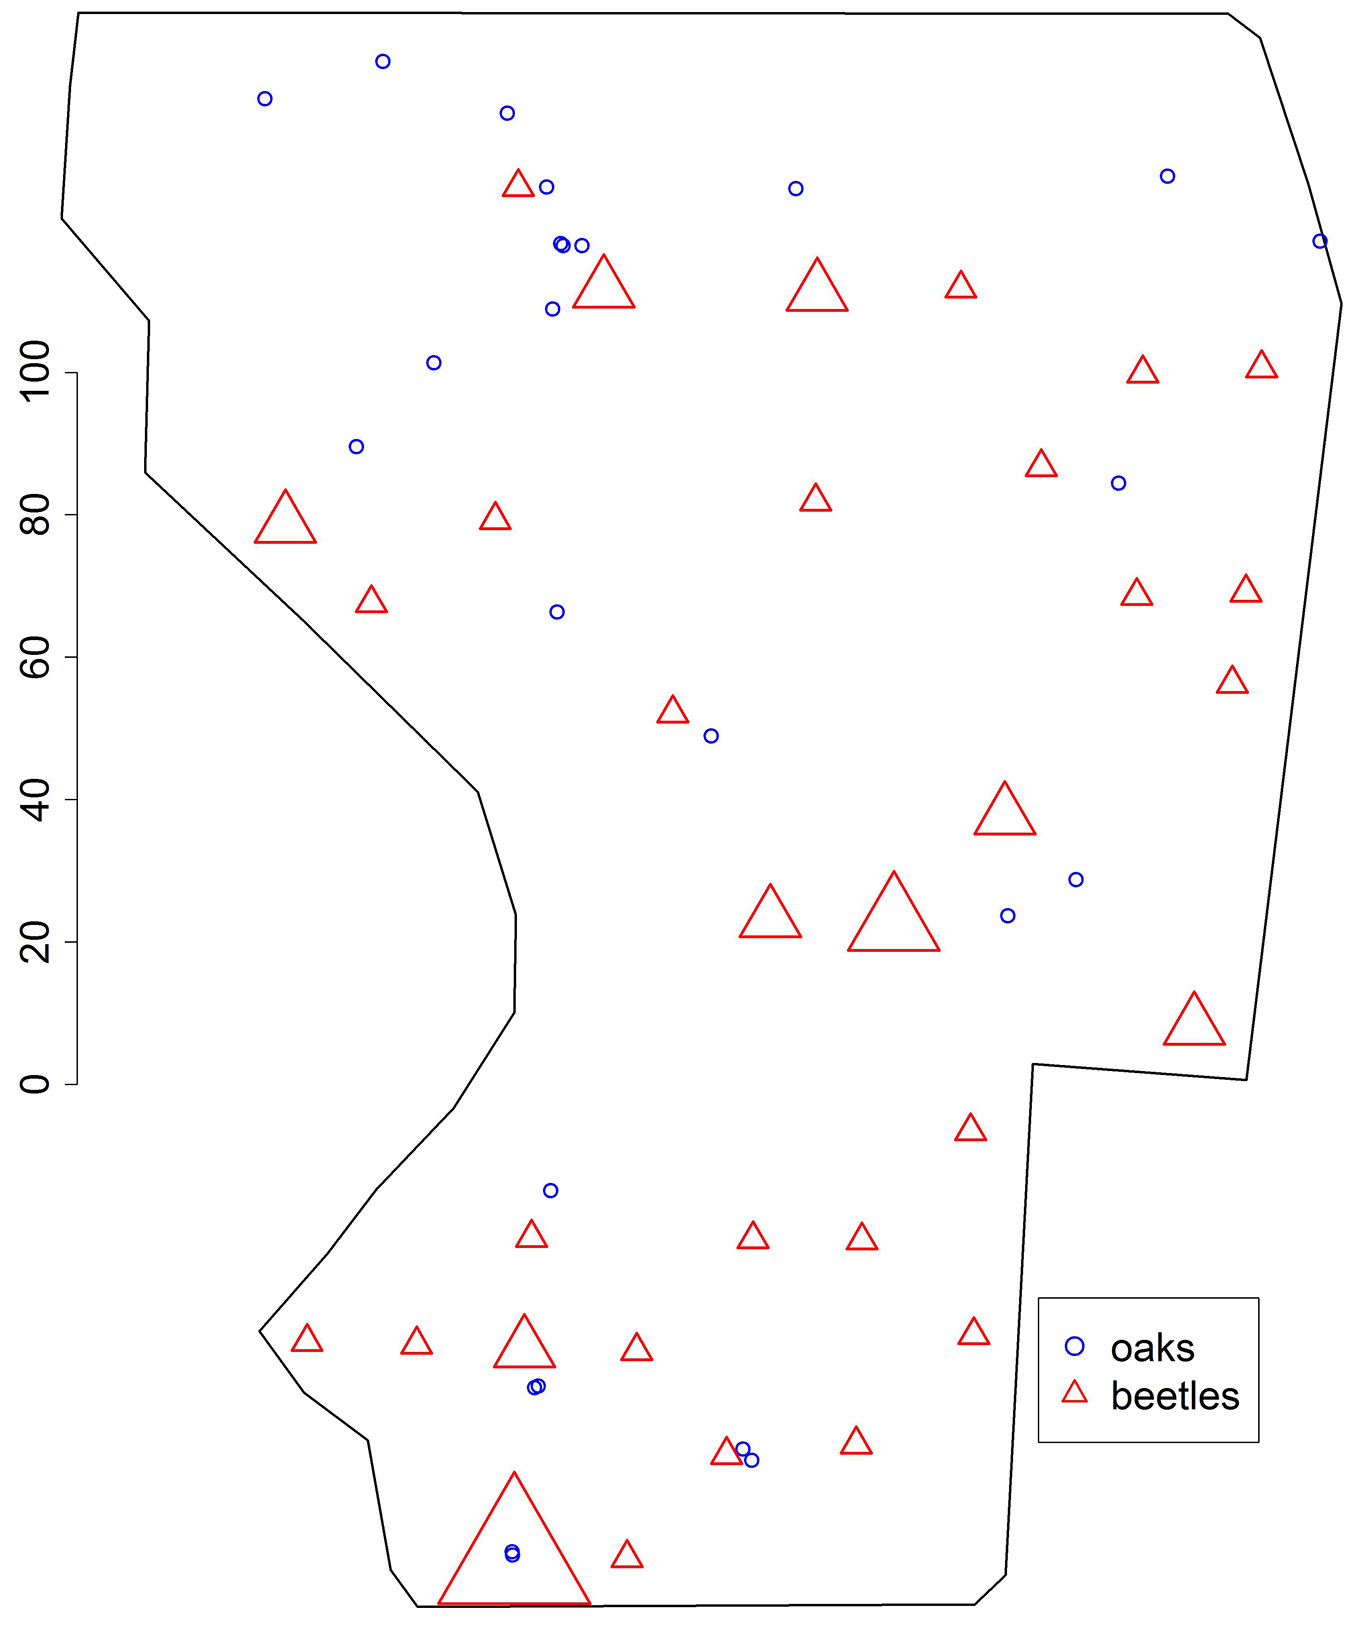
\includegraphics[scale=0.05]{iForest_ifor1952-009-image001}\caption{Wagner et al., iForest 2016}\end{figure}
\end{column}
\begin{column}{0.6\textwidth}
\begin{itemize}
\item Typically $D \in R^2$.
\item Random realisation of point pattern by $\bm{S}=\{s_1, \ldots, s_n\}$.
\item $\bm{S}$ is random and characterised by
\begin{itemize}
\item $N(D)$: number of points in $D$
\item Multivariate density $D^n$ for $f(s_1,\ldots,s_n)$ (location density).
\end{itemize}
\item Spatial point process. 
\end{itemize}
\end{column}
\end{columns}
\end{frame}
%%%%%%%%%%%%%%%%%%%%%%%%%%%%%%%%%%%%%%%%%%%%%%%%%%%%%%%%%%%%%%%%%%%%%
\begin{frame}    \frametitle{Types of spatial data [cont'd]}
\begin{itemize}
\vfill  \item \textbf{Point-referenced data}: the exact location of the occurrences is known
        \begin{itemize}
\vfill        \item can be collected through specialized survey / monitoring network...
\vfill        \item if locations are \emph{fixed} (monitoring stations, postcodes in an area)
         and the variable of interest is measured at each location (e.g. presence/absence of cases, pollution concentrations)\\
         $\Rightarrow$ \alert{geostatistical framework.}
        \end{itemize}
        
\vfill  \item \textbf{Area data or count data}: locations are areal units with well defined geographical boundaries, usually administrative units
        \begin{itemize}
\vfill        \item outcome is number of cases aggregated over the area\\
$\Rightarrow$ \alert{small area framework.}
        \end{itemize}

\end{itemize}
\end{frame}
%%%%%%%%%%%%%%%%%%%%%%%%%%%%%%%%%%%%%%%%%%%%%%%%%%%%%%%%%%%%%%%%%%%%%%%%%%%%%%%%%%%%%%%%
\section{Small area framework}
\begin{frame}
\begin{center}
\vfill\fontsize{20}{20}\selectfont{Small area framework}\end{center}
\end{frame}
%%%%%%%%%%%%%%%%%%%%%%%%%%%%%%%%%%%%%%%%%%%%%%%%%%%%%%%%%
\begin{frame}\frametitle{General inferential issues}


Spatial (and temporal) pattern suggests that observations close to each other have more similar
	values than those far from each other.
	
%\vfill\item When are we interested in the spatial and temporal components?


	\begin{itemize}
%\vfill	\item Are we explicitly interested in the spatial pattern of disease risk?\\
\pause\vfill		\item Do we want to smooth the data?\\ $\rightarrow$ Disease mapping, cluster detection.\\
	$\rightarrow$ {\bf In this talk}: \alert{Space-time-age disease mapping}\\
\pause\vfill		\item Do we want to evaluate temporal trends for each area?\\
	$\rightarrow$ Discover unusual patterns.\\ 
	$\rightarrow$ {\bf In this talk}: \alert{Disease surveillance}\\
	
\pause\vfill	\item Is the spatial clustering and/or temporal trend a nuisance quantity that we wish to take into account but are not explicitly interested in?\\ $\rightarrow$ Spatial regression\\
	$\rightarrow$ {\bf In this talk}: \alert{Leukaemia and benzene in Greater London}\\
\pause	\vfill\item Is the regression coefficient spatially varying?\\
		$\rightarrow$ {\bf In this talk}: \alert{Case-crossover design for spatio-temporal epidemiological investigations}\\
\end{itemize}
\end{frame}
%%%%%%%%%%%%%%%%%%%%%%%%%%%%%%%%%%%%%%%%%%%%%%%%%%%%%%%%%
\begin{frame}
    \frametitle{General framework - I}
\begin{itemize}
\item \textbf{Data} for a region of interest, a geographical level and a specific period:
		%\uncover<2-> England, ward level, 2009-2012
        \begin{itemize}
            \vfill\item $O_i$: Observed number of cases in area $i$\\
				Lung cancer deaths in males aged 45+\\
				Number of reported crimes \\
				Number of people reporting confidence in the police\\
            \pause\vfill\item $n_i$ (or $E_i$): Population at risk in area $i$ (or expected number of cases)\\
            Male population aged 45+\\
            Resident Population or nb of dwellings\\
            Number of people surveyed in each borough neighborhood\\                
        \end{itemize}
\pause\vfill\item \textbf{Parameter of interest} Relative risk $\lambda$ in each area compared with the chosen reference area.
\end{itemize}
\end{frame}
%%%%%%%%%%%%%%%%%%%%%%%%%%%%%%%%%%%%%%%%%%%%%%%%%%%%%%%

\begin{frame}\frametitle{General framework - II}
\begin{itemize}
\item Standard statistical model for rare outcomes/small areas
\begin{equation*} O_i \sim \hbox{Poisson}(\lambda_i E_i) \end{equation*}
 
 \begin{itemize}
 \item SMR$_i= \frac{O_i}{E_i}$ is the MLE for $\lambda_i$;
\item $\hbox{SMR}_i$ very imprecise for rare events and/or areas with small populations, $\lambda_i$ estimated variance is $\frac{O_i}{E_i^2}$;\\
$\Rightarrow$ Highlights extreme risk estimates based on small numbers.
    \end{itemize}
\vspace{0.2cm}
\pause\item SMR in each area is estimated independently\\
$\rightarrow$ makes no use of risk estimates in other areas of the map, even though these are likely to be similar.
\vspace{0.2cm}
\item Ignores possible spatial correlation between disease risk in nearby areas 
\end{itemize}

\pause\centering\color{red}{Bayesian `smoothing' estimators in a hierarchical formulation.}

\end{frame}


\begin{frame}
    \frametitle{Hierarchical modelling for small area data}
\begin{block}{Poisson-logNormal model}
\vspace{-0.5cm}
\begin{eqnarray*}
O_i & \sim & \hbox{Poisson}(\lambda_i E_i) \\
\log \lambda_i & = & \alpha + v_i\\
v_i & \sim  & \hbox{Normal}(0, \sigma_v^2)
\end{eqnarray*}

%{\small
%Priors (vague, non informative):
%\vspace{-0.2cm}
%\begin{itemize}
%  \item between-area sd: $\sigma_v \sim \text{Truncated Normal}(0,100)_{[0,Inf)}$
%  \vspace{-0.2cm}
%  \item mean log relative risk: $\alpha \sim flat()$
%\end{itemize}}
\end{block}
where
\begin{itemize}
  \item $O_i$, $E_i$: observed and expected nb of cases in area $i$
  \item $\lambda_i=\exp (\alpha +  v_i)$: RR in area $i$ compared with expected risk (for instance based on age and sex of population)
  \item Parameters $v_i$: {\bf area-specific random effects}
  \item residual RR = $\exp (v_i)$.
% \lambda as relative risk (number of cases in the area compared to the expected - accounting for all the risk factors in the area compared with the normal age and sex in the population
\end{itemize}
\end{frame}
%%%%%%%%%%%%%%%%%%%%%%%%%%%%%%%%%%%%%%%%%%%%%%%%%%%%%%%%
\begin{frame}
    \frametitle{Lung cancer incidence in males, 1985-2009, England and Wales}
    \begin{center}
    RR estimates using 2 methods
        \scalebox{0.6}{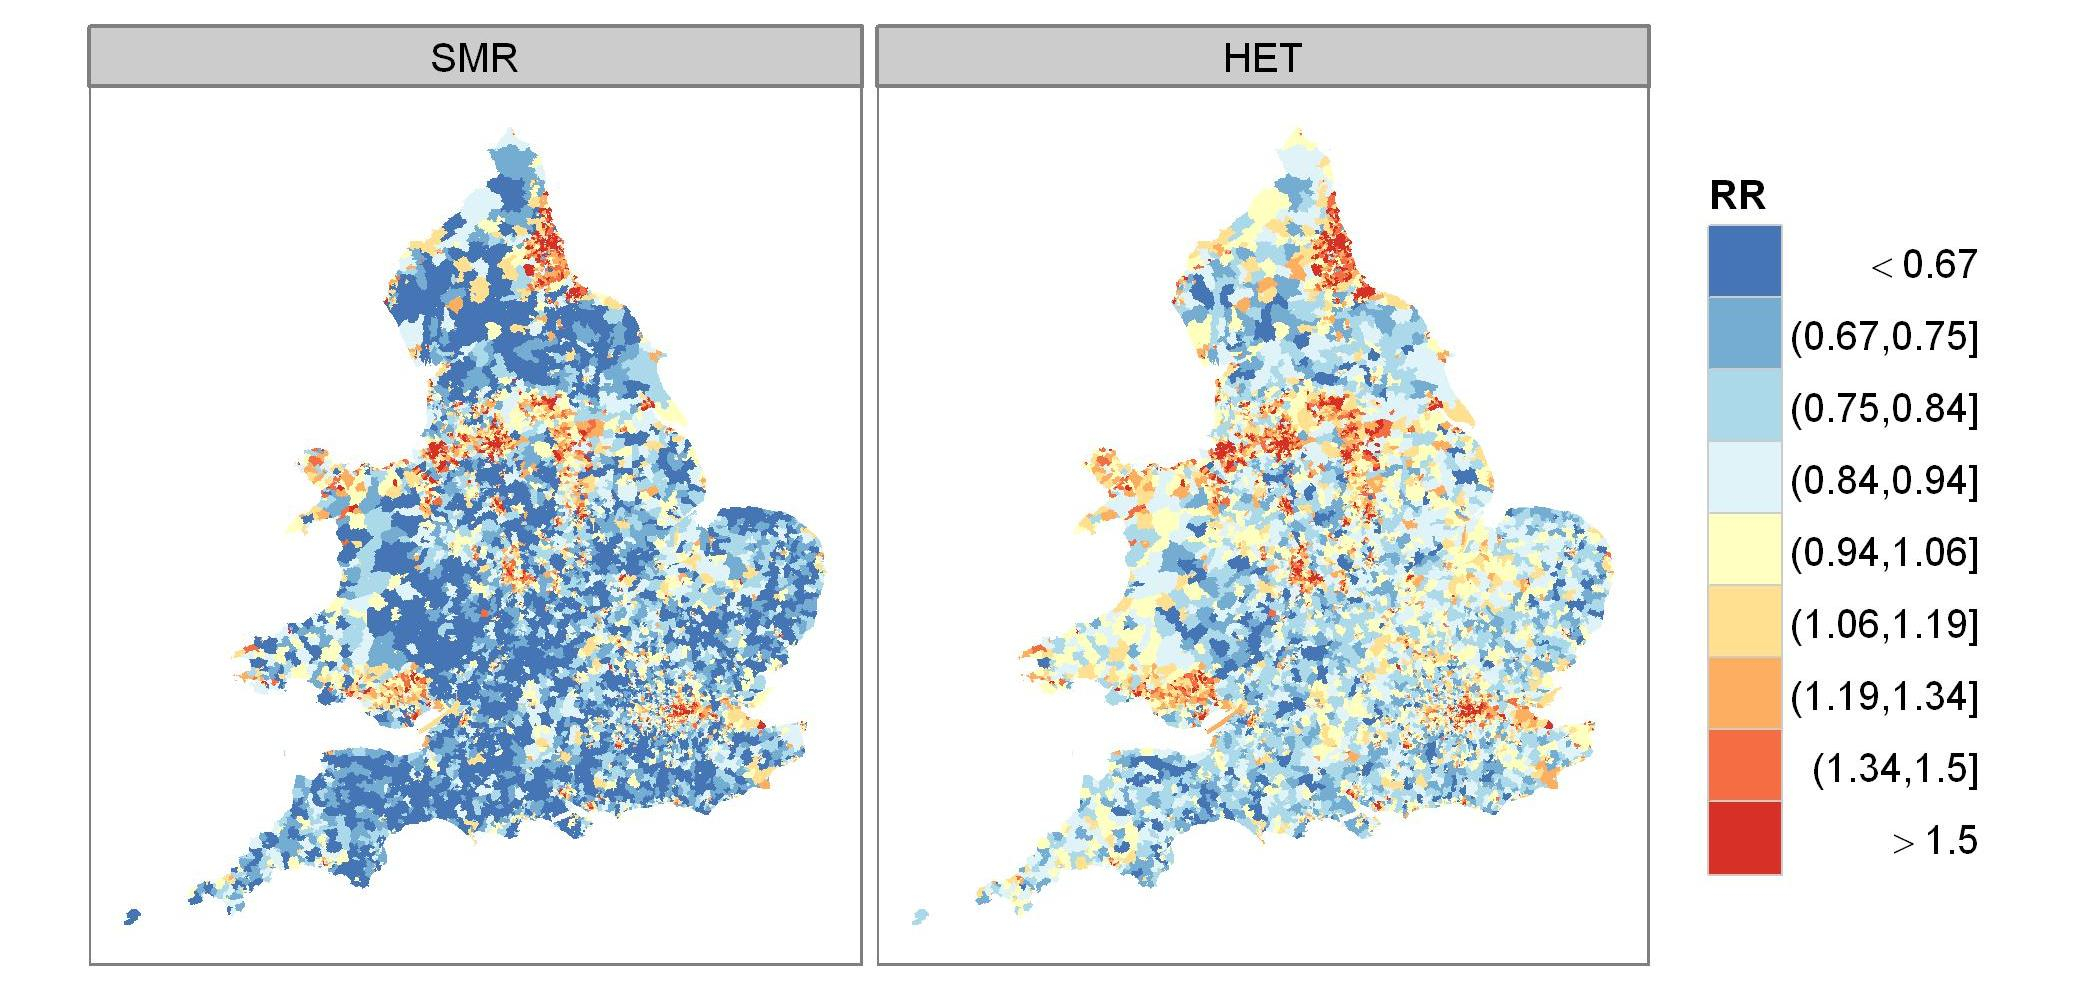
\includegraphics{Lungmales_SMRHETmap.jpg}}\\
        SMRs and smoothed RRs
    \end{center}
\end{frame}

%%%%%%%%%%%%%%%%%%%%%%%%%%%%%%%%%%%%%%%%%%%%%%%%%%%%%%%%
\begin{frame}\frametitle{Local spatial dependency}

To account for local dependency it is possible to add a spatial structure in the model:
\begin{block}{Convolution model}
\vspace{-0.5cm}
\begin{eqnarray*}
O_i & \sim & \hbox{Poisson}(\lambda_i E_i) \\
\log \lambda_i & = & \alpha + v_i + u_i\\
v_i & \sim  & \hbox{Normal}(0, \sigma_v^2)\\
u_i \mid u_{-i} & \sim & \hbox{Normal}\left(\frac{\sum_{k=1}^n w_{ik} u_k}{\sum_{k=1}^n w_{ik}}, \frac{\sigma^2_u}{\sum_{k=1}^n w_{ik}}\right)\end{eqnarray*}
\end{block}
\begin{itemize}
  \item $u_i$ follows a conditional autoregressive specification (CAR); it assumes that only neighbouring areas contribute to the distribution of area $i$ ($w_{ik}=1$).
  \item The combination of $v_i$ and $u_i$ guarantees local and global smoothing (BYM model).
\end{itemize}

\fontsize{7}{7}\selectfont{Besag, J., et al. (1991). ``Bayesian image restoration, with two applications in spatial statistics''. \textbf{Annals of the Institute of Statistical Mathematics}, 43, 1-59.}
\end{frame}
%%%%%%%%%%%%%%%%%%%%%%%%%%%%%%%%%%%%%%%%%%%%%%%%%%%%%%%%

\begin{frame}\frametitle{Residual RR of lung cancer incidence in males, 1985-2009, England and Wales II}

\begin{center}\begin{tikzpicture}[remember picture, overlay]
  \node (img1) at (-2.8,-3.2) {{\visible<1->{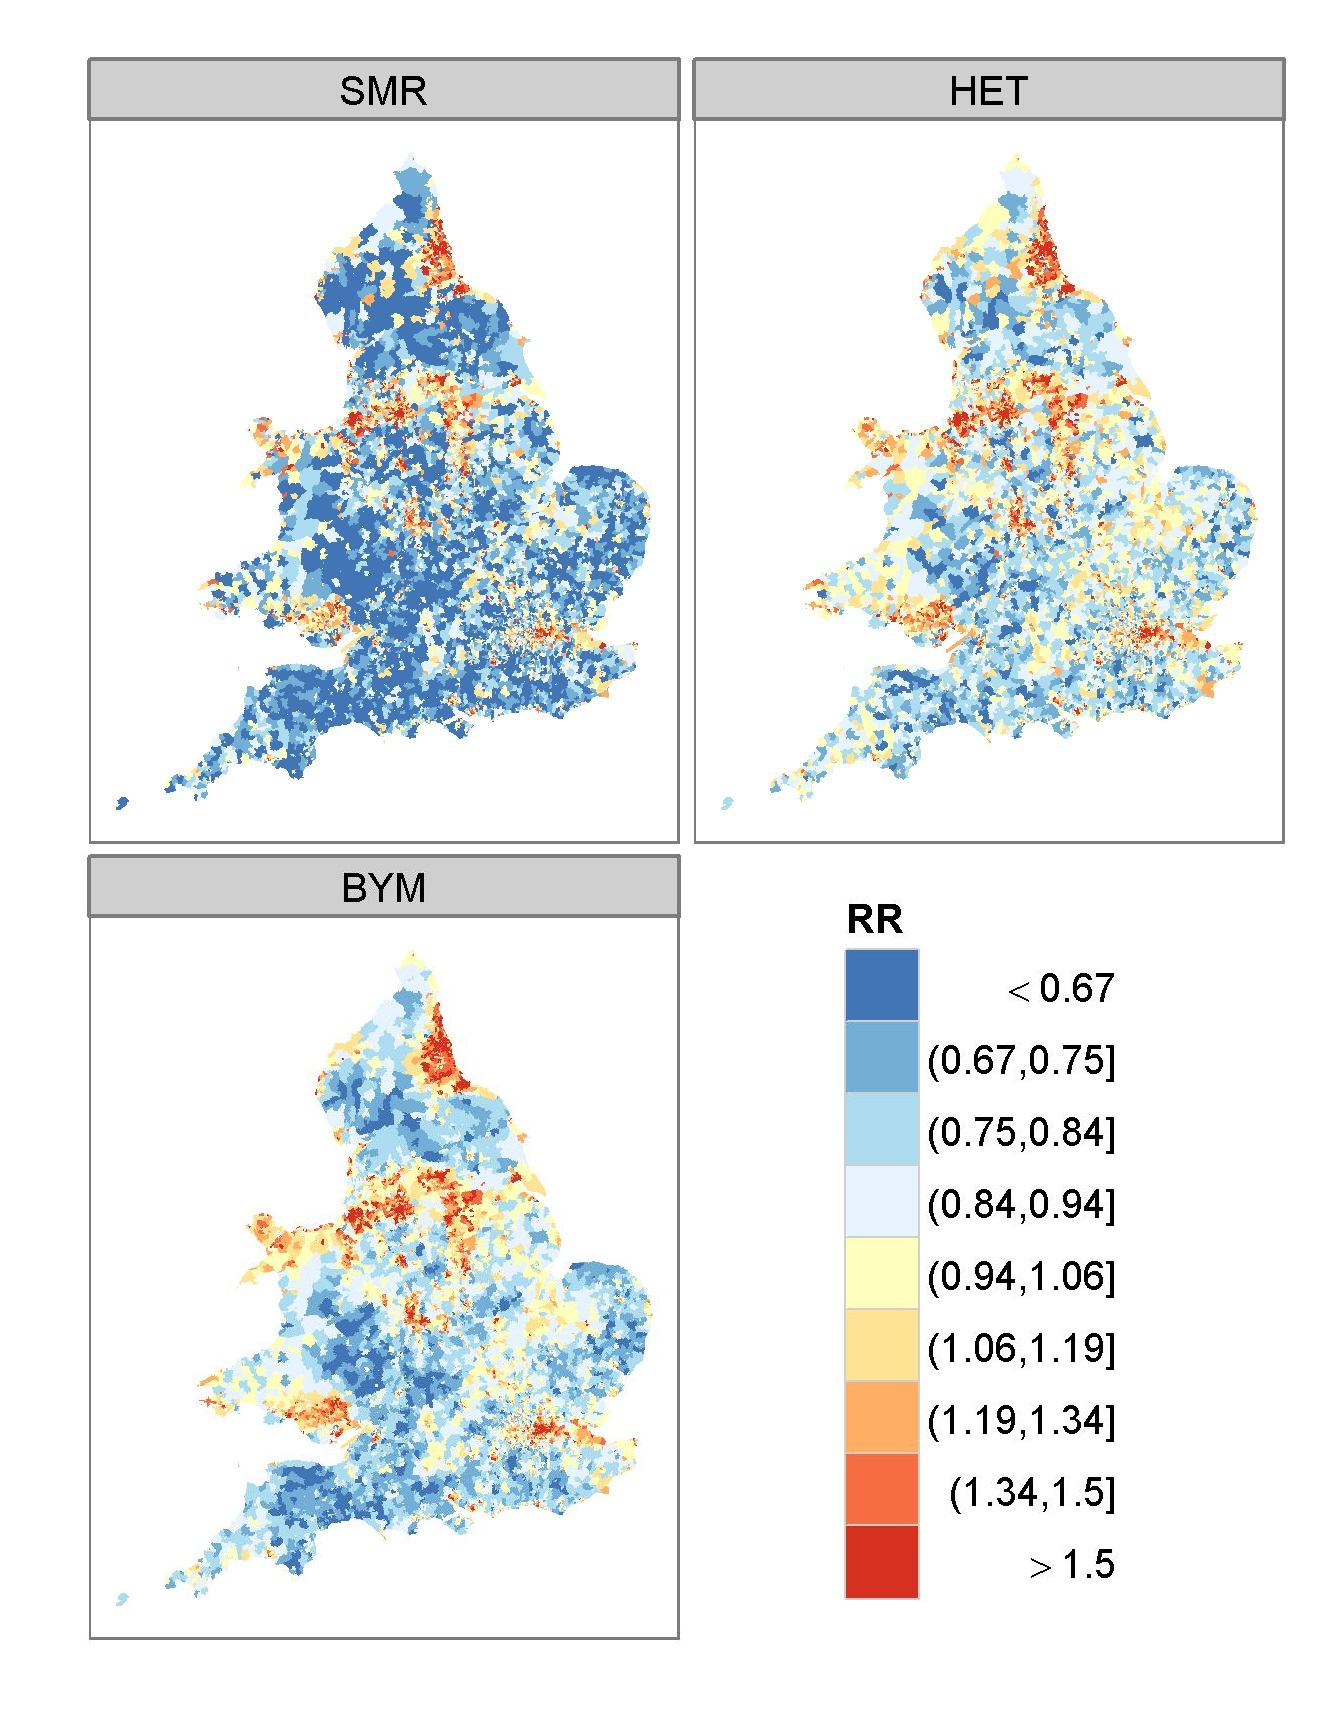
\includegraphics[scale=.5]{Lungmales_3maps.jpg}}}};
  \node[right=1cm of img1,text width=5cm](text){\textbf{SMR}: non smoothed RR\\ \vspace{10pt}\textbf{HET}: non spatially smoothed residual RR $\exp(v)$\\ \vspace{10pt}\textbf{BYM}: spatially and non spatially smoothed residual RR $\exp(v+u)$};
\end{tikzpicture}
\end{center}
\end{frame}
%\begin{tabular}{cc}
%\vspace{-250pt}\begin{minipage}[t]{3.5cm}
%\begin{itemize}
%\item[SMR] non smoothed RR
%\item[HET] non spatially smoothed residual RR $\exp(v)$
%%\item[CAR] spatially smoothed residual RR $\exp(u)$
%\item[BYM] spatially and non spatially smoothed residual RR $\exp(v+u)$
%\end{itemize}
%\end{minipage}
%&
%
%\noindent \begin{minipage}[t]{7cm}
%\begin{center}
%{\scalebox{0.5}{
%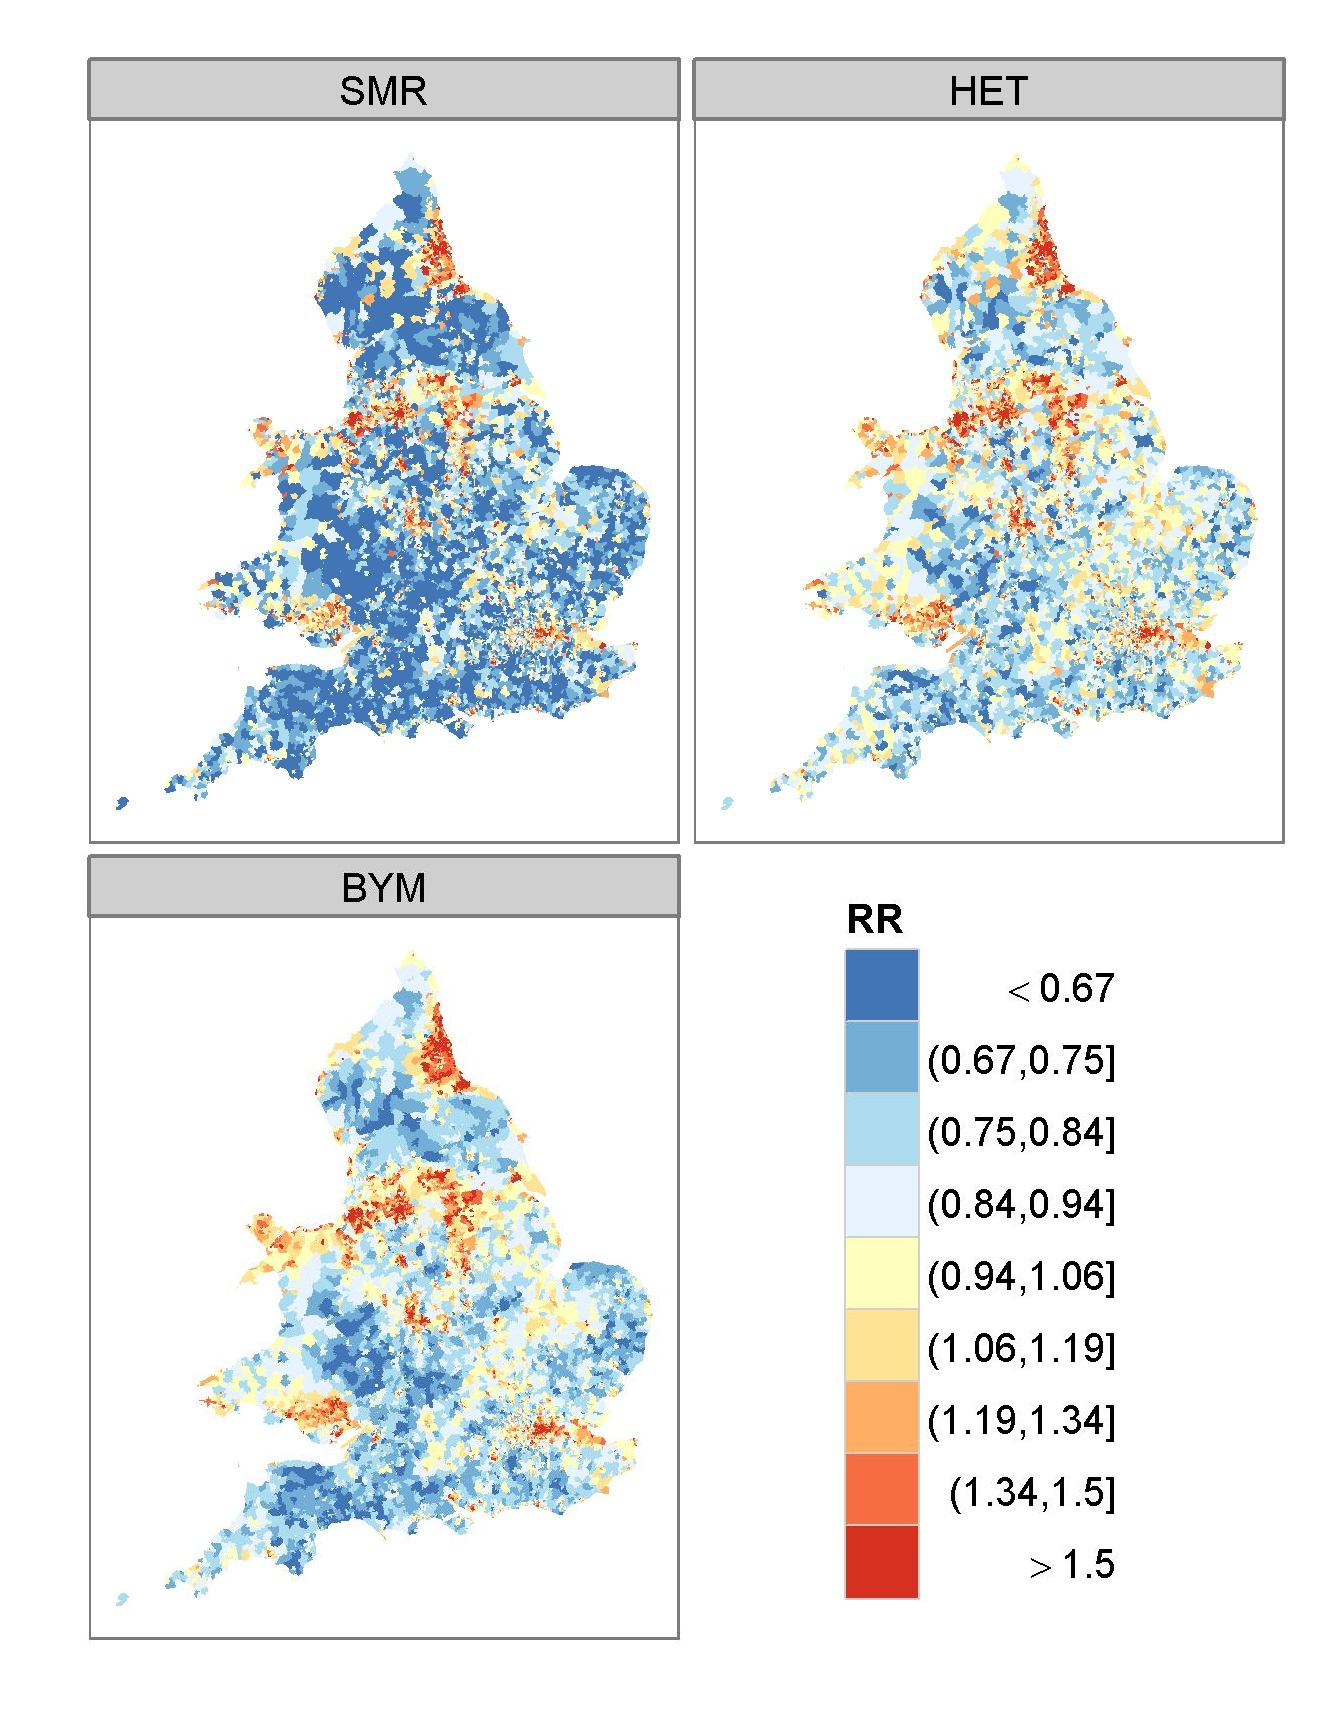
\includegraphics{Lungmales_3maps.jpg}
%}}
%\end{center}
%\end{minipage}\end{tabular}
%}
%%%%%%%%%%%%%%%%%%%%%%%%%%%%%%%%%%%%%%%%%%%%%%%%%%%%%%%%%%%%%%%%%%%%%%%%%%%%%%%%%%%%%%%%%%
\frame{\frametitle{Extending space to space-time}
\begin{itemize}
\vfill \item The hierarchical structure can be extended to incorporate time into a space-time model.
\vfill \item The stability (or not) of the
spatial pattern can aid interpretation.
\vfill \item The specific
space-time components of the model can potentially pinpoint
unusual / emerging risk factors.
\end{itemize}

\pause\begin{block}{Spatio-temporal hierarchical model}
\vspace{-0.5cm}
\begin{eqnarray*}
O_{it} & \sim & \hbox{Poisson}(\lambda_{it} E_{it}) \\
\log \lambda_{it} & = & \alpha + v_i + u_i + \phi_t +  \gamma_t +\psi_{it}\\
\end{eqnarray*}

{\small
Temporal trend and space-time interaction:
\vspace{-0.2cm}
\begin{itemize}
  \item Temporal trends: $\phi_t \sim \text{Normal}(\phi_{t-1}, \sigma^2_{\phi})$; \\
  \hspace{70pt} $\gamma_{t} \sim \text{Normal}(0,\sigma^2_{\gamma})$
  \vspace{-0.2cm}
  \item Space-time interaction: $\psi_{it} \sim \text{Normal}(0,\sigma^2_{\psi})$
\end{itemize}}
\end{block}
\fontsize{7}{7}\selectfont{Knorr-Held, L., ``Bayesian modelling of inseparable space-time variation in disease risk'', \textbf{Statistics in Medicine}, 2000, 19(17-18): 2555:2567.}
}
%
%\frame{\frametitle{Schematic representation I}
%\begin{center}
%\scalebox{0.45}
%{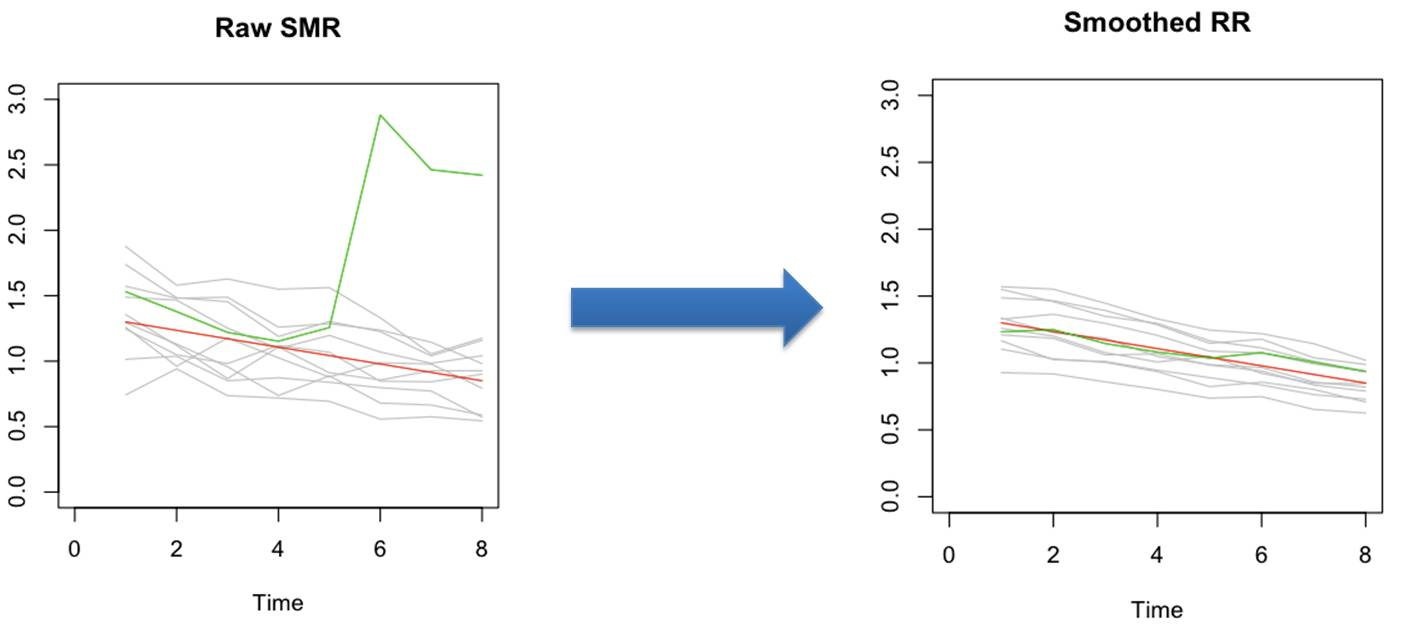
\includegraphics{representation_ST1.jpg} }
%\end{center}
%}
%
%\frame{\frametitle{Schematic representation II}
%\begin{center}
%\scalebox{0.45}
%{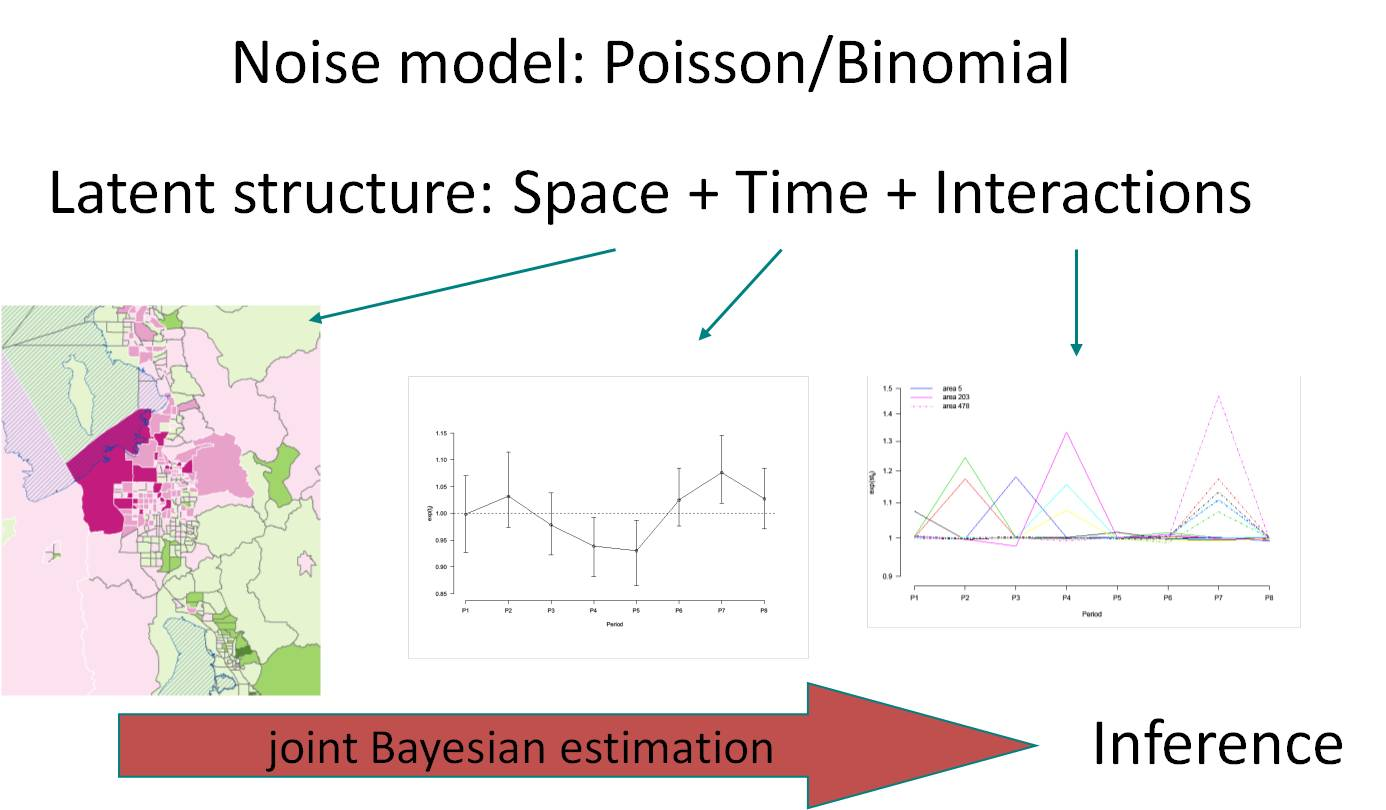
\includegraphics{representation_ST.jpg} }
%\end{center}
%}
%%%%%%%%%%%%%%%%%%%%%%%%%%%%%%%%%%%%%%%%%%%%%%%%%%%%%%%%
\subsection{Examples}
\begin{frame}\frametitle{Example: schistosomiasis japonica in East China}
\begin{itemize}
\item Spatio-temporal model of schistosomiasis japonica;
\item Interested in evaluating changes in time (discover policy effects). 
%WHICH POLICY
\end{itemize}
\begin{center}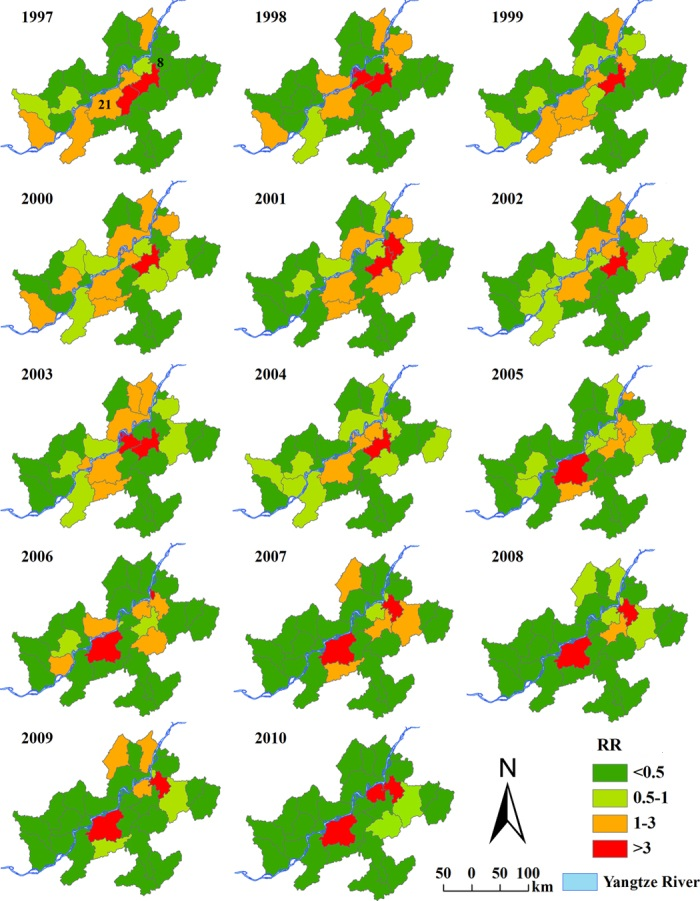
\includegraphics[scale=0.75]{srep24173-f3}\end{center}

\fontsize{7}{7}\selectfont{Hu, Y et al., ``Monitoring schistosomiasis risk in East China over space and time using a Bayesian hierarchical modeling approach'', \textbf{Scientific Reports}, 2012, 6: 24173.}
\end{frame}
%%%%%%%%%%%%%%%%%%%%%%%%%%%%%%%%%%%%%%%%%%%%%%%%%%%%%%%%
\begin{frame}\frametitle{Adding another dimension}
\begin{itemize}
\vfill\item Detect spatio-temporal patterns according to the different age groups $j=1,\ldots,J$
\vfill\begin{eqnarray*}
\log \lambda_{itj} & = & \alpha + u_i + \phi_t + \xi_j + \psi^1_{it} + \psi^2_{jt} + \psi^3_{ij} + \zeta_{itj}\\
\end{eqnarray*}
\vfill\item Autoregressive structure on $u_i$;
\vfill\item Random walk on $\phi_t$ and $\xi_j$;
\vfill\item Structured interactions:\\ 
$\rightarrow$ temporal trends are different for far apart regions but tend to be similar for adjacent regions;\\
$\rightarrow$ temporal trends and spatial patterns are similar for subsequent age classes.

%\begin{eqnarray*}
%\boldsymbol{\psi}^1 \sim MVN(\bm{0}, \sigma^2_{\omega\phi}D_{\omega\phi})\\
%\end{eqnarray*}
%\item $D_{\omega\phi}$ is the Kronecker product of marginal covariance matrices.
\end{itemize}

\fontsize{7}{7}\selectfont{
Goicoa T et al., ``Age-space-time CAR models in Bayesian disease mapping'', \textbf{Statistics in Medicine}, 2016, 35(14):2391-2405.}

\end{frame}
%%%%%%%%%%%%%%%%%%%%%%%%%%%%%%%%%%%%%%%%%%%%%%%%%%%%%%%%
\begin{frame}\frametitle{Example: Age-space-time CAR models in disease mapping}
\begin{itemize}
\item Prostate cancer mortality in Spain. 
\item Data are available in 50 provinces and 9 age groups during 25 years between 1986 and 2010.
\end{itemize}
%CHECK SCALE
\begin{tikzpicture}[remember picture, overlay]
  \node (img1) at (3,-2.7) {{\visible<1->{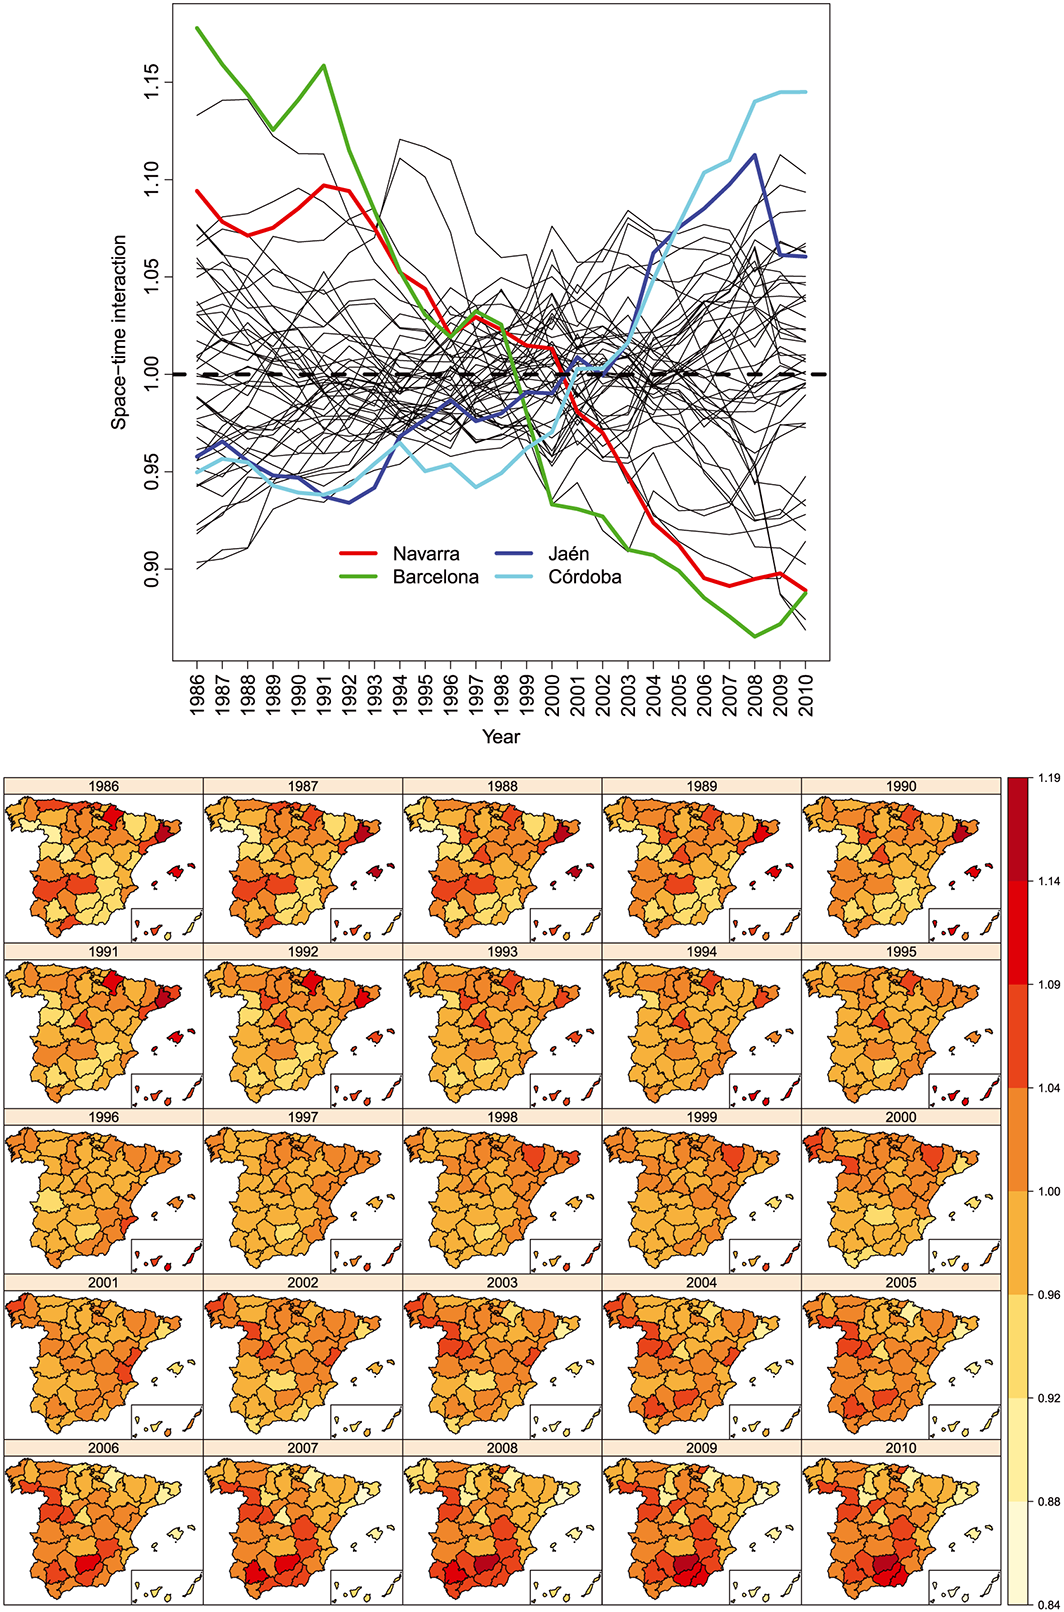
\includegraphics[scale=0.14]{sim6873-fig-0005}}}};
  \pause
  \node (img2) at (5,-3) {{\visible<2->{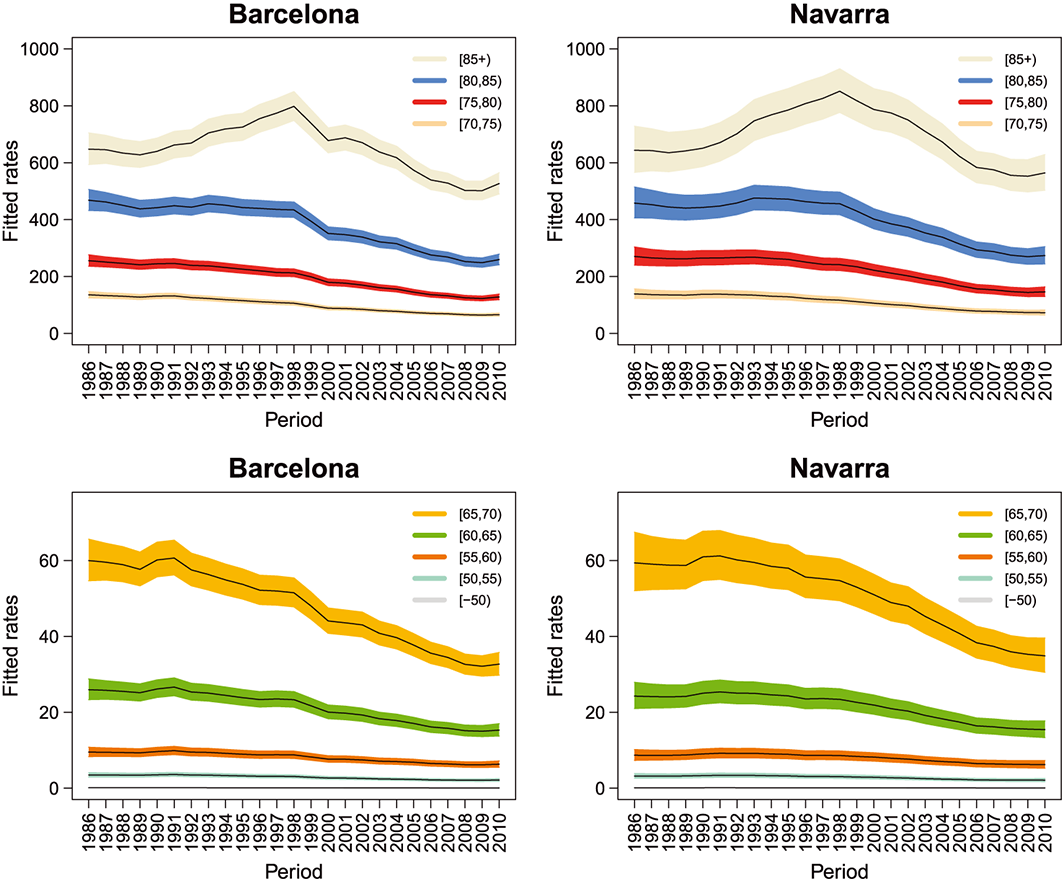
\includegraphics[scale=0.2]{sim6873-fig-0006}}}};
  \pause
 \node (img3) at (6,-2){{\visible<3-3>{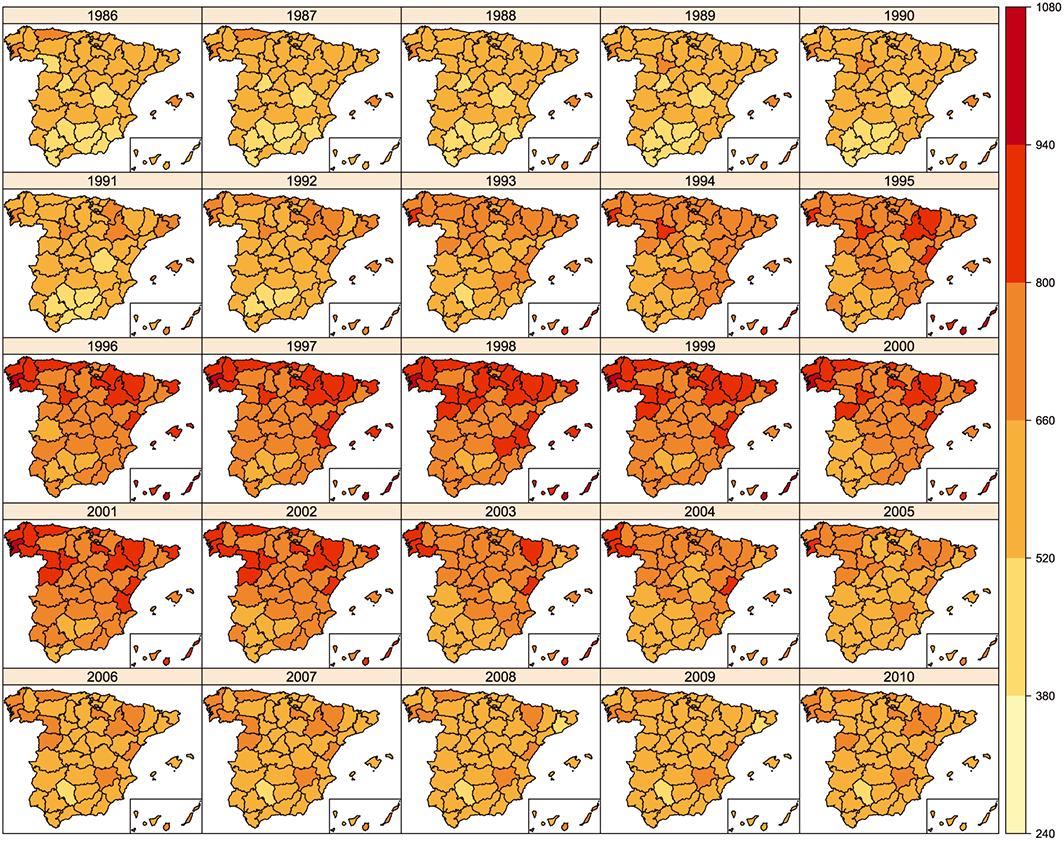
\includegraphics[scale=0.2]{sim6873-fig-0007}}}};
\end{tikzpicture}

\end{frame}
%%%%%%%%%%%%%%%%%%%%%%%%%%%%%%%%%%%%%%%%%%%%%%%%%%%%%%%%%%%%%%%%
\begin{frame}{Spatio-temporal mixture model}
\begin{itemize}
\item Extend the spatio-temporal hierarchical framework to a mixture model with two components
    \begin{itemize}
    \vfill\item accounts for spatial  and temporal correlation;
\vfill\item able to detect areas with trend different from the national one (unusual).
   \end{itemize}
\end{itemize}

 \begin{center}$O_{it} \sim \mbox{Poisson}(\lambda_{it}\; E_{it})$ \end{center}
  \vskip0pt plus.5fill
\small{areas  $i=1, \dots, I$; time points $t=1, \dots, T$}.
\medskip
\begin{align*}
\begin{split}
 \mbox{log} (\lambda_{it}) = p_{it} \;  \mbox{log}\big(\,\lambda_{it}^{\mbox{C}}\,\big)  + (1-p_{it}) \; \mbox{log}\big(\, \lambda_{it}^{\mbox{AS}}\, \big)  
\end{split}
\end{align*}

\begin{center}\begin{tikzpicture}
\draw[blue, thick, ->] (0.8,0) -- (1.5, -1);
\draw[blue, thick, ->] (-0.8,0) -- (-1.5,-1);
\end{tikzpicture}\end{center}


\begin{columns}
\begin{column}[T]{0.37\textwidth}
\textcolor{blue}{Common Trend}
\begin{itemize}
\item[$\bullet$] overall intercept
\item[$\bullet$]  spatial component
\item[$\bullet$]  temporal component
\end{itemize}
%\[  \mbox{log}\big(\,\mu_{it}^{\mbox{C}}\,\big) =\quad  \alpha_0 + h_i + \gamma_t\]
%\[  \alpha_0 \sim  \quad \mbox{U}(-\infty, +\infty)\]
%\[ h_i \sim \mbox{N}(v_i,\sigma^2_h) \; \; and \;  \; v_i \sim \mbox{CAR}(\mbox{W}, \sigma^2_v)\]
%\[ \gamma_{t} \sim  \quad \mbox{CAR}(\mbox{Q}, \sigma^2_\gamma) \]
\end{column}
\begin{column}[T]{0.4\textwidth}
\textcolor{blue}{Area-Specific Trend}
\begin{itemize}
\item[$\bullet$]  area-specific intercept
\item[$\bullet$] area-specific temporal component
\end{itemize}
%\[ \mbox{log}\big(\, \mu_{it}^{\mbox{AS}}\, \big)=  \quad u_i + k_{it}\]
%\[ u_i \sim \quad \mbox{N}(0,1000) \]
%\[k_{i, t} \sim  \quad \mbox{CAR}(\mbox{Q}, \sigma^2_{i,k}) \]
%\[\mbox{log}(\sigma^2_{i,k}) \sim  \quad \mbox{N}(\alpha, \beta^2) \]
\end{column}
\end{columns}

\vspace{5pt}\fontsize{7}{7}\selectfont{
Li G., et al., ``BaySTDetect: detecting unusual temporal patterns in small area data via Bayesian model choice'', \textbf{Biostatistics}, 2012, 13(4): 695-710.
}
\end{frame}

%%%%%%%%%%%%%%%%%%%%%%%%%
%\begin{frame}
%\frametitle{Modelling the probability for the two components}
%\begin{itemize}
%\item Each area is characterised by a (vector of) probability $\bm p_{i}=\left( p_{i1}, \ldots, p_{iT} \right)$ of being assigned to the common trend component - used to assign the area as common/uncommon.
%\item $p_{it}$ can be modelled as a combination of several effect:
%\begin{itemize}
%\item local and global dependency in space (clusters or isolated areas);\\
%\begin{center}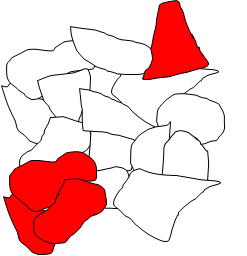
\includegraphics[scale=0.26]{Cluster.png}\end{center}
%\item local and global dependency in time (similar trend or isolated time points).\\
%\begin{center}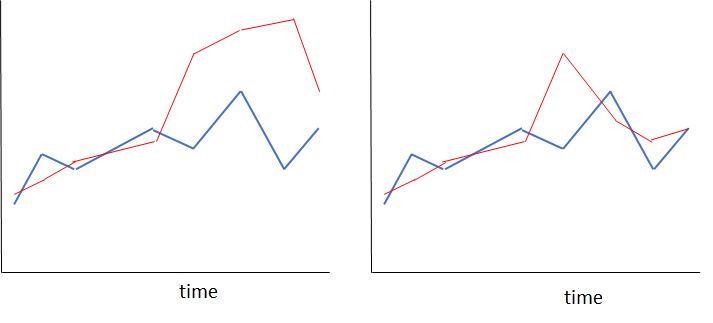
\includegraphics[scale=0.26]{TimeCluster.png}\end{center}
%\end{itemize}
%\end{itemize}
%\end{frame}
%%%%%%%%%%%%%%%%%%%%%%%%%%
%\begin{frame}
%\frametitle{Implementation}
%\begin{itemize}
%\vfill\item Bayesian formulation - priors on all the parameters
%\vfill\item Inference is performed through Markov Chain Monte Carlo simulative approach
%\vfill\item The model is currently implemented in OpenBUGS via R\end{itemize}
%\end{frame}
%%%%%%%%%%%%%%%%%%%%%%%%%%%%%%%%%%%%%%%%%%%%%%%%%%%%%%%%
\begin{frame}{Example: Unusual trend detection for COPD}

 \begin{block}{}
{\bf COPD hospital admissions}.\\ Spatial resolution: 211 Clinical Commissioning Groups (CCGs)\\
Temporal resolution: monthly data, April 2010 - March 2011.\\
\end{block}
 % \vskip0pt plus.5fill
\centering
\begin{figure}\caption{HES SMRs}
\animategraphics[autoplay,loop, width=4.8cm]{1}{SMR}{1}{12}
\end{figure}
\end{frame}

%%%%%%%%%%%%%%%%%%%%%%%%%
\begin{frame}{Results: Spatial pattern}

%\begin{figure}[h]
\begin{tabular}{m{5cm}m{5cm}}
\footnotesize{Spatial Posterior Mean} & \hspace{30pt}\footnotesize{Unusual Areas}\\
\end{tabular}
\begin{columns}
\begin{column}{0.5\textwidth}               
%\begin{subfigure}[b]{0.45\textwidth} 
%               \caption{\footnotesize{Spatial Posterior Mean}}
%\footnotesize{Spatial Posterior Mean}\\
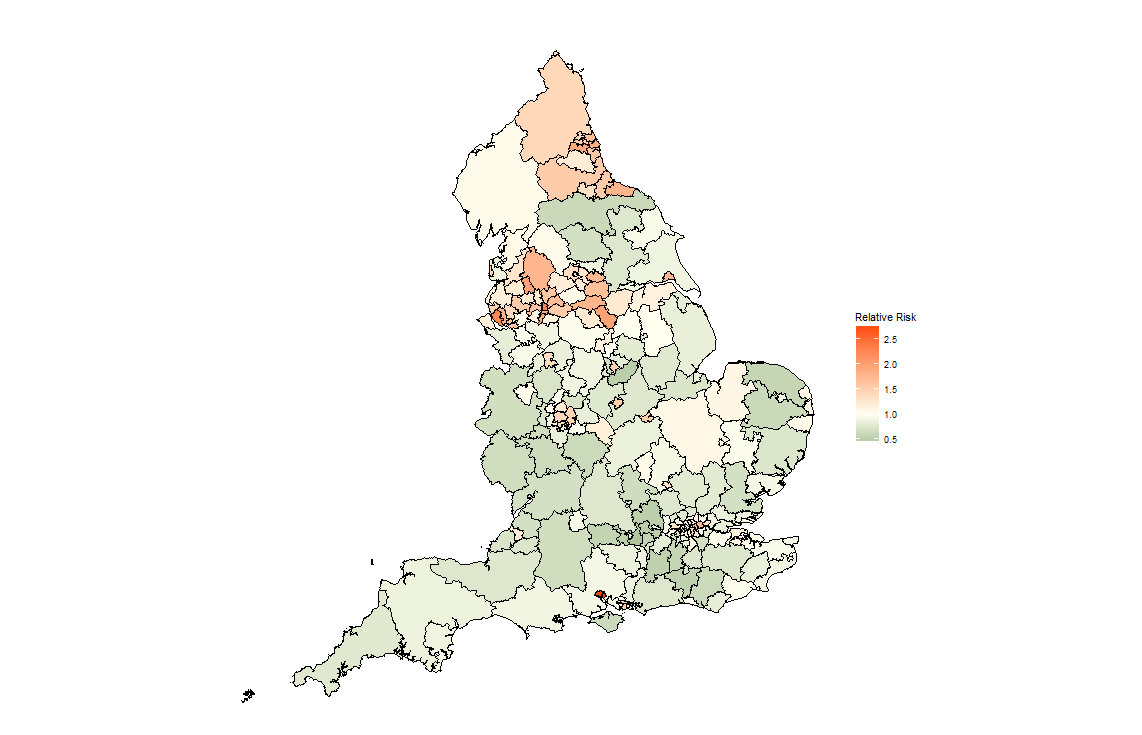
\includegraphics[width=\textwidth]{RRmap}
\end{column}

                 %\end{subfigure}
%            \begin{subfigure}[t]{0.55\textwidth}
%            \caption{\footnotesize{Unusual areas}}
\begin{column}{0.5\textwidth}               
%\footnotesize{Unusual Areas}\\
                 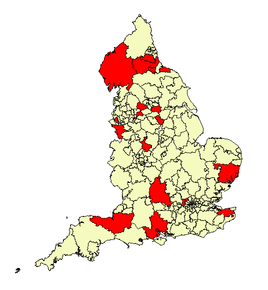
\includegraphics[width=0.6\textwidth]{outbreaks_map}
\end{column}
\end{columns}
%        \end{subfigure}
%\end{figure}
\begin{itemize}
\vfill\item Higher risk in the north of England across the time period.
\vfill\item Unusual areas: mostly isolated but some clustered in the North of England.
\end{itemize}

\end{frame}

\begin{frame}\frametitle{Results: Unusual trends}
\begin{center}
\begin{tikzpicture}[overlay]
  \node (img1) at (0,-2.7) {{\visible<1->{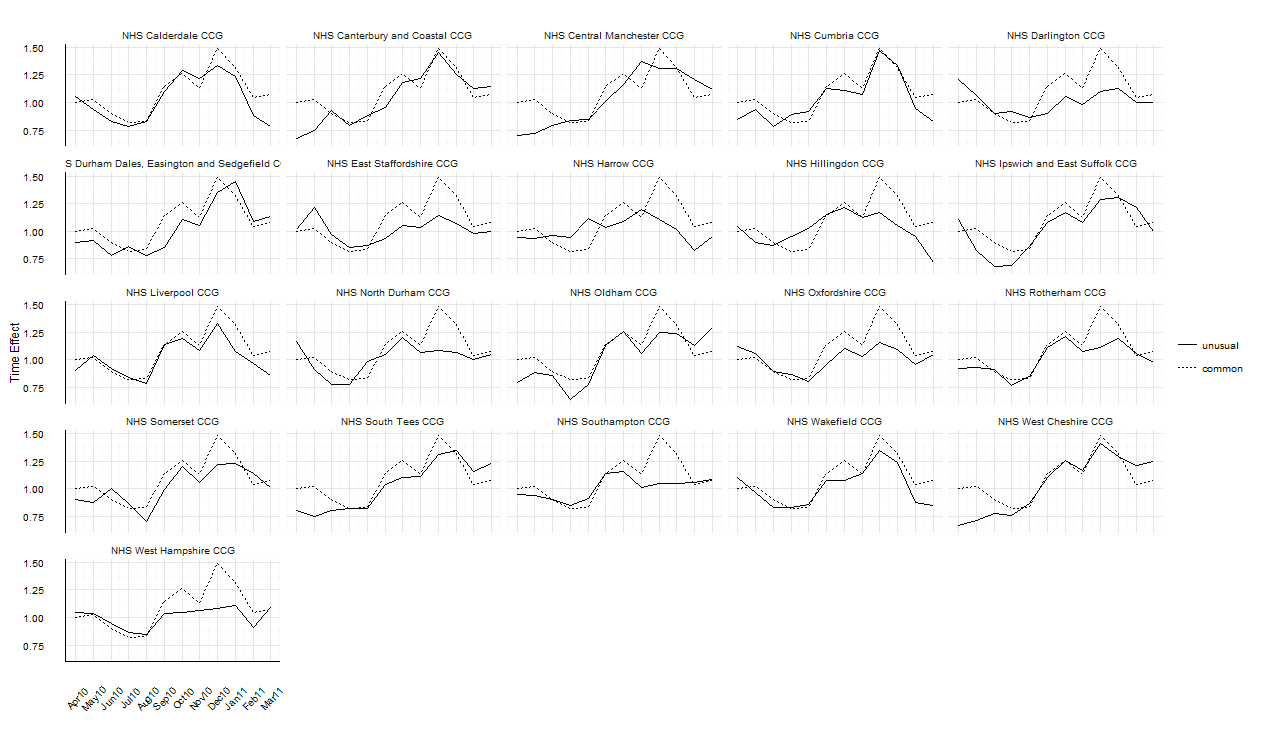
\includegraphics[height=6.8cm]{time_all.png}}}};
  \pause
  \node (img2) at (0,-1.7) {{\visible<2-2>{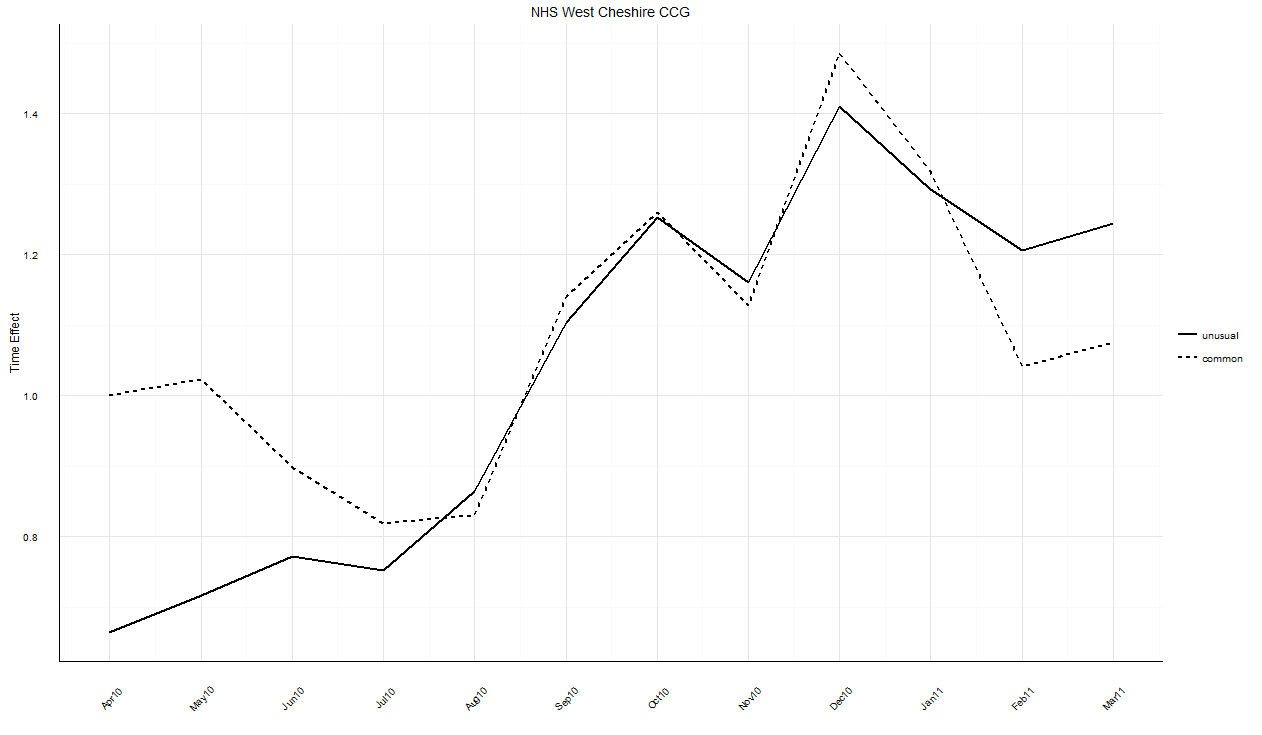
\includegraphics[height=5cm]{Cheshire.png}}}};
  \pause
 \node (img3) at (0,-2.7){{\visible<3-3>{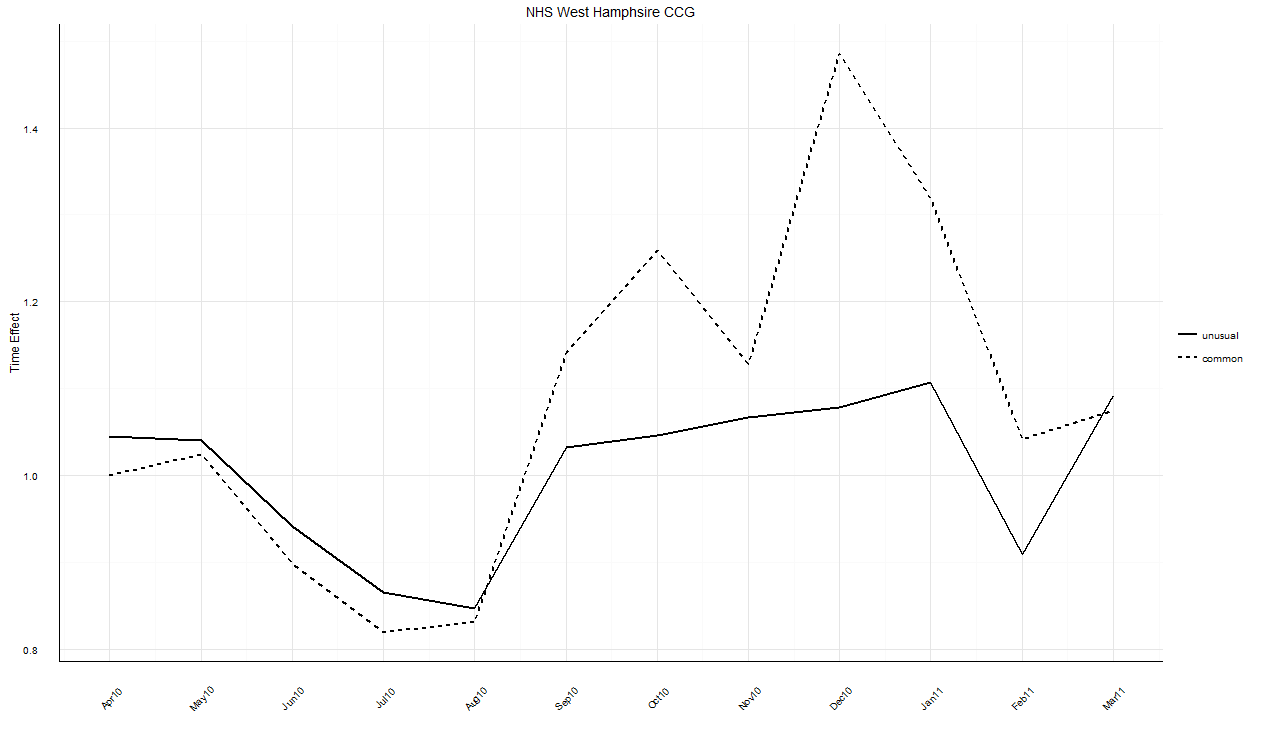
\includegraphics[height=5cm]{Hamphsire.png}}}};
 \pause
  \node (img4) at (0,-3.7) {{\visible<4-4>{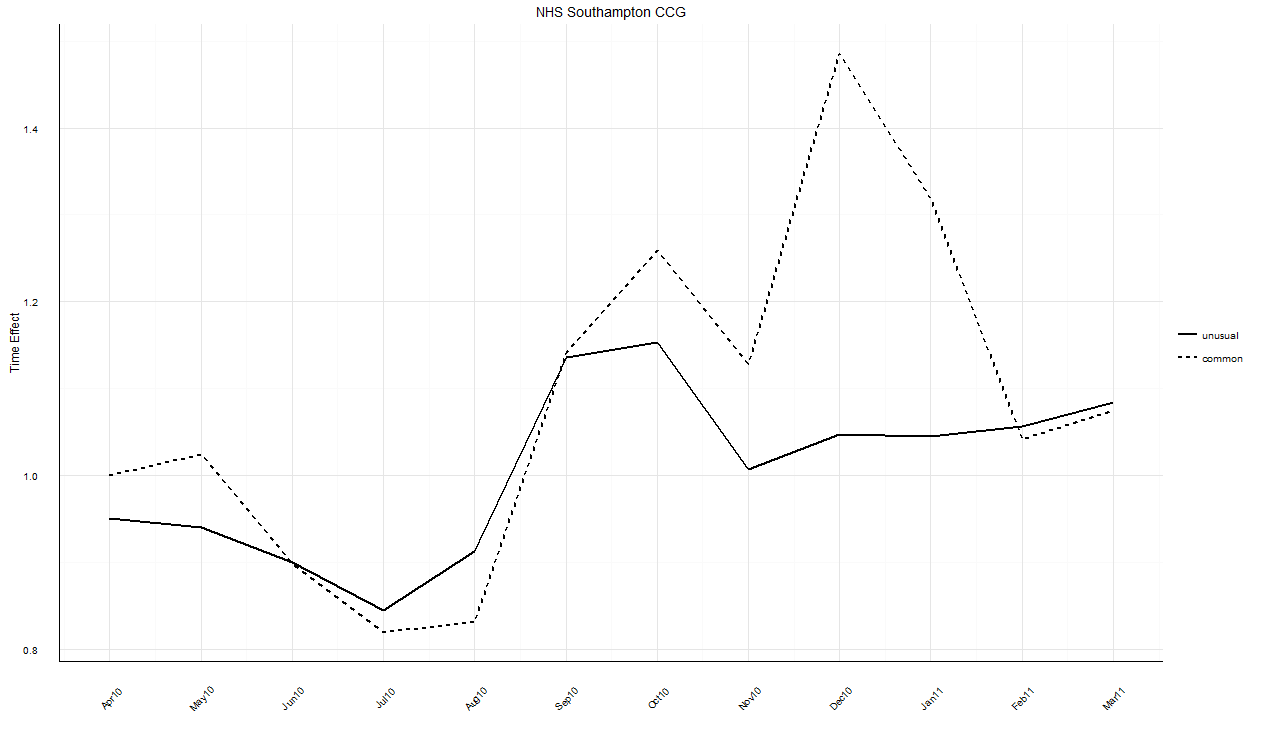
\includegraphics[height=5cm]{Southampton.png}}}};
 \pause
  \node (img5) at (0,-4.7) {{\visible<5-5>{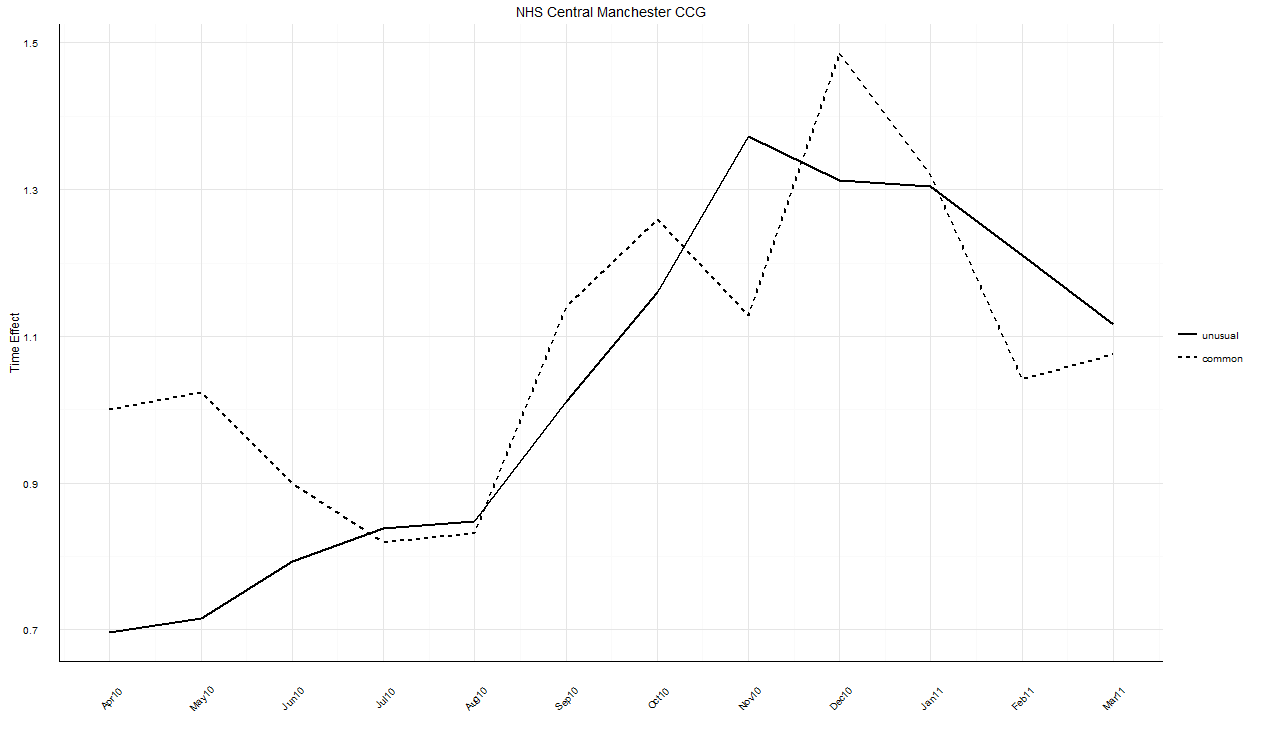
\includegraphics[height=5cm]{Manchester.png}}}};
  
\end{tikzpicture}
%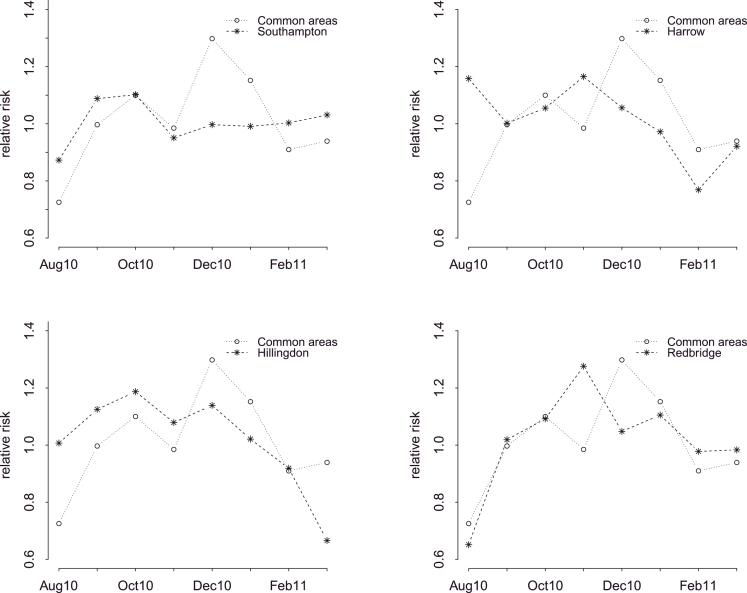
\includegraphics[scale=1.8]{gr4}
\end{center}

\vspace{200pt}\fontsize{7}{7}\selectfont{
Boulieri A, et al. ``Investigating trends in asthma and COPD through multiple data sources: A small area study'', \textbf{Spatial and SpatioTemporal Epidemiology}, 2016, 19: 28-36.}

\vspace{5pt}
\fontsize{7}{7}\selectfont{
Boulieri A, et al., ``A Bayesian mixture modelling approach\\ for epidemiological surveillance'', submitted to \textbf{Biostatistics}
}
\end{frame}
%%%%%%%%%%%%%%%%%%%%%%%%%%%
\begin{frame}
\frametitle{Example: Childhood leukaemia and benzene}
\begin{itemize}
\vfill\item Bayesian Disease mapping used to study leukaemia incidence in children. 
\vfill\item Can we explain some of the variation in risk of leukaemia by
environmental exposure to benzene?
\vfill\item Let $X_i$ = average benzene
emissions (tonnes per annum) in ward $i$.
\end{itemize}
\scalebox{0.5}{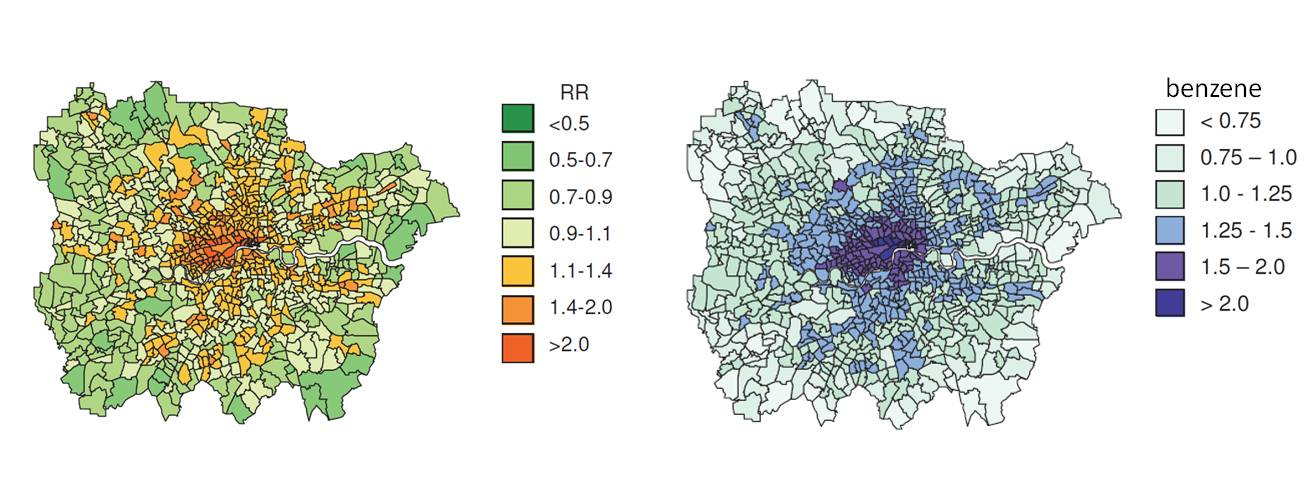
\includegraphics{leuk_benzene.jpg}}\\
 \end{frame}
%%%%%%%%%%%%%%%%%%%%%%%%%%%%%%%%%%%%%%%%%%%%%%%%%%%%%%%
\begin{frame}[t]
\frametitle{Maps of leukaemia RR}
\begin{itemize}\item Disease mapping to ecological regression. \end{itemize}
\begin{eqnarray*}
\log \lambda_{i} & = & \alpha + u_i + v_i + \beta X_i\\
\end{eqnarray*}
Relative risk of leukaemia associated with living in area with
benzene emissions in the top quartile compared to an area with
emissions in the bottom quartile = 1.29 (1.17, 1.41)
\begin{center}
\scalebox{0.35}{
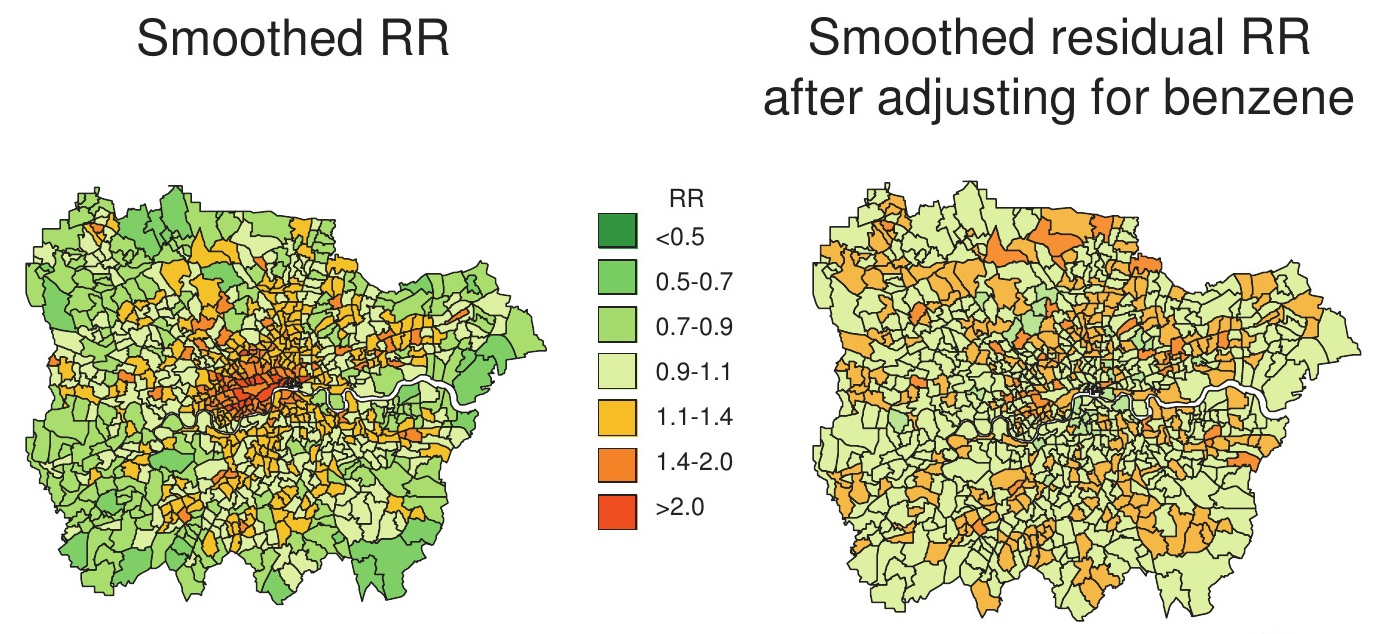
\includegraphics{leuk-maps-adjrr.jpeg}}\end{center}

\vspace{10pt}\fontsize{7}{7}\selectfont{Best, N. et al. (2001). ``Ecological regression analysis of environmental benzene exposure and childhood leukaemia: sensitivity to data inaccuracies, geographical scale and ecological bias''. \textbf{Journal of the Royal Statistical Society, Series A}, 164, 155-74.}
\end{frame}
%%%%%%%%%%%%%%%%%%%%%%%%%%%%%%%%%%%%%%%%%%%%%%%%%%%%%%%%%%%%%%%%%%%%%%%%%%%%%%%%%%%%%%%%
\begin{frame}
\frametitle{Example: Mortality Effects of Warm Temperature across Communities}
%\begin{itemize}
%  \item Investigate spatial patterns of temperature response for cardio-respiratory mortality across the 376 districts of England and Wales.
%\vspace{10pt}  \item Assess the presence of individual characteristics which lead to differences in the spatial patterns.
%\end{itemize}
%
%\begin{itemize}
%  \item Modification of case-control study: each case serves as their own control.
%  \item Control days fall on the same day of the week and in the same calendar month.
%  \pause\item The temperature on the day on which the i-{th} individual dies (case day) is compared with either 3 or 4 control days.\\ \begin{center}
%  $|$- - - C - - - - - - D - - - - - - C - - - - - - C - - - - -$|$\\
%  $|$- C - - - - - - C - - - - - - D - - - - - - C - - - - - - C$|$\end{center}
%  \pause \vspace{5pt}\item Analysed using conditional logistic regression.
%  \end{itemize}
%  
%\end{frame}
%
%
%%%%%%%%%%%%%%%%%%%%%%%%%%%%%%%%%%%%%%%%%%%%%%%%%%%%%%%%%%%%%%%%%%%%%%%%%%%%%%%%%%%%%%%%%
%\begin{frame}\frametitle{Model specification: first level}
\begin{itemize}
\item Investigate spatial patterns of temperature response for cardio-respiratory mortality across the 376 districts of England and Wales.
%\vspace{10pt}  \item Assess the presence of individual characteristics which lead to differences in the spatial patterns.
\end{itemize}  
Case-crossover design - for individual $i$, case/control $j$:
\begin{eqnarray*}
  O_{ij}&\sim& \text{Poisson}(\lambda_{ij})\\
  \log(\lambda_{ij}) &= &\text{f}(\beta_{0}, \beta_{1\text{dist}_i}, \text{Temp}_{ij}) + \delta_i + \text{C}_{ij}
\end{eqnarray*}

\begin{itemize}
\item $O_{ij}= 1$ for cases ($j=1$) and 0 for controls ($j=2,\ldots,J_i$);
\item $\delta_i$ links cases and controls from the same individual $i$;
\item $\beta_{0}$ is the threshold parameter for temperature response;
\item $\beta_{1\text{dist}_i}$  is the supra-threshold slope parameter.
\end{itemize}

\vspace{10pt} Confounders are
\[\text{C}_{ij} = \beta_{\text{PM}_{10}}\text{PM}_{10ij}  + \beta_{\text{Holiday}}\text{Holiday}_{ij}\]
\end{frame}

%%%%%%%%%%%%%%%%%%%%%%%%%%%%%%%%%%%%%%%%%%%%%%%%%%%%%%%%%%%%%%%%%%%%%%%%%%%%%
\frame{\frametitle{Bayesian Model: temperature model}\vfill
\begin{tabular}{cc}
\begin{minipage}{8cm}
The temperature threshold model \\
f$(\beta_{0},\beta_{1\text{dist}_i}, \text{Temp}_{ij})$ is:
\begin{eqnarray*}
0 && \text{ if Temp$_{ij}\leq \beta_{0}$} \\
\beta_{1\text{dist}_i}(\text{Temp}_{ij} - \beta_{0}) && \text{ if Temp$_{ij}> \beta_{0}$}
\end{eqnarray*}
\end{minipage}

&

\begin{minipage}{6.5cm}
\vspace{10pt}\scalebox{0.35}{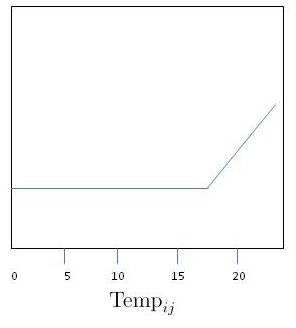
\includegraphics{SlopePlot.jpg}}
\end{minipage}
\end{tabular}

\pause\begin{itemize}
\item Fixed nationwide threshold.
%\item Deviance Information Criterion (DIC) is used to choose the best threshold parameter.
\item District specific supra-threshold slope parameter modelled via a combination of structured and unstructured random effects.
\item Stratified analysis for age classes and gender.
\end{itemize}
}
%%%%%%%%%%%%%%%%%%%%%%%%%%%%%%%%%%%%%%%%%%%%%%%%%%%%%%%%%%%%%%%%%%%%%%%%%%%%%%%%%%%%%%
%\frame{\frametitle{Nationwide Temperature Effect}\vfill
%
%Percent change in odds of death per 1C increase in mean daily temperature above threshold.
%\begin{center}\begin{small}
%\begin{tabular}{rrrc}
%\hline
%           &            &                & \% Change in odds of death (95\% CI)     \\
%           &        Age &     Deaths     &    per 1C                     \\
%\hline
%           &            &                &                               \\
%     Males &       < 75 &     71,436     & 2.9 (1.5,4.3)               \\
%           &      75 $-$ 84 &     75,207 & 2.1 (0.8,3.5)               \\
%           &       > 84 &     46,786 & 3.9 (2.2,5.6)                   \\
%\hline
%           &            &                &                               \\
%   Females &       < 75 &     38,536     & 2.6 (0.7,4.4)               \\
%           &      75 $-$ 84 &     74,999 & 4.3 (2.9,5.7)               \\
%           &       > 84 &     99,733     & 5.0 (3.8,6.1)               \\
%           &            &                &                                   \\
%\hline
%\end{tabular}
%\end{small}\end{center}
%}

%%%%%%%%%%%%%%%%%%%%%%%%%%%%%%%%%%%%%%%%%%%%%%%%%%%%%%%%%%%%%%%%%%%%%%%%%%%%%
\frame{\frametitle{Spatial Pattern of Temperature Effects in Females}\vfill
\only<1>{\begin{center}\vspace{-10pt}\begin{minipage}{10cm}
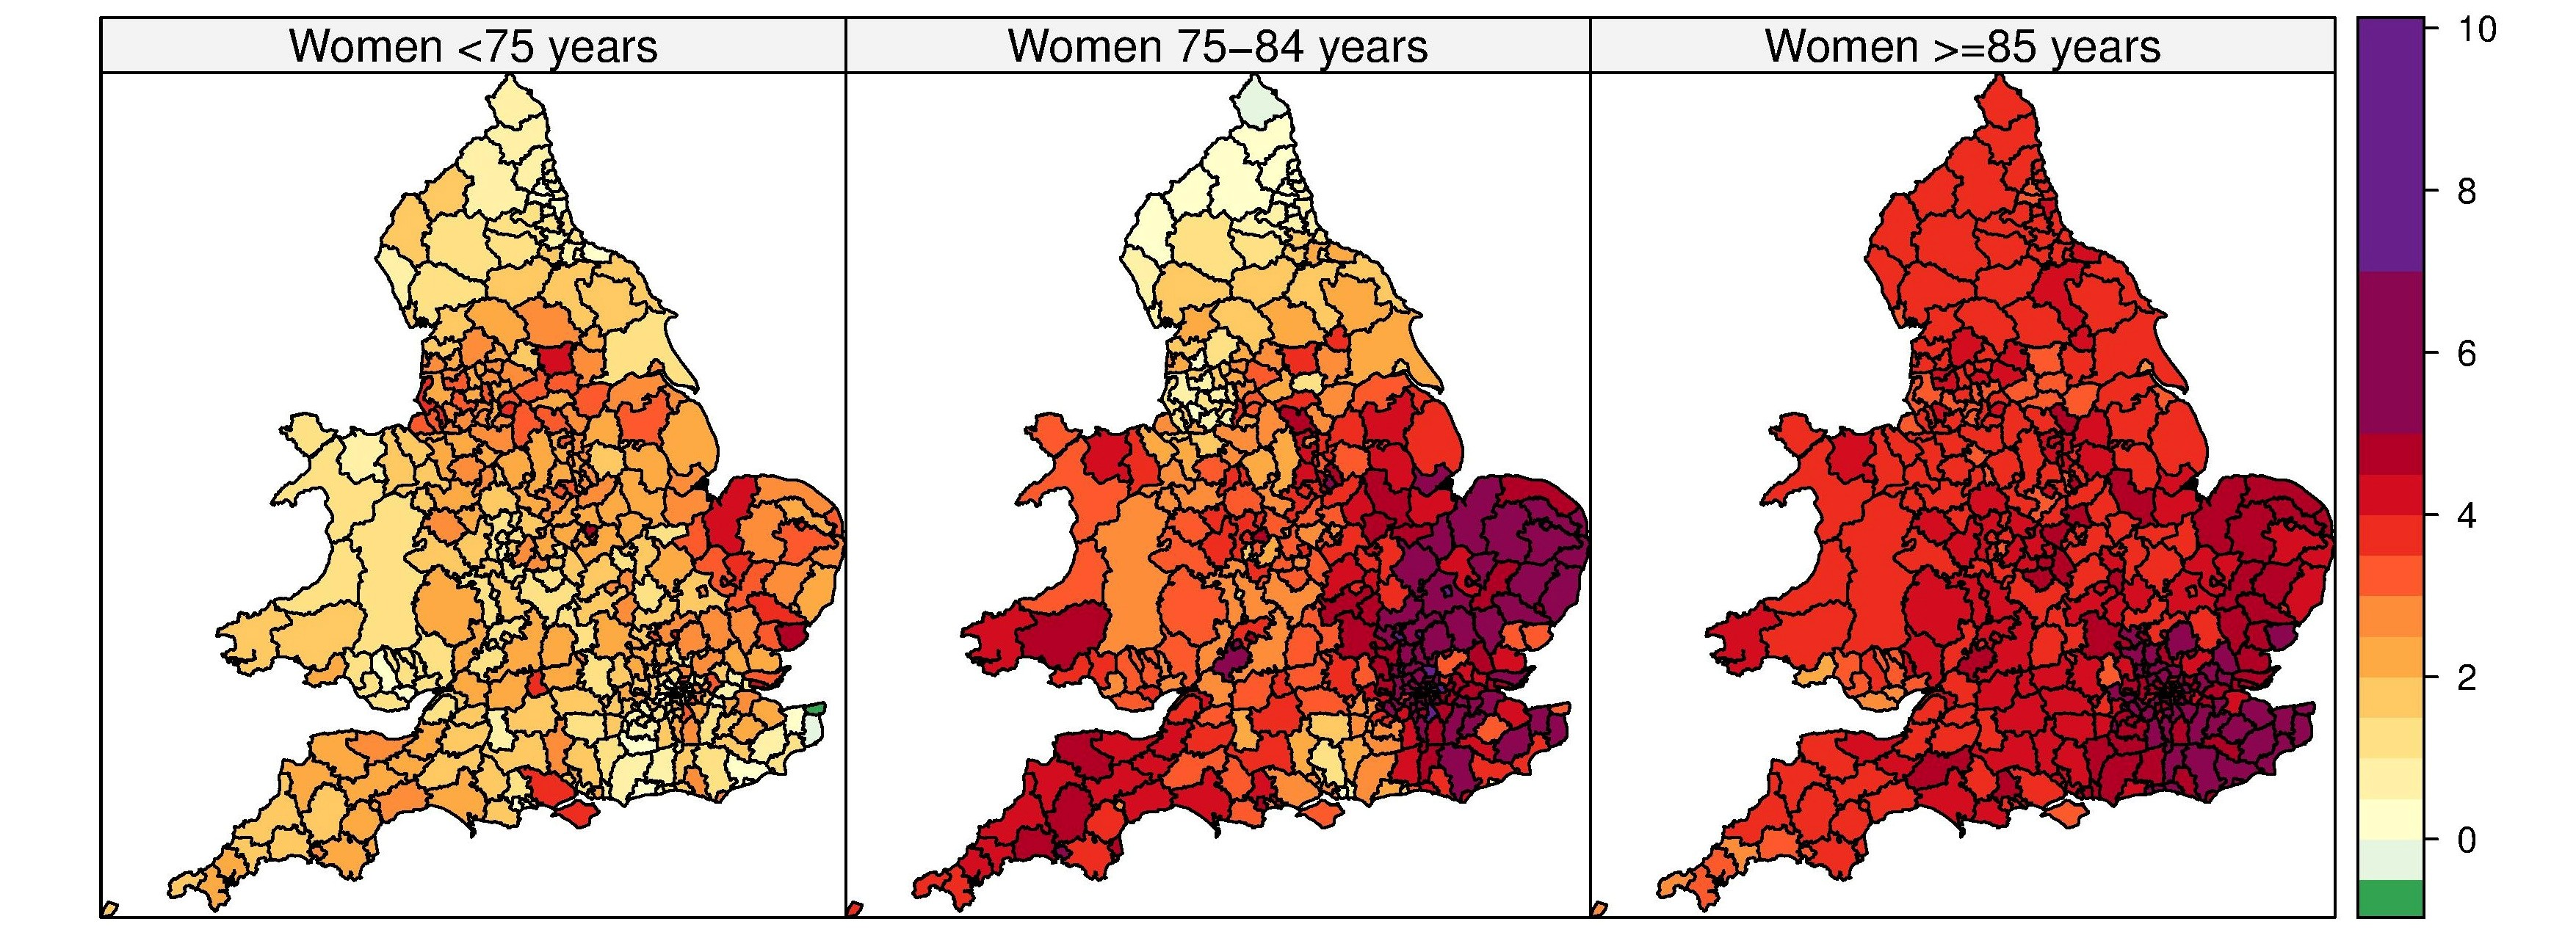
\includegraphics[width=10cm]{eMapSlopes_TH18_FgrpFont15.jpg}
\end{minipage}\end{center}

Consistent spatial pattern with age:

\begin{itemize}
  \item Higher \% increase in odds of death in the South.
  \item Consistent with other papers on the topic.
\end{itemize}
}

\only<2>{\begin{center}\vspace{-10pt}\begin{minipage}{10cm}
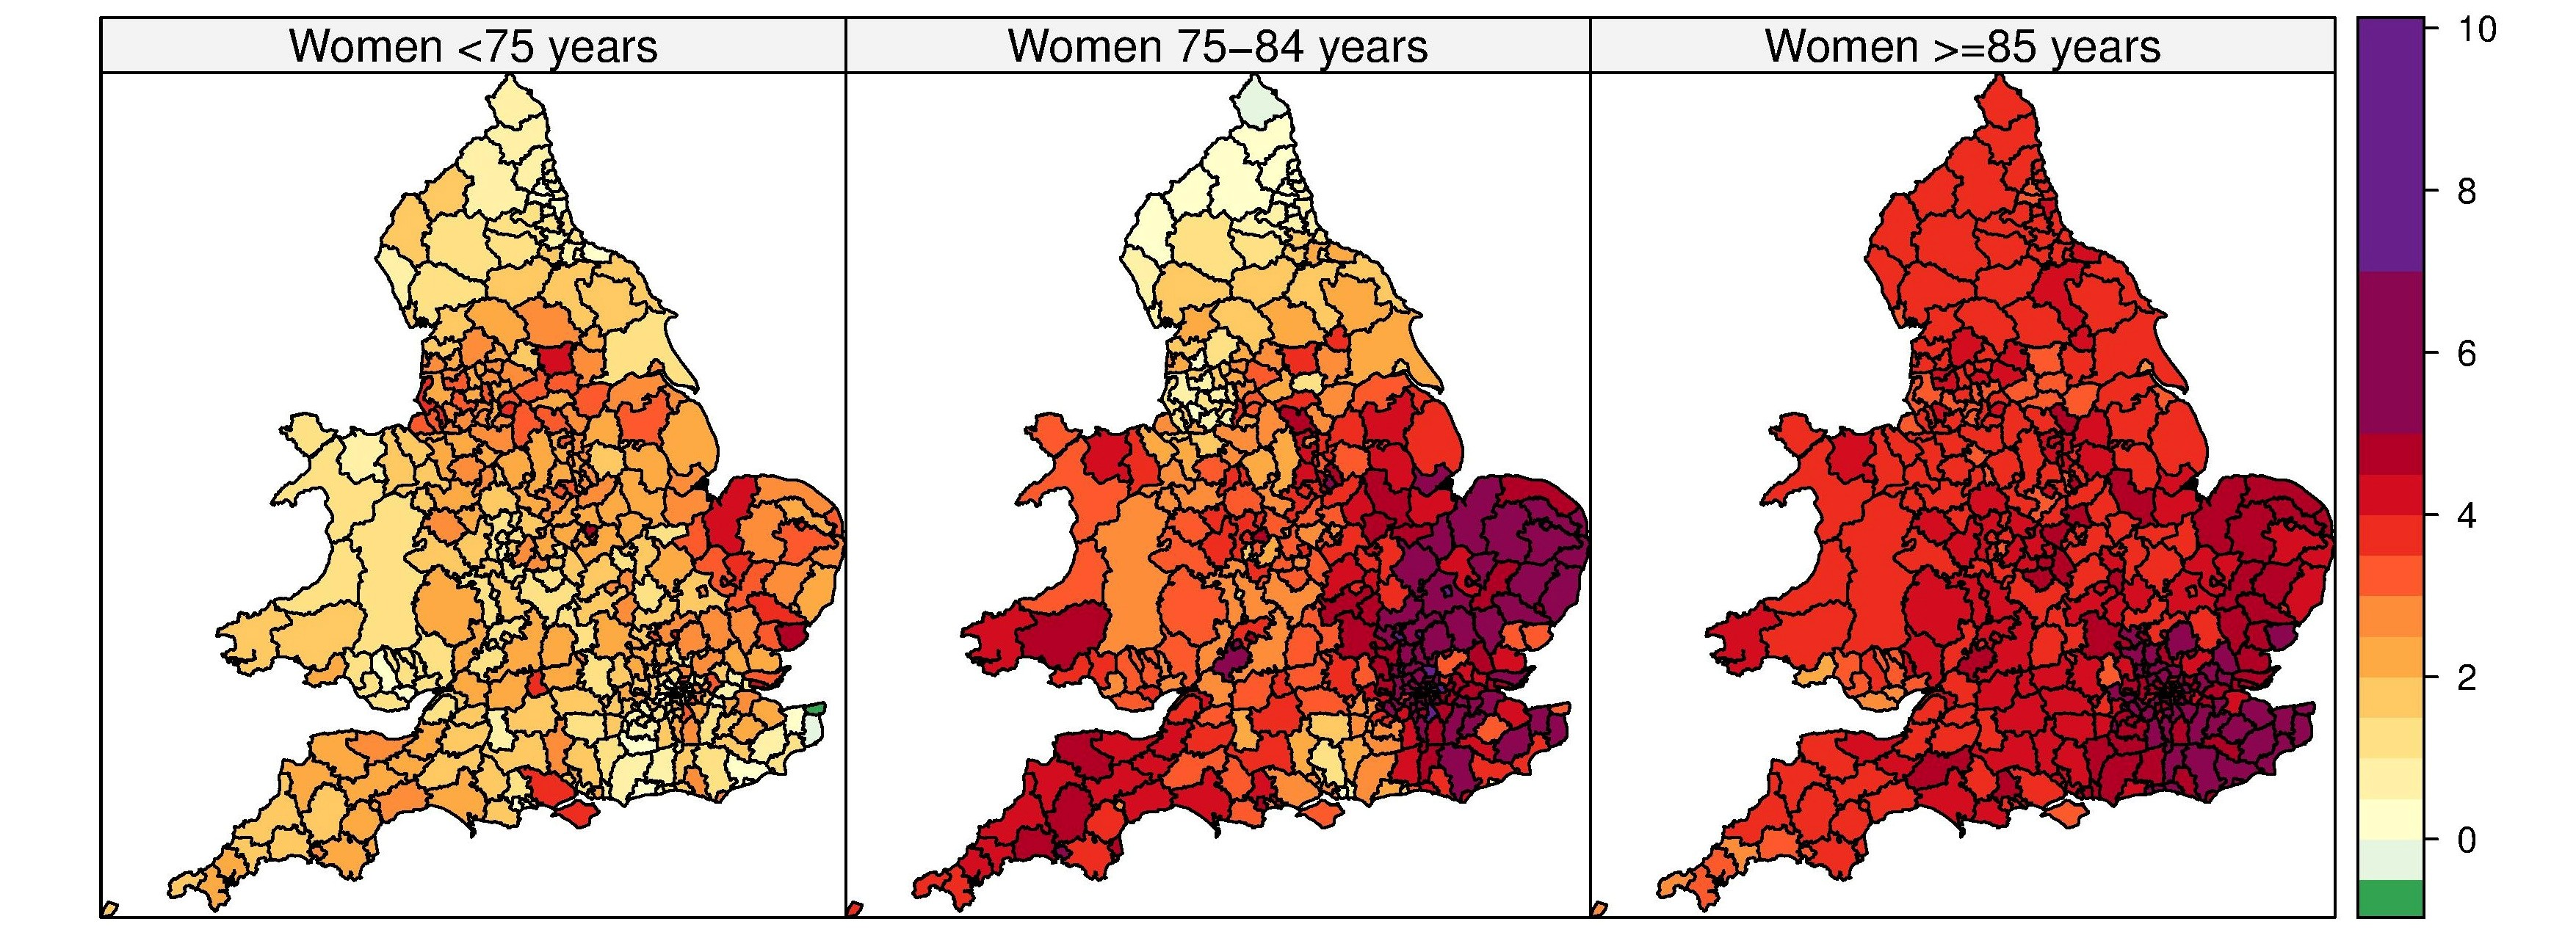
\includegraphics[width=10cm]{eMapSlopes_TH18_FgrpFont15.jpg}
\end{minipage}\end{center}

\begin{center}\vspace{-13pt}\begin{minipage}{10cm}
\hspace{2pt}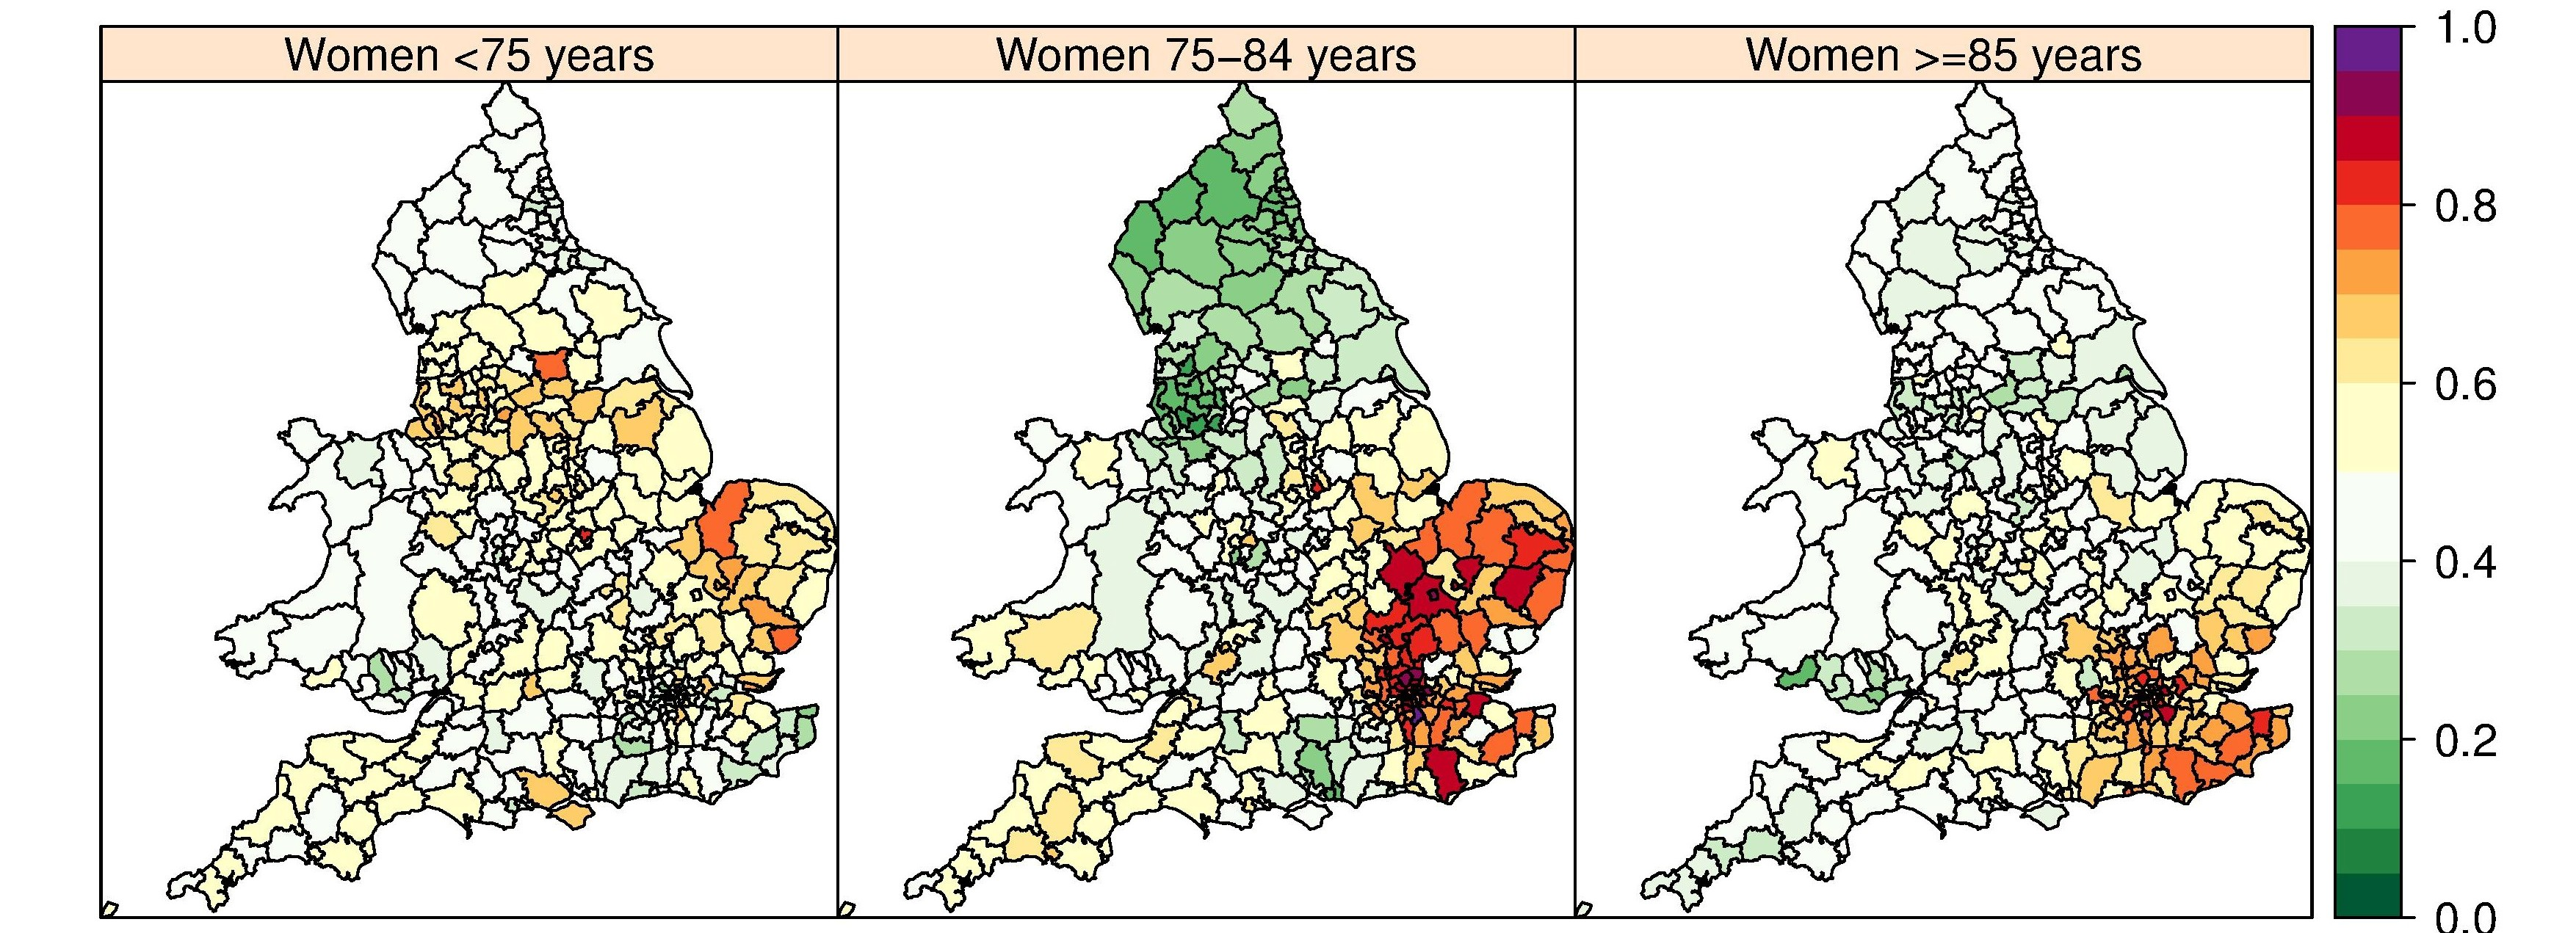
\includegraphics[width=10cm]{PP_gtA1_TH18_FdgrpFont15.jpg}
\end{minipage}\end{center}
}

\fontsize{7}{7}\selectfont{
Bennett J, et al., ``Vulnerability to the mortality effects of warm temperature in the districts of England and Wales'', \textbf{Nature Climate Change} 2014, 4, 269-273.}
}

%%%%%%%%%%%%%%%%%%%%%%%%%%%%%%%%%%%%%%%%%%%%%%%%%%%%%%%%%%%%%%%%%%%%%%%%%%%%%%%%%%%%%%%%
\begin{frame}\frametitle{Recap: Small area framework}
\begin{itemize}
\vfill\item Hierarchical Bayesian framework useful to deal with discrete spatial (temporal) data.
\vfill\item Disease mapping: To smooth the data and look for spatial and temporal patterns. 
\vfill\item Mixture models: To classify areas based on their temporal trends.
\vfill\item Regression models for risk assessment. 
\end{itemize}
\end{frame}
%%%%%%%%%%%%%%%%%%%%%%%%%%%%%%%%%%%%%%%%%%%%%%%%%%%%%%%%%%%%%%%%%%%%%%%%%%%%%%%%%%%%%%%%
%%%%%%%%%%%%%%%%%%%%%%%%%%%%%%%%%%%%%%%%%%%%%%%%%%%%%%%%%%%%%%%%%%%%%%%%%%%%%%%%%%%%%%%%
\section{Geostatistical framework}
\begin{frame}
\begin{center}
\vfill\fontsize{20}{20}\selectfont{Geostatistical framework}\end{center}
\end{frame}
%%%%%%%%%%%%%%%%%%%%%%%%%%%%%%%%%%%%%%%%%%%%%%%%%%%%%%%%%%%%%%%%%
\begin{frame}\frametitle{General inferential issues}
	Spatial (and temporal) pattern suggest that observations close to each other have more similar
	values than those far from each other.\\

\pause What are the aims of a geostatistical analysis?	
\begin{itemize}
\item Reconstruct a latent spatial (temporal) surface $\bm{S}$ from a finite set of noisy
observations and their spatial (temporal) location.
\item Use the spatial dependence to predict values of the spatial
surface (together with associated uncertainty) at locations where
there are no observations.\\
	$\rightarrow$ {\bf In this talk}: \alert{Spatial pattern of lymphatic filariasis disease}.
\end{itemize}	

\pause\vfill In addition: \begin{itemize}
\vfill\item Do we have to deal with different spatial resolution? \\ $\rightarrow$ Change of support.\\
	$\rightarrow$ {\bf In this talk}: \alert{Misalignment in air pollution study.}\\
\end{itemize}

\pause\vspace{10pt} The common framework to geostatistical models is that of Gaussian
random fields.
\end{frame}
%%%%%%%%%%%%%%%%%%%%%%%%%%%%%%%%%%%%%%%%%%%%%%%%%%%%%%%%%%%%%%%%%
\begin{frame}
\frametitle{Gaussian fields}
\begin{itemize}
\vfill\item A spatial process $y(\bm s)$ is a \alert{Gaussian field} (GF) if for any $n \geq 1$ and for each set of locations $(\bm s_{1},\ldots,\bm s_{n})$, the vector $\left(y(\bm s_1),\ldots, y(\bm s_n)
\right)$ follows a multivariate Normal distribution with mean $\bm \mu=\left(\mu(\bm s_{1}), \ldots, \mu(\bm s_{n})\right)$ and spatially structured covariance matrix $\bm \Sigma$. 
\vfill\item The  generic element of $\bm \Sigma$ is defined by a \alert{covariance function} $\mathcal C(\cdot,\cdot)$
 such that $\Sigma_{ij}=\mbox{Cov}\left(y(\bm s_{i}),y(\bm s_{j})\right)=\mathcal C(y(\bm s_{i}),y(\bm s_{j}))$.
\pause
\vfill\item The spatial process is called \alert{second-order stationary} if 
\begin{itemize}

\vfill\item $\bm \mu$ is constant (i.e. $\mu(\bm s_{i}) = \mu$ for each $i$) 
\vfill\item the spatial covariance function depends only on the distance vector $(\bm s_{i}-\bm s_{j}) \in \mathbb{R}^2$, i.e. $\mbox{Cov}\left(y(\bm s_{i}),y(\bm s_{j})\right)=\mathcal C(\bm s_{i}-\bm s_{j})$. 
\end{itemize}

\pause\vfill\item Moreover, a stationary process is \alert{isotropic} if the covariance does not depend on the direction but just on the Euclidean distance  $||\bm s_{i}-\bm s_{j}|| \in \mathbb{R}$.
\vfill\item[] Several functions are available for the spatial covariance function (eg exponential, Mat\'ern, spherical, etc.) parameterized by some parameters (eg spatial variance, range, etc.).
\end{itemize}
\end{frame}

%%%%%%%%%%%%%%%%%%%%%%%%%%%%%%%%%%%%%%%%%%%%%%%%%%%%%%%%%%
%\begin{frame}
%\frametitle{General framework}
%\begin{itemize}
%\vfill\item Space is continuous.
%\vfill\item The process of interest (response) is an underlying spatial field $\{S(\bm s), \bm s \in \mathcal D\}$, i.e. real values stochastic process characterized by a spatial index $\bm s$ which varies continuously in the fixed domain $\mathcal D$.
%\vfill\item Examples: 
%\begin{itemize}
%\vfill\item in the field of environmental science: rainfall, air pollution concentrations, radioactive emission in soil, etc.
%\vfill\item in epidemiology when considering the risk of disease at different locations.
%\end{itemize}
%\vfill\item Data are measured (possibly with error) at $n$ spatial locations $(\bm s_{1},\ldots,\bm s_{n})$ and are denoted by $\bm y=\left(y(\bm s_1),\ldots, y(\bm s_n)\right)=(y_1,\ldots,y_n)$.
%\end{itemize}
%\end{frame}
%%%%%%%%%%%%%%%%%%%%%%%%%%%%%%%%%%%%%%%%%%%%%%%%%%%%%%%%%%%%%%%%%%%%%%%%
\begin{frame}
\frametitle{Model for geostatistical data}
Data are measured (possibly with error) at $n$ spatial locations $(\bm s_{1},\ldots,\bm s_{n})$ and are denoted by $\bm y=\left(y(\bm s_1),\ldots, y(\bm s_n)\right)=(y_1,\ldots,y_n)$.

Usually the following model is assumed
\[
y(\bm s) = \mu(\bm s) + \xi(\bm s) +\epsilon(\bm s)
\]
 where
\begin{itemize}

\item $\mu(\bm s)$  is the so-called large scale component, defined by some covariates.
\item $\xi(\bm s)$  is a zero mean Gaussian spatial process commonly assumed to be stationary and isotropic with covariance function $Cov(\xi(\bm s_i),\xi(\bm s_j))$  which depends only on the distance between the locations.
\item $\epsilon (\bm s)$  represents the measurement error and its variance is usually known as nugget effect.
\end{itemize}

\end{frame}

%%%%%%%%%%%%%%%%%%%%%%%%%%%%%%%%%%%%%%%%%%%%%%%%%%%%%%%%%%%%%%%%%%%%%%%%

\begin{frame}
\frametitle{Mat\`ern covariance function}
\vspace{-0.5cm}
\[
\text{Cov}(\xi(\bm s_i),\xi(\bm s_j))= \text{Cov}(\xi_i,\xi_j)=\frac{\sigma^2}{\Gamma(\lambda)2^{\lambda-1}}\left(\kappa ||\bm s_i - \bm s_j||\right)^\lambda K_\lambda\left(\kappa ||\bm s_i - \bm s_j||\right)
\]
where
\begin{itemize}

\item  $||\bm s_i - \bm s_j||$  is the Euclidean distance between two generic locations $\bm s_i, \bm s_j \in \mathbb{R}^d$
\item $\sigma^2$  is the \alert{variance}
\item $K_\lambda$  denotes the modified Bessel function of second kind and order $\lambda>0$, which measures the degree of \alert{smoothness} of the process. 
\item $\kappa>0$  is a \alert{scale} parameter related to the range $r$, i.e.\ the distance at which the spatial correlation becomes almost null. 
%Typically, the empirically derived definition for the range is
%$r=\frac{\sqrt{8 \lambda}}{\kappa}$, with $r$  corresponding to the distance at which the spatial correlation is close to 0.1, for each $\lambda\geq 1/2$.

\begin{center}\begin{tabular}{cc}
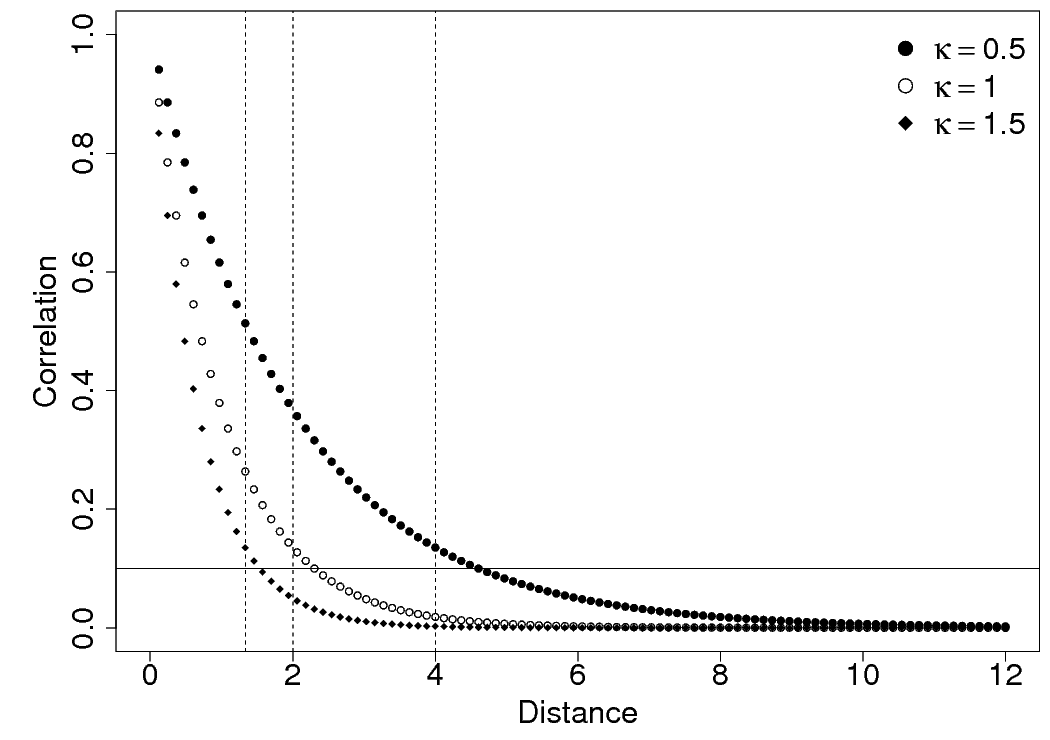
\includegraphics[scale=0.15]{Matern1} & 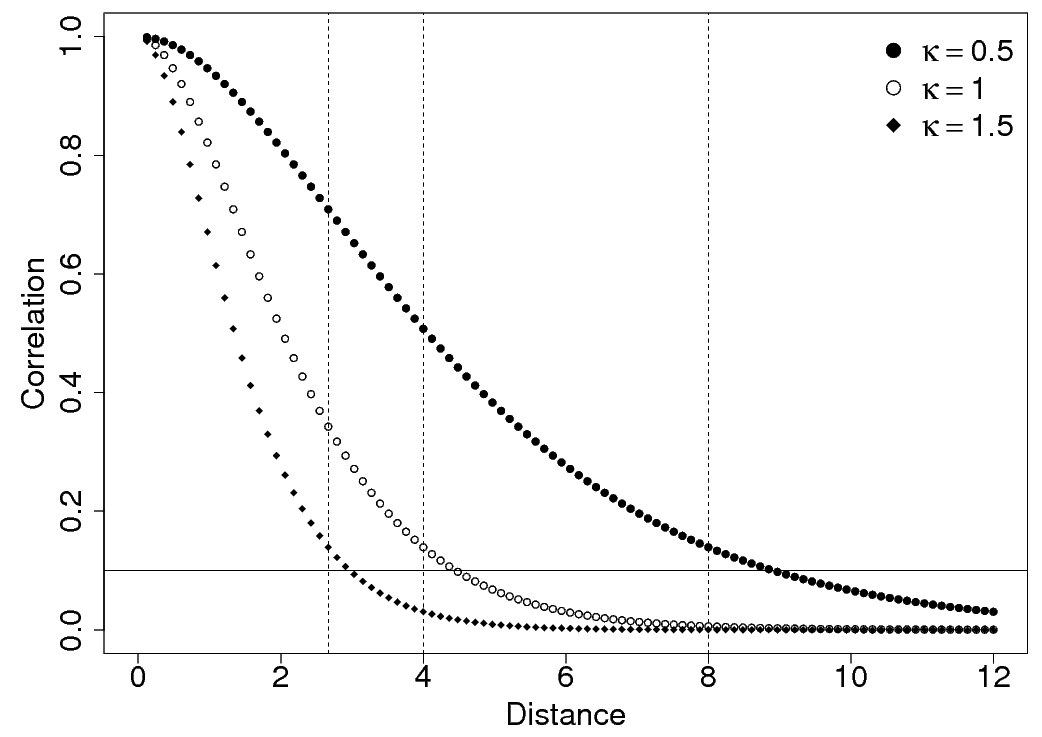
\includegraphics[scale=0.15]{Matern2}
\end{tabular} \end{center}

\item  The Mat\'ern family is a very flexible class of covariance functions able to cover a wide range of
spatial fields.
\end{itemize}
\end{frame}
%%%%%%%%%%%%%%%%%%%%%%%%%%%%%%%%%%%%%%%%%%%%%%%%%%%%%%%%%%%%%%%%%%%%%%%%
\frame{\frametitle{Variogram}
\begin{itemize} 
\item In order to explore the decay of the spatial covariance with distance, empirical plots are useful
\item The {\red empirical variogram}
is a tool to visualise spatial correlation. Given a
variable $y(\bm{s})$ measured at a set of $n$ locations, the empirical (semi)-variogram
is defined as
$$ \gamma_{ij} = \frac{1}{2}(y(\bm{s}_i) - y(\bm{s}_j))^2; \qquad\qquad i,j=1,\ldots,n$$
\item Values of $ \gamma_{ij}$ are then plotted against the distances between $\bm{s}_i$ and $\bm{s}_j$ for every pair of locations to produce a {\textcolor{red}{variogram cloud}}.
\item To aid interpretation the empirical variogram is often computed by averaging  $\gamma_{ij}$ within distance bands.
%\item It can be computed by using the function {\tt variog} in the package {\tt geoR} (Ribeiro and Diggle, 2006).
\end{itemize}
}

%%%%%%%%%%%%%%%%%%%%%%%%%%%%%%%%%%%%%%%%%%%%%%%%%%%
\frame{\frametitle{Variogram for the rain fall in Brazil example (15 (left) or 20 (right) distance classes)}
\begin{center}\vspace{-0.2cm}\rotatebox{0}{\scalebox{0.3}{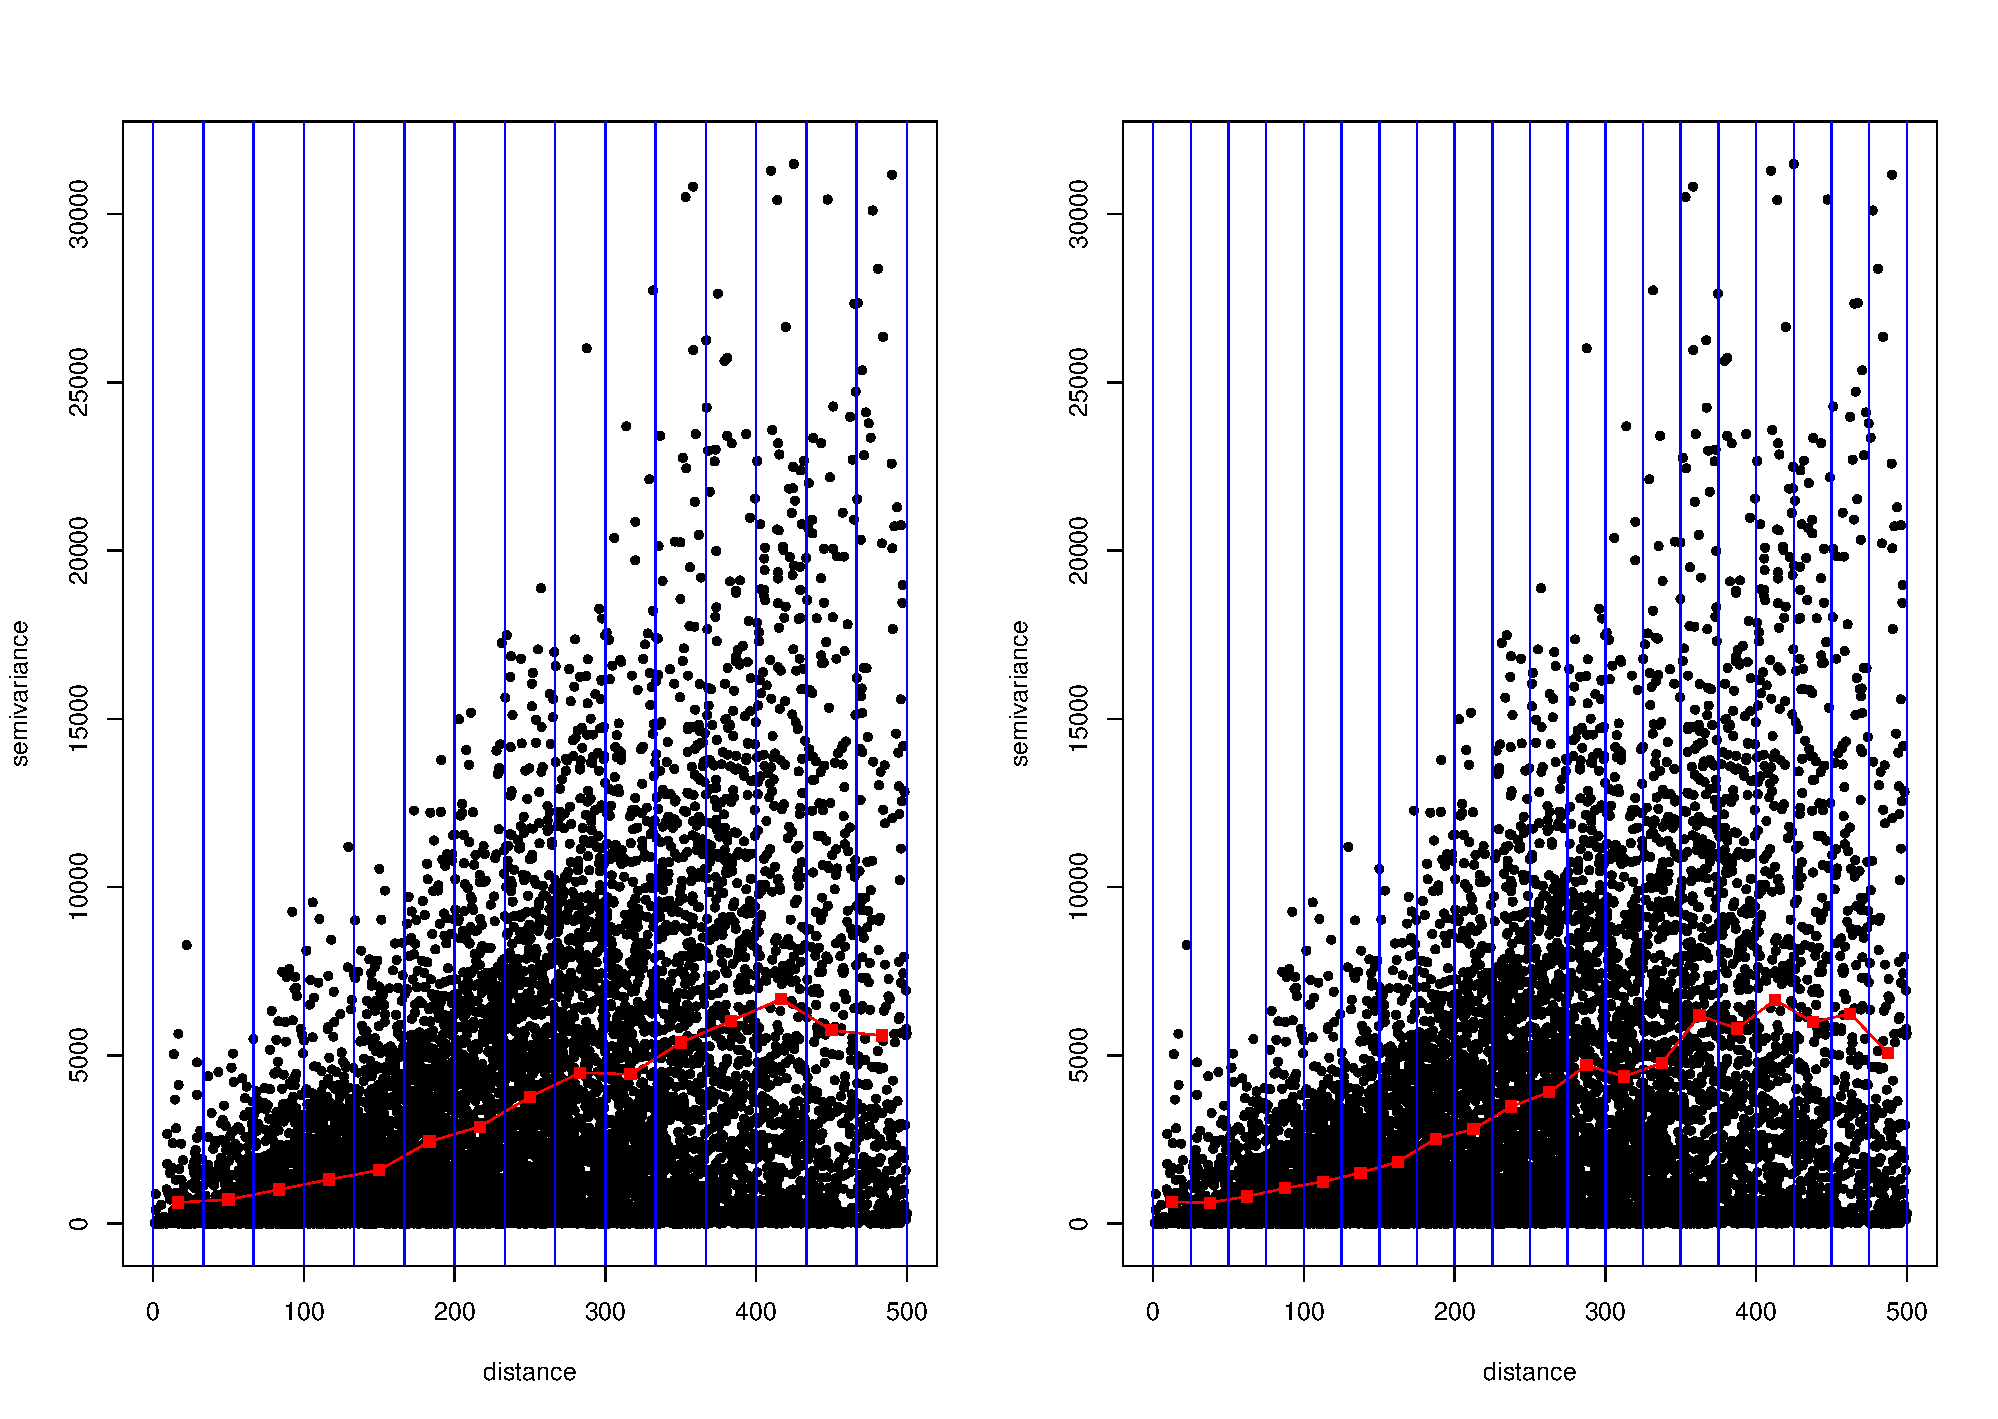
\includegraphics{variogram_parana_truncated}}}\end{center}
}
%%%%%%%%%%%%%%%%%%%%%%%%%%%%%%%%%%%%%%%%%%%%%%%%%%%%
\frame{\frametitle{Interpreting the Variogram}
\begin{itemize}
\vfill\item The variogram measures half the squared difference between each pair of locations.
\vfill\item If the data are spatially correlated, we would expect observations close together to be more similar than observations far apart (squared differences for observations close together will be smaller than for observations further apart so expect the variogram to gradually increase with increasing distance between observations).
\vfill\item If data are independent, then on average we would expect the squared difference of a pair of observations that are close together to be similar to that of observations further apart (variogram should be approximately constant as distance increases).
\end{itemize}
}
%%%%%%%%%%%%%%%%%%%%%%%%%%%%%%%%%%%%%%%%%%%%%%%%%%%%%%%%%%%%%%%%%%%%%%%%
\begin{frame}
\frametitle{Possible approaches for estimation}
\begin{itemize}

\vfill\item \alert{Classical geostatistical approach}: the empirical variogram is used as an exploratory tool and the mean and the covariance function parameters are estimated through  least square methods usually adopting a two step procedure\\ 
$\rightarrow$  very simple and not computationally intensive;\\
%$\rightarrow$  restrictive in the models that can accommodate;\\
$\rightarrow$  two-step approach to prediction;\\
$\rightarrow$  difficult to account for uncertainty. 

\pause
\vfill\item \alert{(Bayesian) Model-based}  \alert{approach}:  hierarchical model specification and posterior predictive distribution for prediction;\\
$\rightarrow$  easy to allow for uncertainty;\\
$\rightarrow$  flexible in accounting for any type of distribution;\\
$\rightarrow$ high computationally costs, especially for factorizing the spatial covariance matrix $\bm \Sigma$ (this is known as ``big $n$ problem'').
\end{itemize}

%\pause
%\vfill\item \alert{The stochastic partial differential equation (SPDE) approach} proposed by \cite{Lindgren:2011}: it represents a continuous spatial process $\xi(\bm s)$  with Mat\'ern covariance function using a discretely indexed spatial random process (ie a GMRF),  which is characterized by a sparse precision matrix and enjoys computational benefits in terms of fast inference.
%
\end{frame}
%%%%%%%%%%%%%%%%%%%%%%%%%%%%%%%%%%%%%%%%%%%%%%%%%%%%%%%%%%%%%%%%%
\subsection{Examples}
\begin{frame}\frametitle{Example: Lymphatic filariasis in Africa}
\begin{itemize}
\item Lymphatic filariasis (LF) - major vector-borne parasitic
disease endemic to the tropics, including sub-Saharan Africa.
\item First pan-african spatial analysis of environmental factors of LF (altitude, temperature, rain, pop. density).
\item Bayesian approach - posterior predictive distribution to predict on a regular grid
\end{itemize}
%\begin{eqnarray*}
%p(y_{s^\star} \mid \bm{y}, x, x_{s^\star}) &=& \int p(y_{s^\star}, \boldsymbol{\theta}\mid y,x,x_{s^\star})d\theta\\
%&=& \int p(y_{s^\star}\mid \bm{y}, \boldsymbol{\theta}, x_{s^\star})p(\boldsymbol{\theta}\mid \bm{y},x)d\theta  
%\end{eqnarray*}
\begin{figure}[!h]
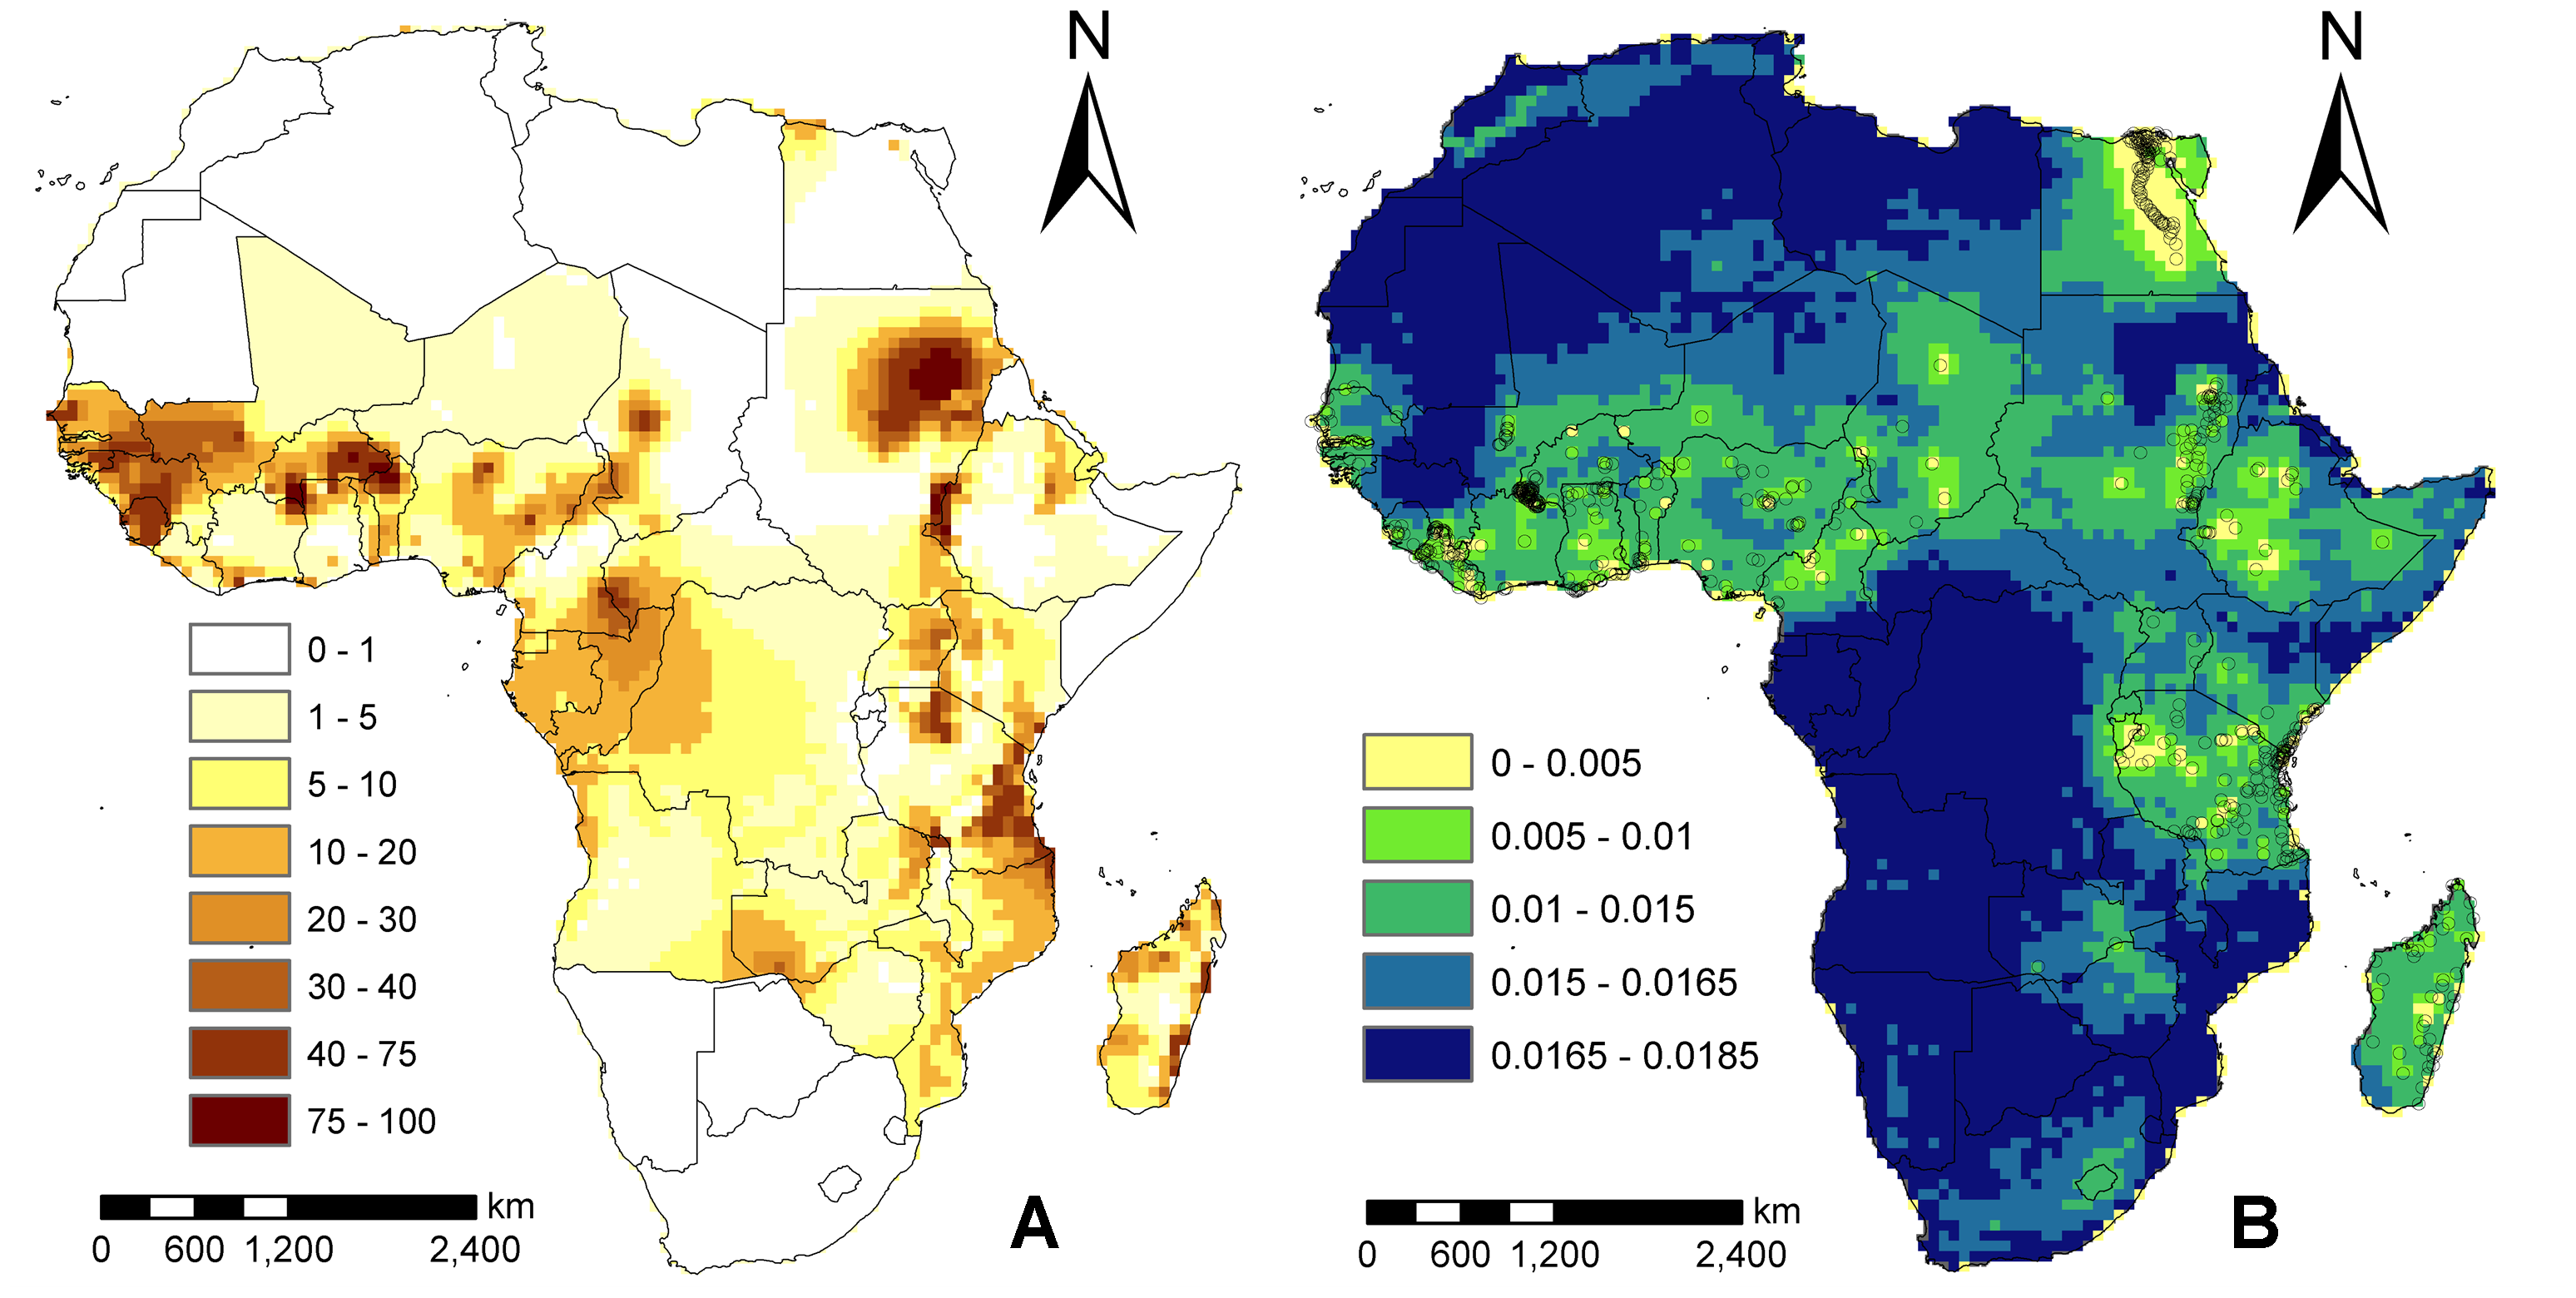
\includegraphics[scale=0.4]{journalpone0071574g004}\caption{A: Posterior mean of LF prevalence; B: Uncertainty estimate}   
\end{figure}
\fontsize{7}{7}\selectfont{Slater H, Michael E (2013) Mapping, Bayesian Geostatistical Analysis and Spatial Prediction of Lymphatic Filariasis Prevalence in Africa. PLoS ONE 8(8):e71574.}
\end{frame}
%%%%%%%%%%%%%%%%%%%%%%%%%%%%%%%%%%%%%%%%%%%%%%%%%%%%%%%%%%%%%%%%%
\begin{frame}
\frametitle{Example:Air pollution spatio-temporal exposure model}

$y(\bm s_{j},t)$: square root of air pollution concentration at  monitoring station located at site $\bm s_j$ ($j=1,\ldots, J$) and time $t=1,\ldots, T$. We assume:
\begin{eqnarray*}
y(\bm s_{j},t)  &=& \mu(\bm s_{j},t) + \omega(\bm s_{j},t) + \epsilon(\bm s_{j},t)\\
\mu(\bm s_{j},t)&=&b_0+ b_1\text{Temp}(\bm s_{j},t)+ b_2 \text{Baseline}(\bm s_{j})\\
\epsilon(\bm s_{j},t)&\sim& \text{Normal}(0, \sigma^{2}_{e})   
\end{eqnarray*}

where 
\begin{itemize}
\item<2-> $\omega(\bm s_{j},t) $ is a latent spatio-temporal process characterised by AR(1) temporal dynamics:
which changes in time with first order autoregressive dynamics with coefficient $a$ and spatially correlated innovations, given by
\[
\omega(\bm s_{j},t) =a \omega(\bm s_{j},t-1)  + \xi(\bm s_{j},t) \;
\]
with $\xi(\bm s_{j},t)$ being a zero-mean spatial continuous process with Mat\'ern covariance function.
\item<3-> $\mu(\bm s_{j},t) + \omega(\bm s_{j},t) = x(\bm s_{j},t)$ is the latent field.
\end{itemize}
\end{frame}
%%%%%%%%%%%%%%%%%%%%%%%%%%%%%%%%%%%%%%%%%%%%%%%%%%%%%%%%%%%%%%%%%%%%%%%%%%%%%%%%%%
\begin{frame}
\frametitle{Spatial prediction: $x(\bm s_{j},t) \leadsto x(\bm s_l^\star,t)$}
\begin{itemize}
\item  $x(\bm s_{j},t)$ are estimated through the model; 
\item To cover the spatial domain, for all the time points it is possible to sample from the posterior predictive distributions for each point $\bm s_l^\star$ in a regular grid. 
\end{itemize}
%(e.g. 690 grid points here).

\begin{center}
\begin{tikzpicture}[overlay]
  \node (img1) at (-2.5,-2.0) {{\visible<1->{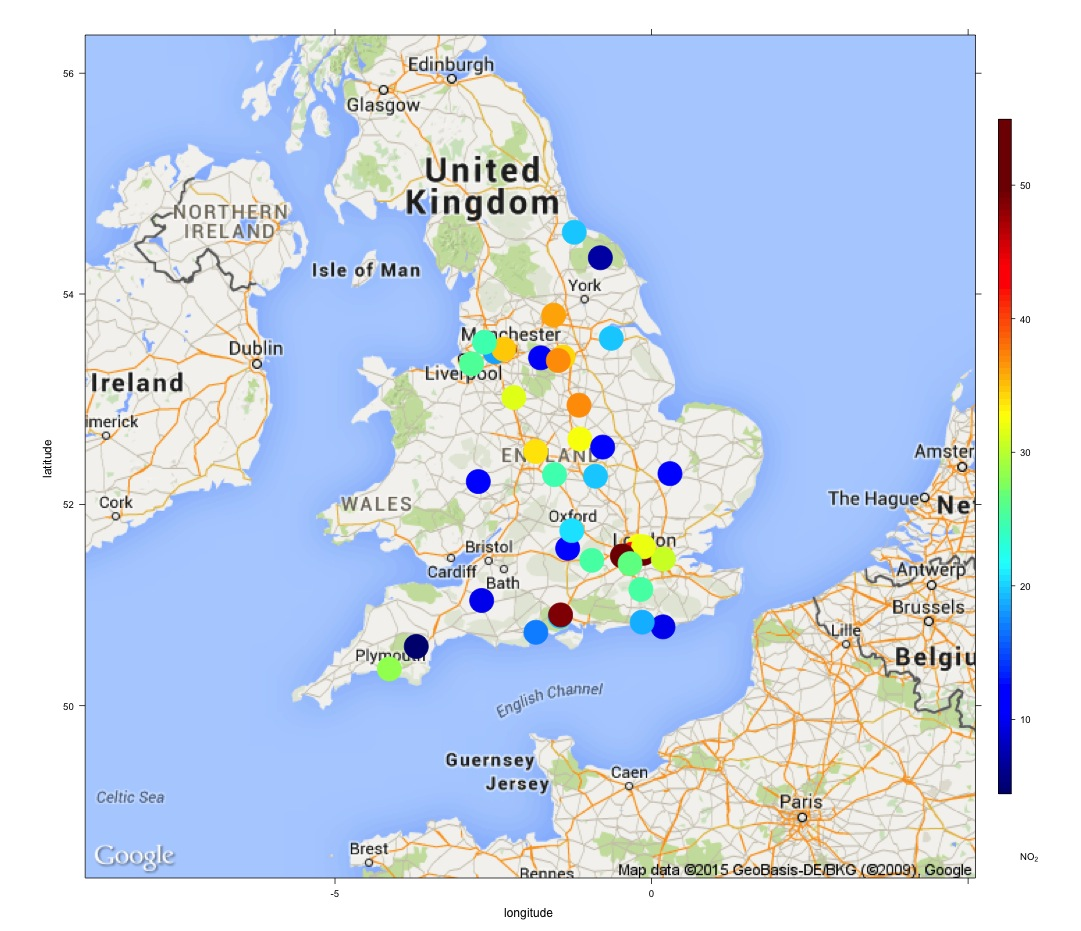
\includegraphics[scale=.15]{Map_NO2stations}}}};
  \pause
  \node (img2) at (2.6,-2.0) {{\visible<2-2>{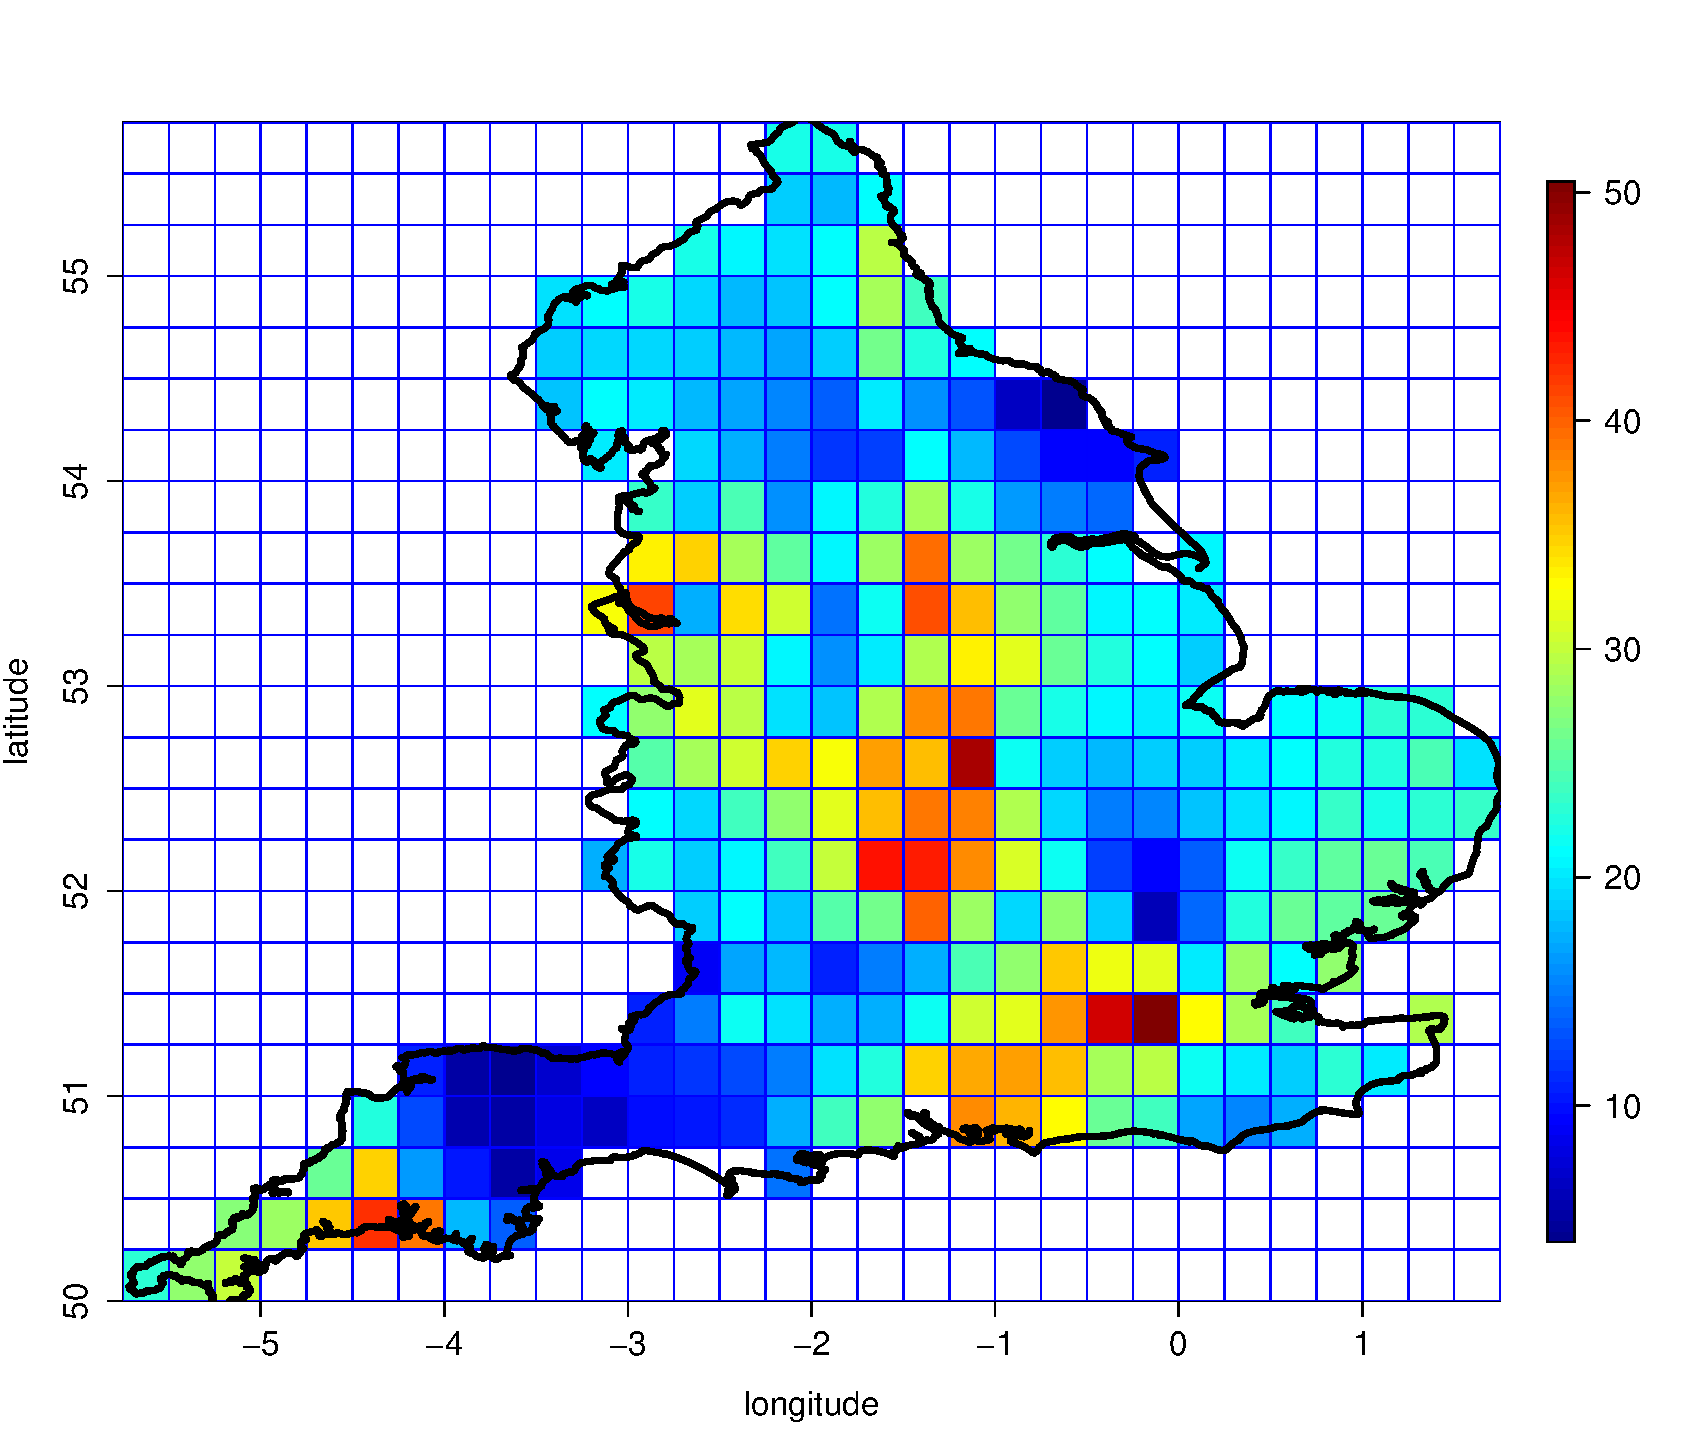
\includegraphics[scale=.2]{Month13_grid.pdf}}}};
\end{tikzpicture}
\end{center}
\end{frame}
%%%%%%%%%%%%%%%%%%%%%%%%%%%%%%%%%
\begin{frame}\frametitle{Change of support}
\begin{itemize}
\item<1-> Air pollutant concentrations available at monitoring stations in a study region, while disease data appear as counts observed in given areas.

\item<2-> \alert{\textit{Change of support}}:
\[
x_{it}=\int_{\bm s \in \mathcal A_i} x(\bm s,t) \; p(\bm s) \; d\bm s \approx \sum_{l=1}^{N_i} \textcolor{blue!80}{x(\bm s_{il}^\star,t)} \; p(\bm s_{il}^\star)
\]
 \small{where $x(\bm s_{ij}^\star,t)$ is the pollutant concentration prediction at location $s_{il}^\star$, one of $N_i$ \alert{regular grid points} inside area $\mathcal A_i$; moreover$ \sum_{l=1}^{N_i}p(\bm s_{il}^\star)=1$}.

\begin{center}
\begin{tabular}{ll}
\hspace{-1cm}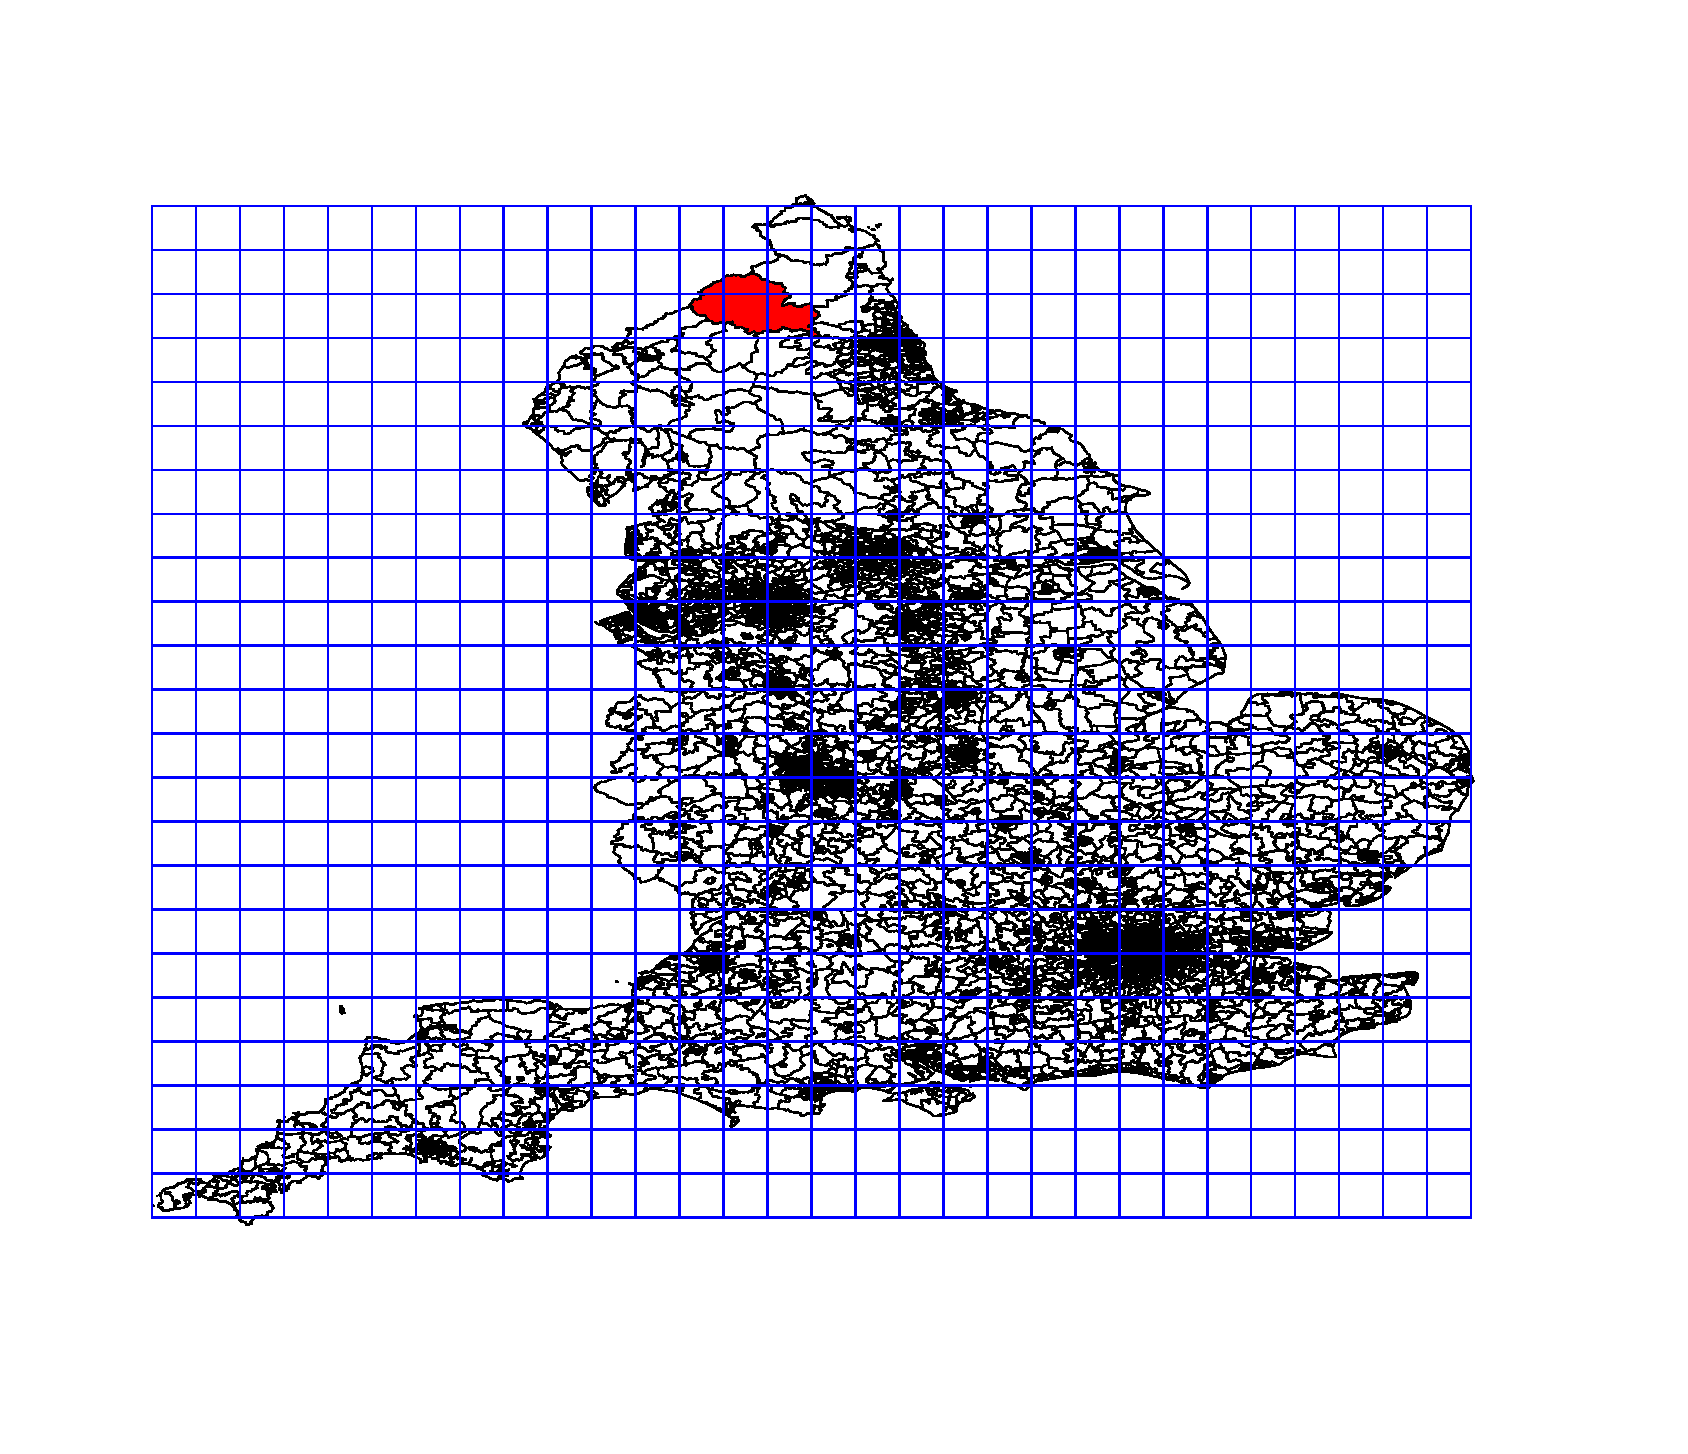
\includegraphics[scale=.15]{MSOA_grid.pdf} &\hspace{-0.75cm}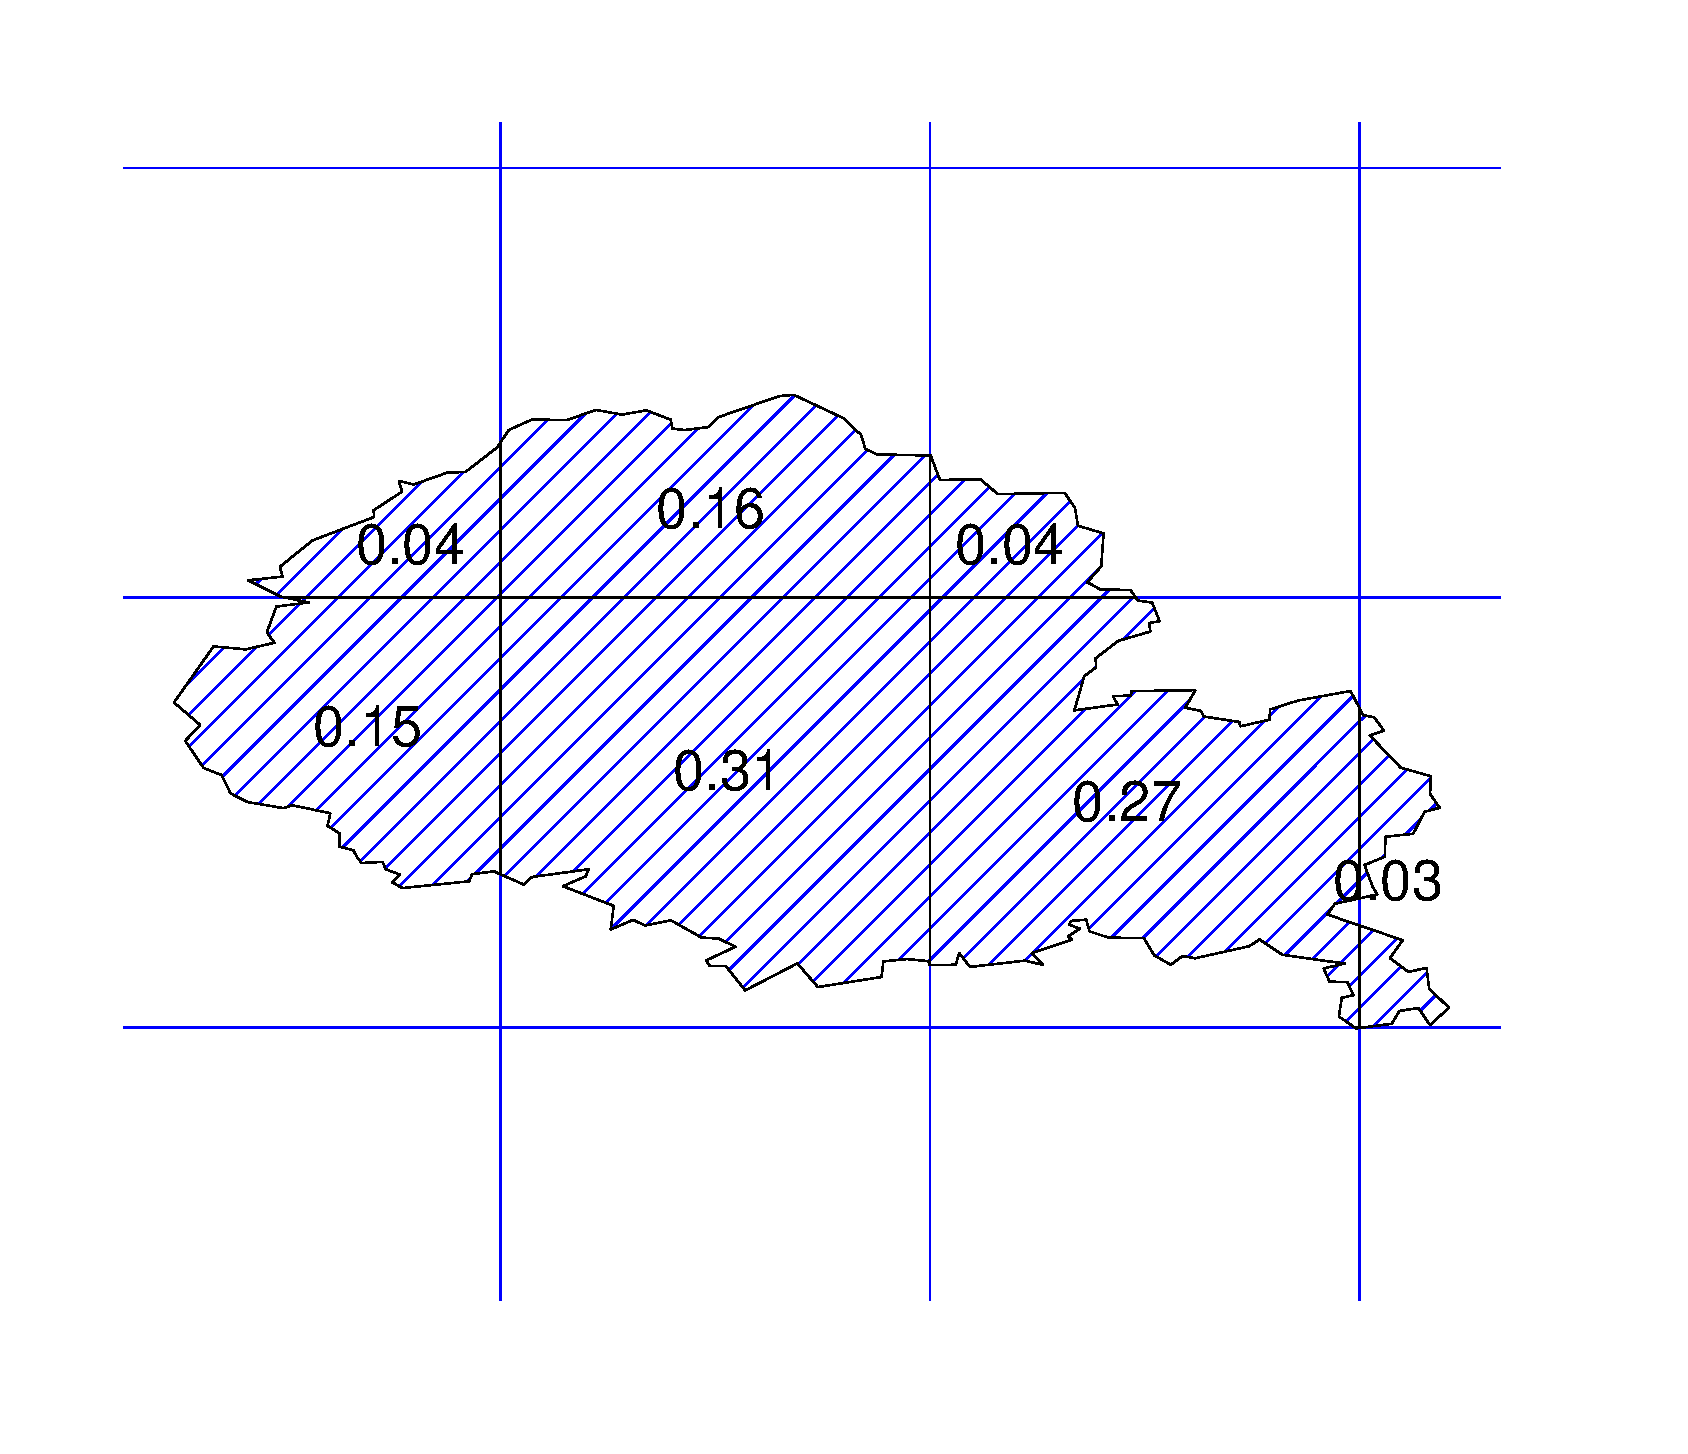
\includegraphics[scale=.18]{Zoom_grid.pdf}
\end{tabular}
\end{center}
\end{itemize}

\end{frame}
%%%%%%%%%%%%%%%%%%%%%%%%%%%%%%%%%


%\begin{frame}\frametitle{How to get $x(\bm s_{ij}^\star)$}
%
%\begin{itemize}
%\item<1-> The exposure spatial prediction  \textcolor{blue!80}{$x(\bm s_{ij}^\star)$}:
%\begin{itemize}
%\vfill\item<1-> can be available from air pollution (deterministic) \textcolor{blue!80}{dispersion models}\\
%
%\vfill\item<2-> can be computed by \textcolor{blue!80}{interpolation} of the data from monitoring stations (e.g. kriging)\\
%\vfill\item<3-> can be predicted through a Bayesian \textcolor{blue!80}{Exposure model} involving a measurement error and a spatial continuous process for the data from monitoring stations
%\end{itemize}
%\end{itemize}
%\end{frame}
%%%%%%%%%%%%%%%%%%%%%%%%%%%%%%%%%%%%%%%%%%%%%%%%%%%%%%%%%%%%%%%%%%%%
%\begin{frame}
%\frametitle{NO2  spatio-temporal model}
%\justifying
%
%$\xi_{it}$ is a zero-mean GF with the following spatio-temporal covariance function
%%
%\[
%\text{Cov}\left(\xi_{it},\xi_{ju}\right) =\left\{
%\begin{array}[c]{ccc}%
%0 &  &  \text{if} \qquad t\neq u\\
% \mathcal C(\bm s_{i},\bm s_{j}) && \text{if} \qquad t=u
%\end{array}
%\right.
%\]
%
%where $\mathcal C(\bm s_{i},\bm s_{j})$ is the Mat\'ern covariance function.
%\vspace{.5cm}
%
%%For each time point $\bm\xi_t \sim \text{Normal}(\mathbf 0, \bm \Sigma)$ and through the SPDE approach
%%\[
%%{\bm \xi}_t \Longrightarrow   \bm{\tilde \xi}_t \sim \text{Normal}(\mathbf{0},\bm Q^{-1})
%%\]
%%
%%where the precision matrix $\bm  Q$ comes from the SPDE representation.
%\end{frame}

%%%%%%%%%%%%%%%%%%%%%%%%%%%%%%%%%%%%%%%%%%%%%%%%%%%%%%%%%%
\begin{frame}
\frametitle{Spatial prediction:  $x(\bm s_{l}^\star,t) \leadsto x_{it}$}

%\begin{center}
%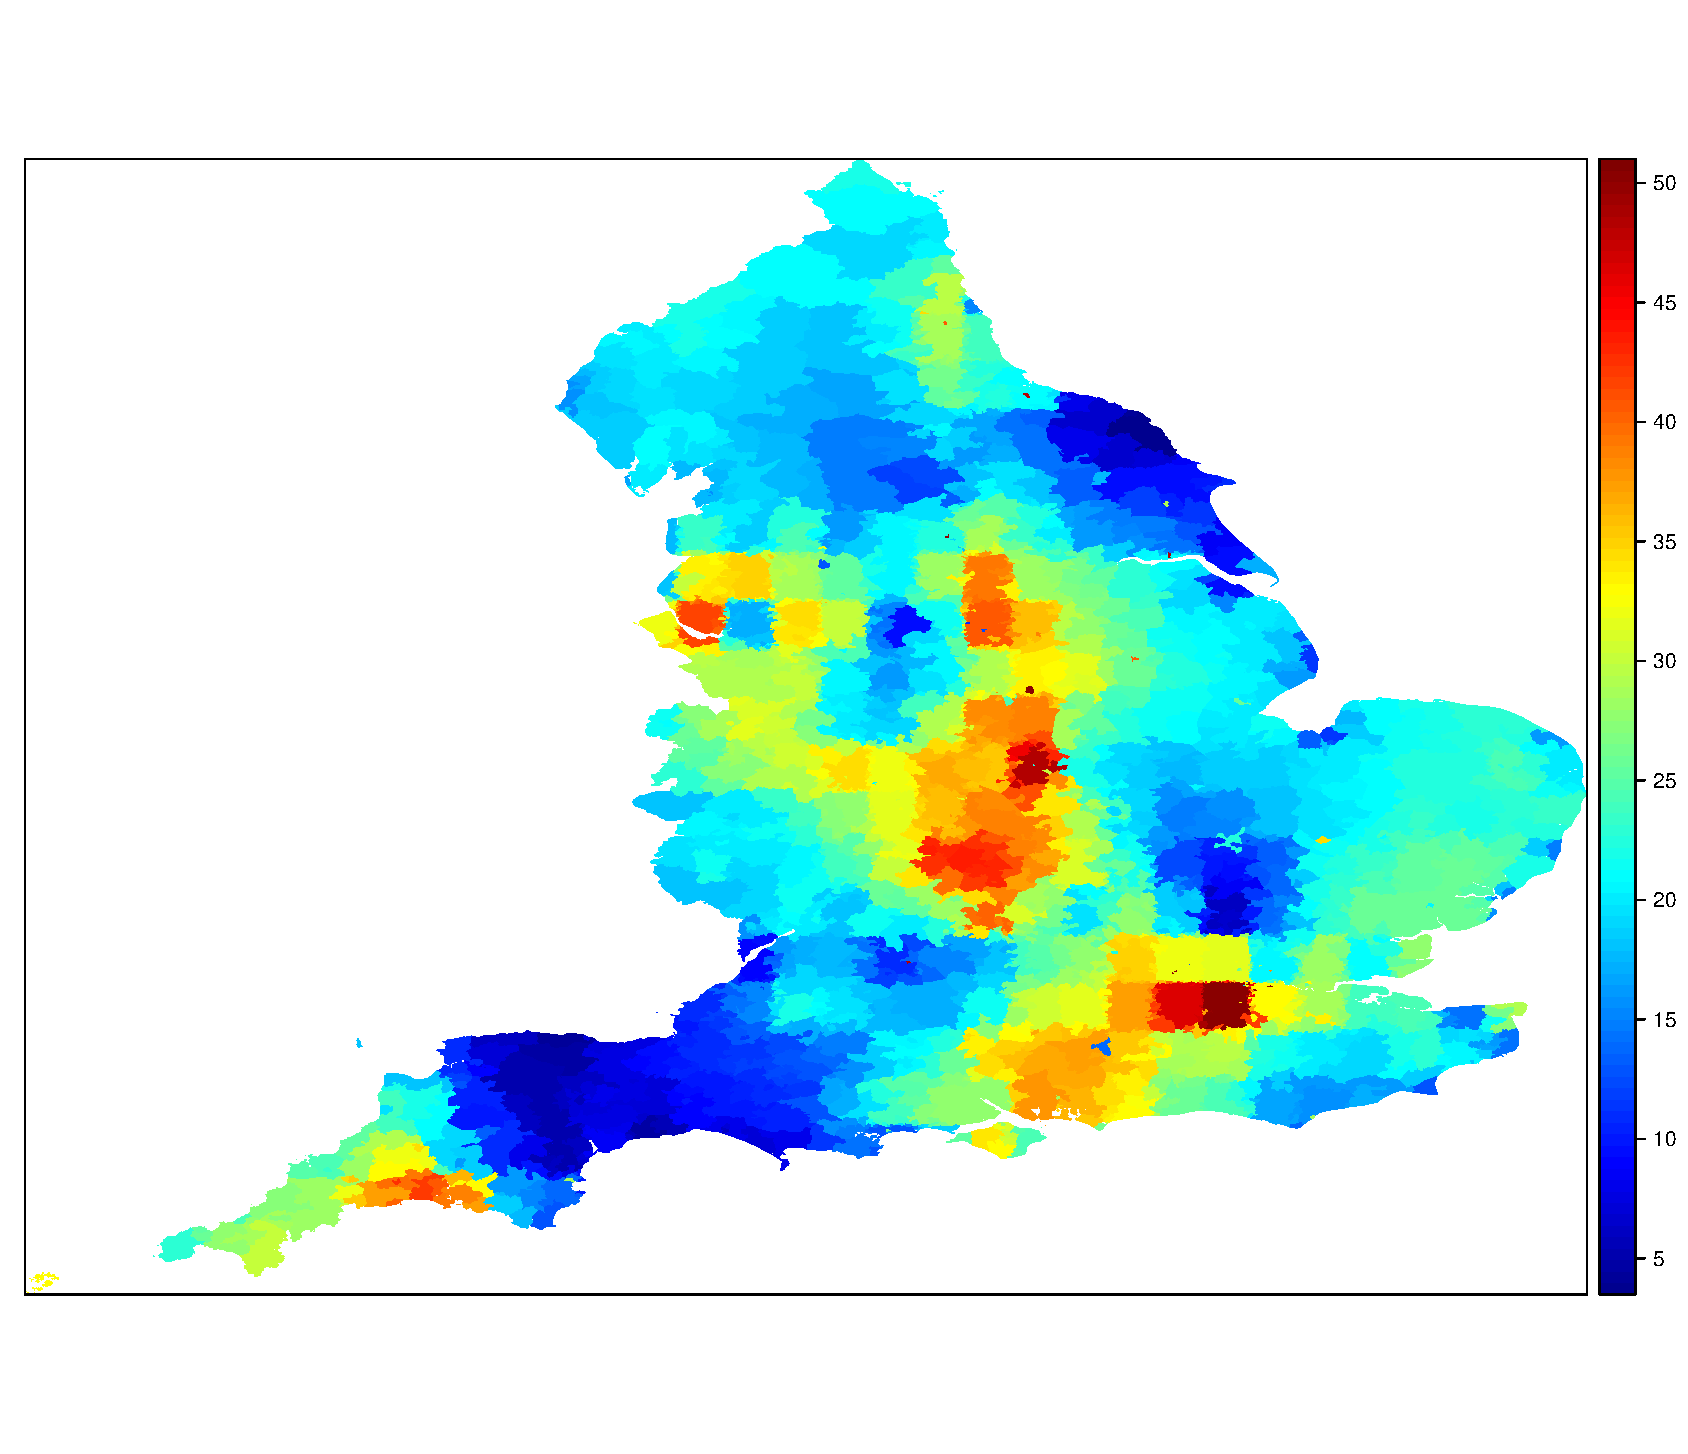
\includegraphics[scale=.2]{MSOA_NO2.pdf}
%\end{center}
\begin{center}
\begin{tikzpicture}[remember picture, overlay]
  \node (img1) at (-2.8,-3.2) {{\visible<1->{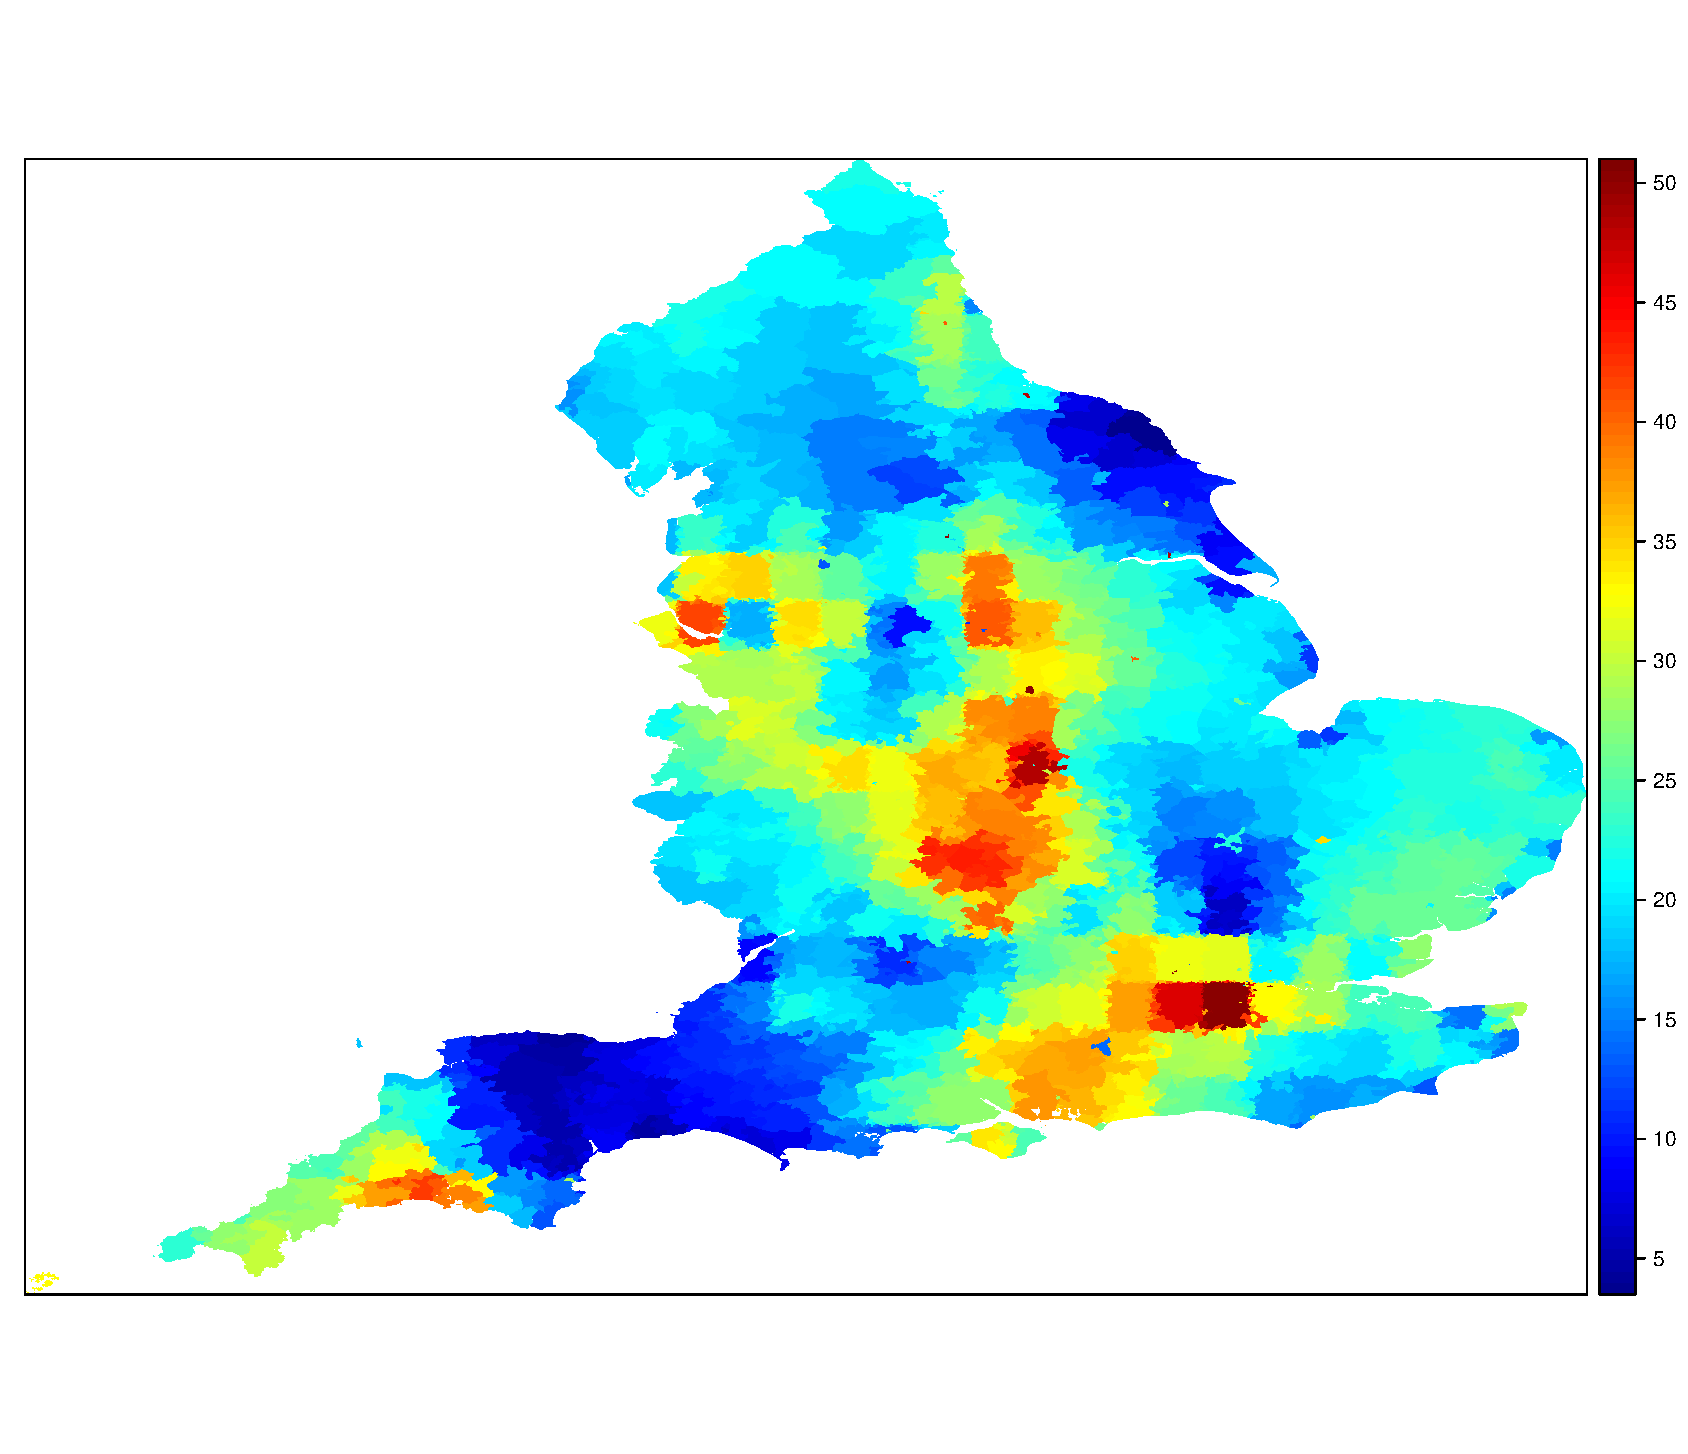
\includegraphics[scale=.2]{MSOA_NO2.pdf}}}};
 \pause \node (img2) at (3,-1.7) {{\visible<2-2>{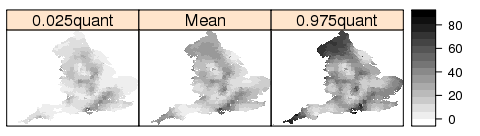
\includegraphics[scale=.5]{Posterior_ALL_NO2_MSOA_month36}}}};
  \node[below=0.5cm of img2,text width=5cm](text){{This estimates can be used for risk assessment in epidemiological studies.\\ \alert{What about uncertainty?}}};
\end{tikzpicture}
\end{center}
\end{frame}
%%%%%%%%%%%%%%%%%%%%%%%%%%%%%%%%%%%%%%%%%%%%%%%%%%%%%%%%%%%%%%%%%%%
\begin{frame}
\frametitle{Recap}
\begin{itemize}
\vfill\item Variogram to describe the data and learn about the parameters of the variance-covariance function.
\vfill\item Bayesian hierarchical modelling to provide estimates of the spatial field and associated uncertainty.
\vfill\item Useful for prediction at unobserved locations.
\vfill\item Can deal with change of support. 
\end{itemize}
\end{frame}

%%%%%%%%%%%%%%%%%%%%%%%%%%%%%%%%%%%%%%%%%%%%%%%%%%%%%%%%%%%%%%%%%%%
\begin{frame}\frametitle{Software}
\begin{enumerate}
\vfill\item MCMC
\begin{itemize}
\item Lots of R specific packages: ex.\\ 
\texttt{CARbayes}, spatial analysis with conditional autoregressive prior\\
\texttt{geoR}, geostatistical data analysis\\ 
\texttt{spTimer}, hierarchical models for spatio-temporal processes\\
\item Stand-alone general software: ex. \texttt{BUGS} (Gibbs Sampling), \texttt{Stan} (Hamiltonian Monte Carlo)
\item R packages of interface with the stand-alone software: ex. \texttt{R2OpenBUGS}, \texttt{RStan}
\end{itemize}
\vfill\item Appromixate methods
\begin{itemize}
\item \texttt{R-INLA}, Laplace Approximation for Gaussian Markov Random Fields.
\end{itemize}
\end{enumerate} 
\end{frame}
%%%%%%%%%%%%%%%%%%%%%%%%%%%%%%%%%%%%%%%%%%%%%%%%%%%%%%%%%%%%%%%%%%
\section{Some Challenges}

\begin{frame}\frametitle{Challenge: dissemination - methods}

\begin{itemize}
\item Key aspect: to propose a method that can be used by other researchers (not necessarily statisticians).
\item Reproducibility is important.
\item R packages are great - sometimes difficult for public health/social scientists.
\item R-shiny webapp can be useful.
\end{itemize}

\begin{center}
\begin{tikzpicture}[overlay]
  \node (img1) at (0,-2) {{\visible<1->{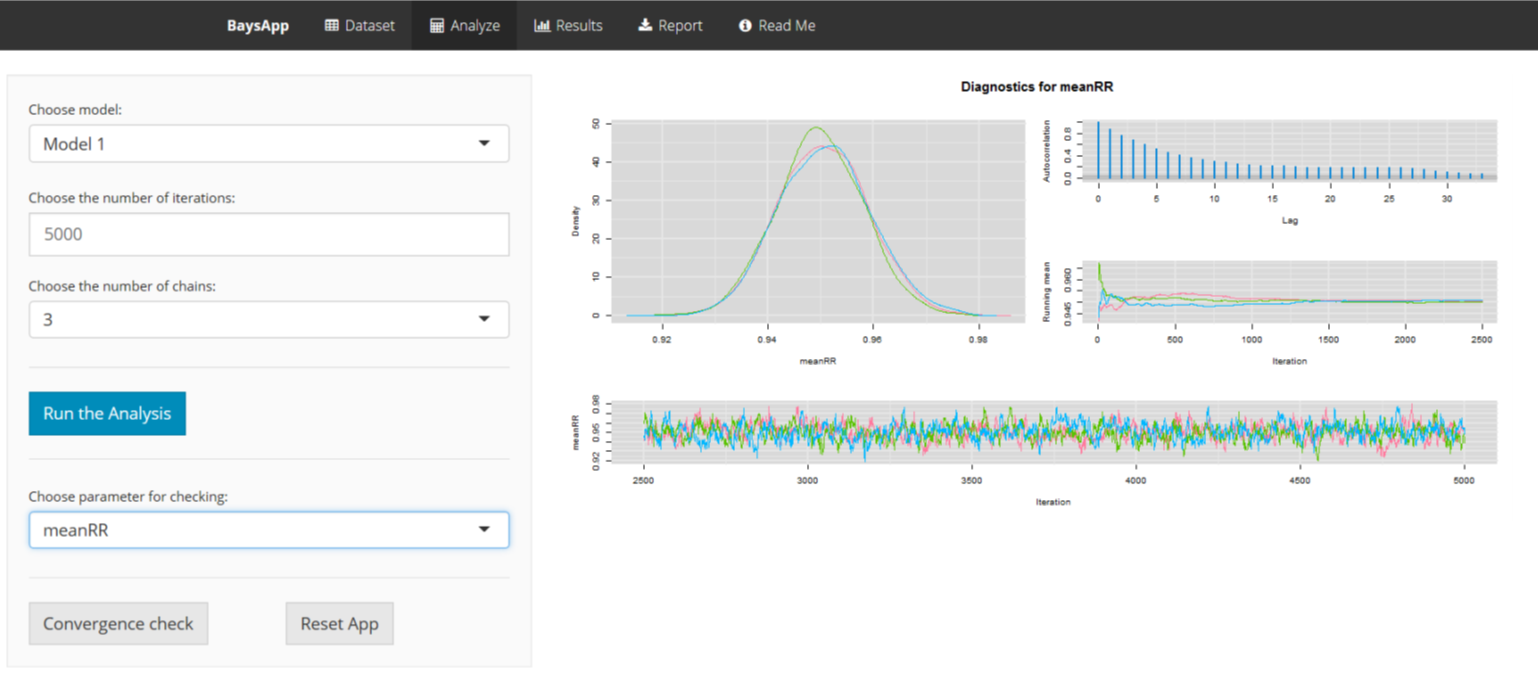
\includegraphics[height=5cm]{WebApp1}}}};
  \pause
  \node (img2) at (1,-2.2) {{\visible<2-2>{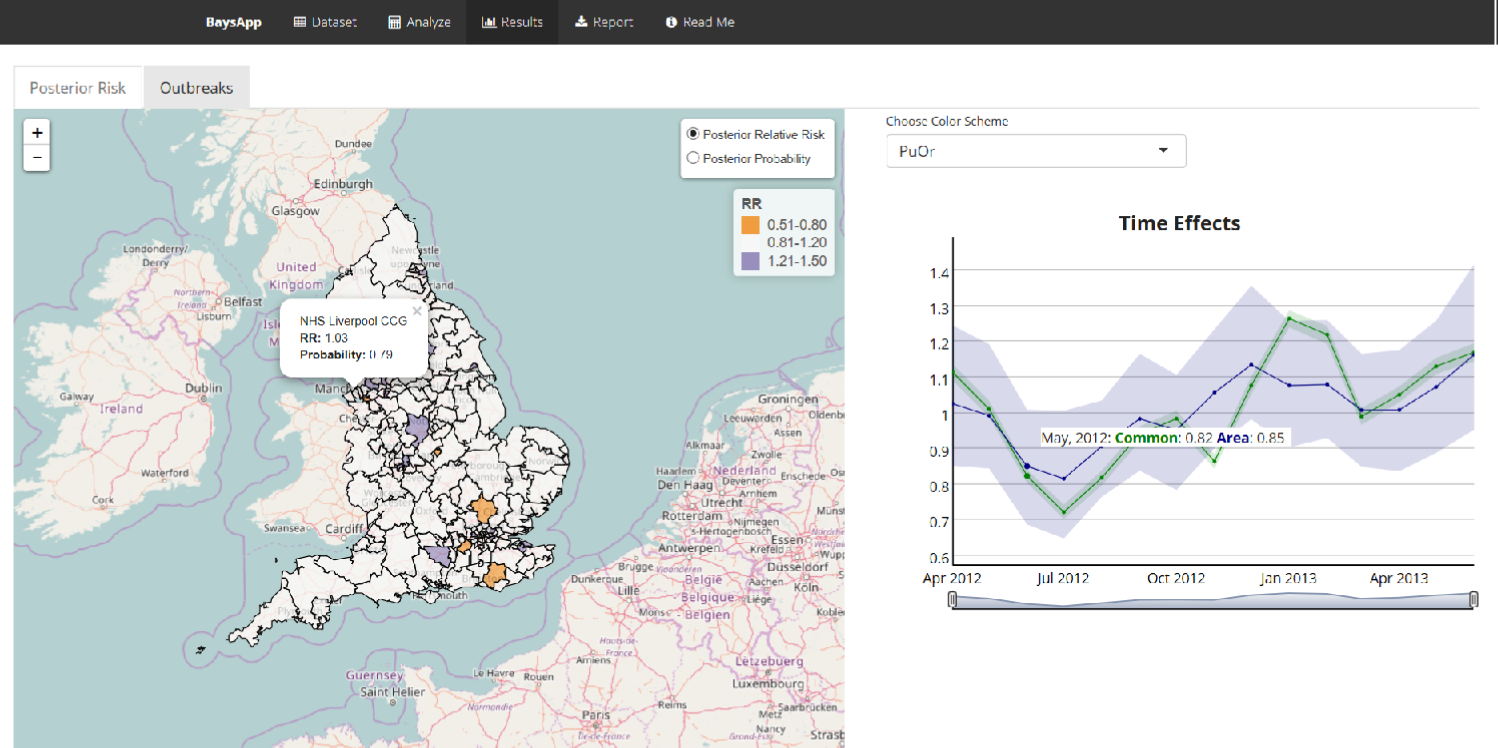
\includegraphics[height=5cm]{Webapp2}}}};
\end{tikzpicture}
\end{center}

%\begin{tabular}{cc}
%\includegraphics[scale=0.5]{Webapp1} & 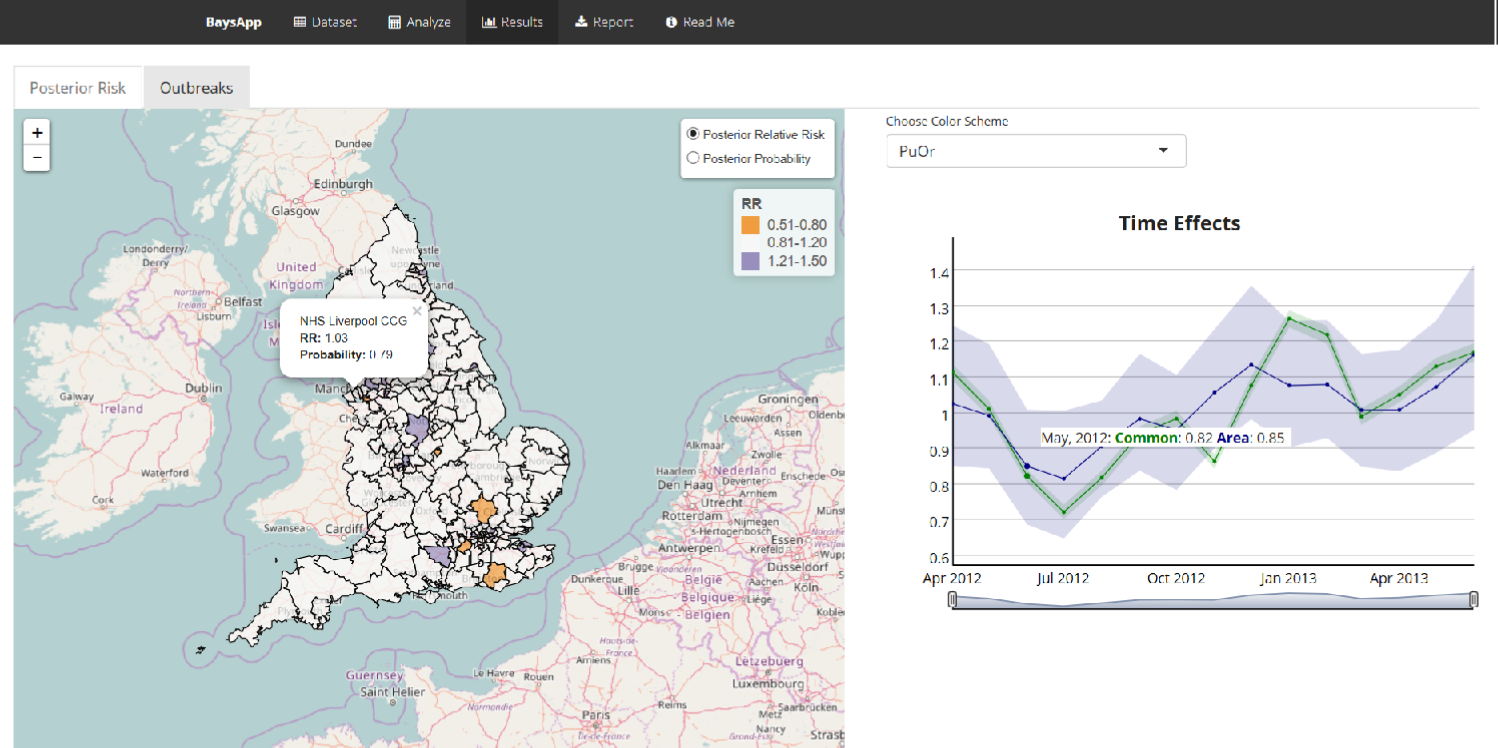
\includegraphics[scale=0.5]{Webapp2}
%\end{tabular}
\end{frame}
%%%%%%%%%%%%%%%%%%%%%%%%%%%%%%%%%%%%%%%%%%%%%%%%%
\begin{frame}\frametitle{Challenge: dissemination - maps}
\begin{itemize}
\item Cartography - scale and colors can give a different message
\end{itemize}
\begin{center}
\begin{tikzpicture}[remember picture, overlay]
  \node (img1) at (0,-3) {{\visible<1->{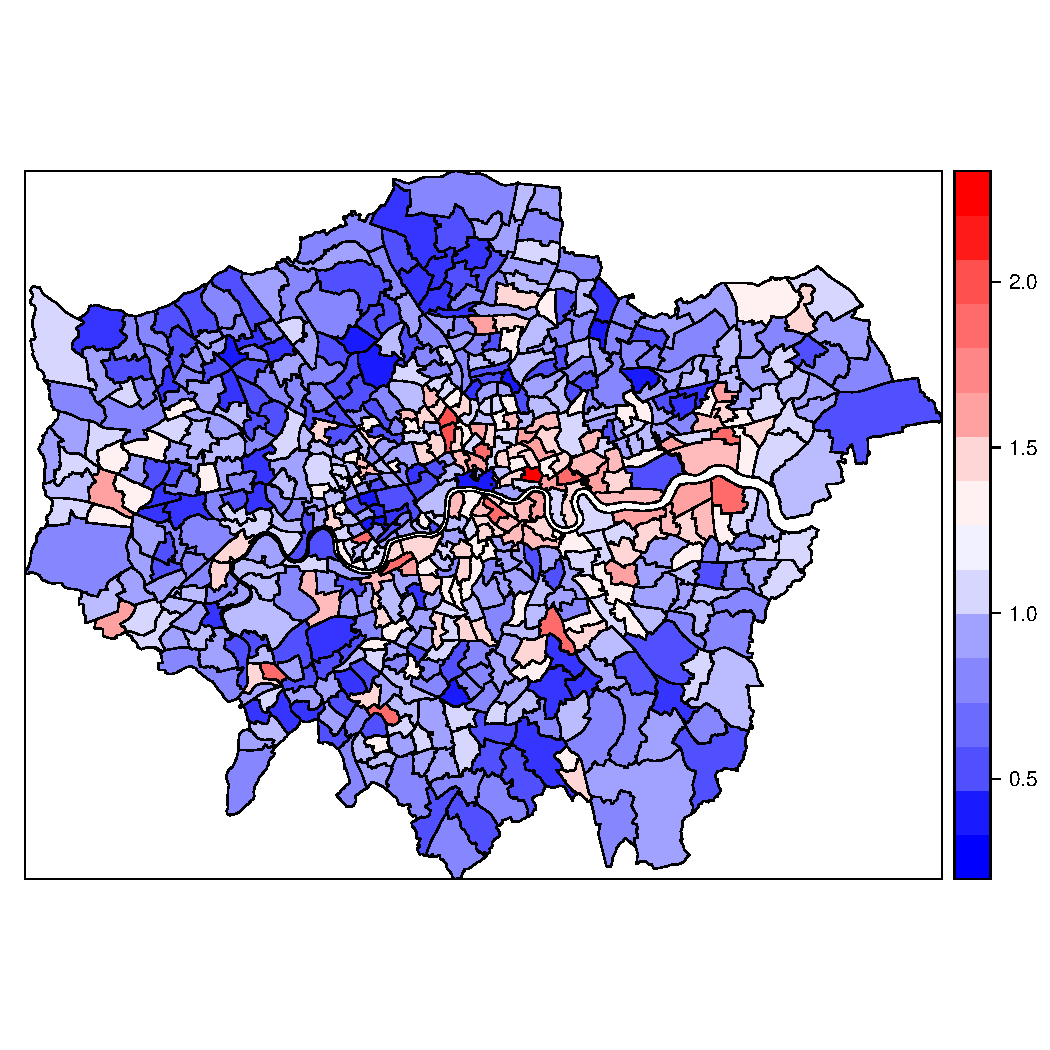
\includegraphics[height=5cm]{ClassesContinuous}}}};
%  \pause
  \node (img2) at (2,-5) {{\visible<2->{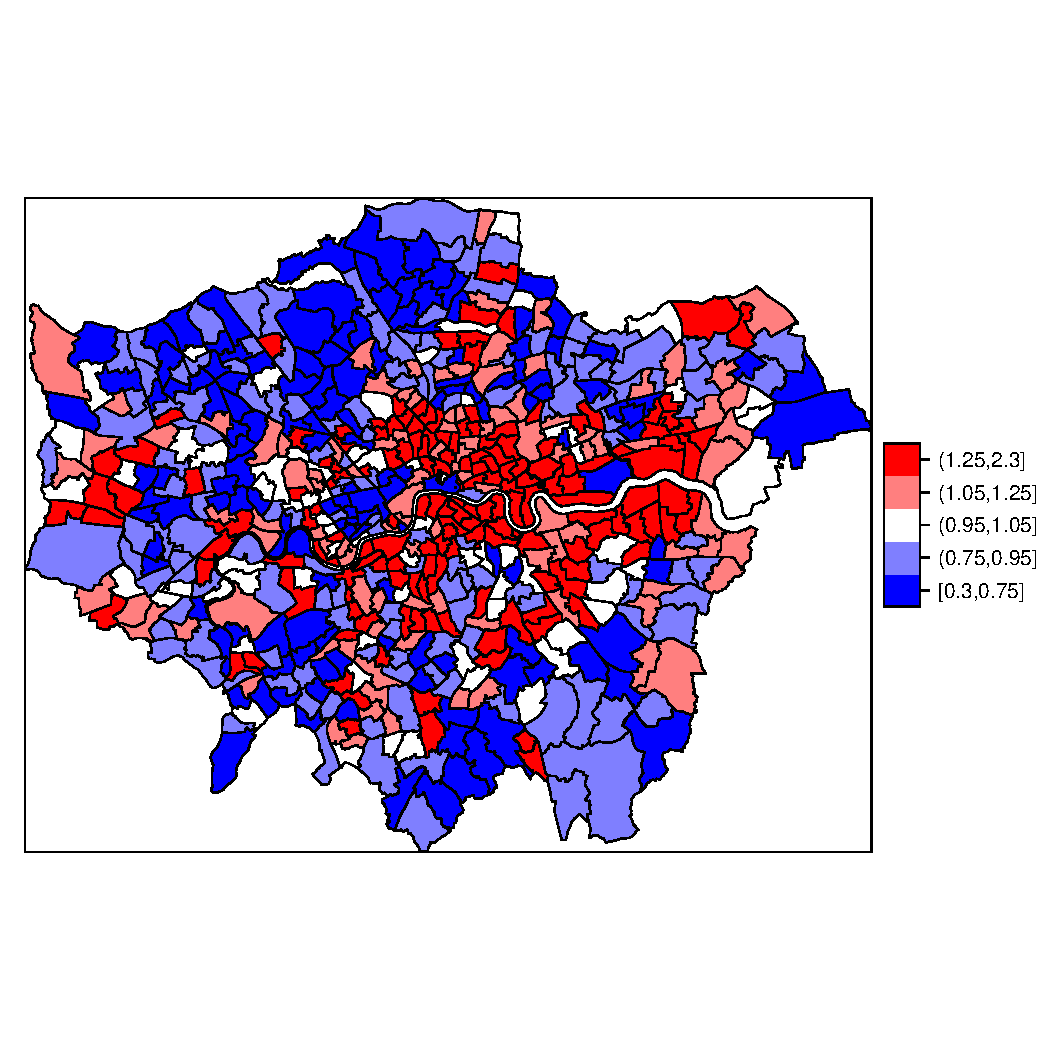
\includegraphics[height=5cm]{ClassesQuantilesDiffpoints}}}};
%  \pause
  \node (img2) at (-2,-1) {{\visible<3-3>{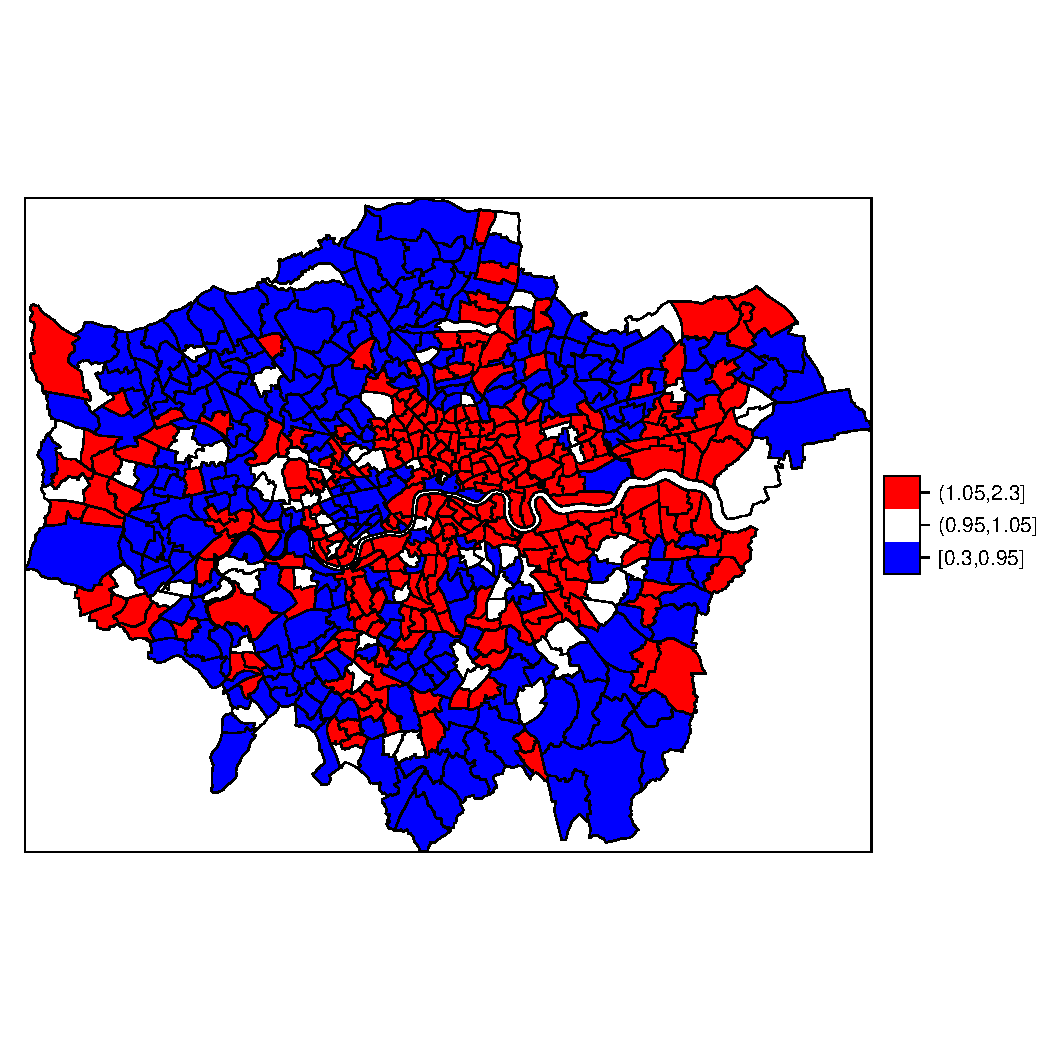
\includegraphics[height=5cm]{ClassesQuantilesLesspoints}}}};
\end{tikzpicture}
\end{center}

\end{frame}
%%%%%%%%%%%%%%%%%%%%%%%%%%%%%%%%%%%%%%%%%%%%%%%%%
\begin{frame}\frametitle{Challenge: dissemination - uncertainty}
\begin{itemize}
\item How to disseminate uncertainty\\
\begin{center}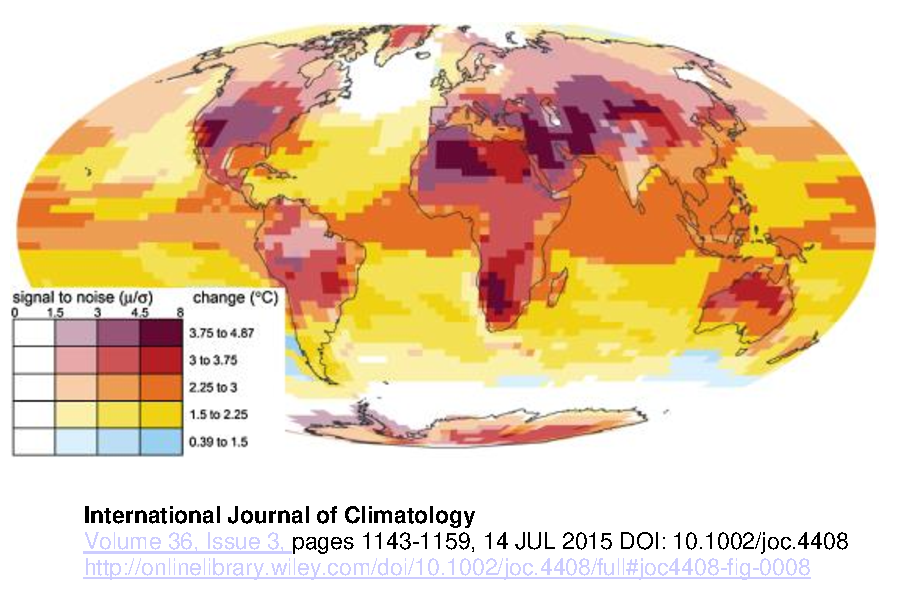
\includegraphics[scale=0.5]{Uncertainty}\end{center}

\item Who is the audience (stakeholders, general public, academic)?
\item Focus groups can help clarify the message / to find the best way to reach the audience.
$\Rightarrow$\alert{Environmental \& Health atlas} \href{http://www.envhealthatlas.co.uk/homepage/gotoatlas.html}{\beamergotobutton{EHA}}
\end{itemize} 
\end{frame}
%%%%%%%%%%%%%%%%%%%%%%%%%%%%%%%%%%%%%%%%%%%%%%%%%%
%\begin{frame}\frametitle{ challenges}
%\begin{itemize}
%\vfill\item Missing data\\ 
%$\Rightarrow$HES Opt out - what is the impact for surveillance?\\
%\vfill\item Uncertainty propagation
%$\Rightarrow$Two stage vs a joint model of exposure and health?
%\vfill\item Modelling several conditions or correlated exposures\\
%$\Rightarrow$ Non parametric methods 
%...
%\end{itemize}
%\end{frame}
%%%%%%%%%%%%%%%%%%%%%%%%%%%%%%%%%%%%%%%%%%%%%%%%%

\begin{frame}
\frametitle{Acknowledgements}
\begin{itemize}
\vspace{10pt}\item Areti Boulieri (IC)
\vspace{10pt}\item James Bennett (IC)
\vspace{10pt}\item Nicky Best(GSK)
\vspace{10pt}\item Michela Cameletti (UNIBG)
\vspace{10pt}\item Virgilio Gomez-Rubio (Castillia-LaMancha)
\vspace{10pt}\item Anna Hansell (IC)
\vspace{10pt}\item Monica Pirani (IC)
\vspace{10pt}\item Sylvia Richardson (MRC-BSU)
\end{itemize}
\end{frame}
%%%%%%%%%%%%%%%%%%%%%%%%%%%%%%%%%%%%%%%%%%%%%%%%%

\begin{frame}
\frametitle{References}
\begin{enumerate}
\item \fontsize{8}{8}\selectfont{Small area}
\begin{itemize}
\item \fontsize{8}{8}\selectfont{Best, N., Richardson, S., and Thomson, A. (2005). A comparison of Bayesian spatial models for disease mapping. Statistical Methods in Medical Research, 1(14), 35-59.}
\item \fontsize{8}{8}\selectfont{Lee, D. (2011).A comparison of conditional autoregressive models used in Bayesian disease mapping. Spatial and Spatio-Temporal Epidemiology, 2(2), 79-89}
\item \fontsize{8}{8}\selectfont{Lawson A., Banjeree, S., Ugarte, L., Haining, R. (2016) Handbook of spatial epidemiology. CRC.} 
\item \fontsize{8}{8}\selectfont{Jackson C, Best N. and Richardson S. (2008) Hierarchical related regression for combining aggregate and individual data in studies of socio-economic disease risk
factors. J Royal Statistical Society Series A: Statistics in Society 171(1):159-178}
\end{itemize} 
\item \fontsize{8}{8}\selectfont{Geostatistics}
\begin{itemize}
\item \fontsize{8}{8}\selectfont{Banerjee, S., Carlin, B., and Gelfand, A. (2004). Hierarchical Modeling and Analysis for Spatial Data. Monographs on Statistics and Applied Probability. Chapman \& Hall.}
\item \fontsize{8}{8}\selectfont{Diggle, P. and Ribeiro, J. (2007). Model-Based Geostatistics. Springer.}
\item \fontsize{8}{8}\selectfont{Gelfand, A., Diggle, P., Fuentes, M., and Guttorp, P., editors (2010). Handbook of Spatial Statistics. Chapman \& Hall.}
\item \fontsize{8}{8}\selectfont{Wikle, C. (2003). Hierarchical models in environmental science. International Statistical Review, 71(2), 181-199.}
\end{itemize}
\end{enumerate}

%\tiny {\bibliography{refs}}
%\bibliographystyle{asa}
\end{frame}

\end{document}